%\documentclass[12pt]{report}   % SUBMISSION TO GRAD SCHOOL
\documentclass[12pt,twoside]{report}  % TWOSIDE DUPLEX OUTPUT
\usepackage{setspace}
\usepackage{buthesis}
\usepackage{amsmath,amssymb,graphicx,amsfonts,amsthm}
\usepackage{verbatim}
\usepackage{epsfig}
\usepackage{wrapfig}
\usepackage{latexsym,amsfonts,amscd}
\usepackage{changebar}
\usepackage{enumerate}
\usepackage{yfonts}

\usepackage{mathtools,bbm,enumerate}
\usepackage{mathrsfs}
%\usepackage{caption}
%\usepackage{subcaption}

% Do you use TikZ?
\usepackage{tikz}
%\usepackage{pgfmath}
\usetikzlibrary{decorations}
\usetikzlibrary{shadows}

% Used only for example text
%\usepackage{lipsum}
\DeclareMathOperator{\diag}{diag}

\usepackage[footnotesize,bf]{caption}  % Reduces caption font sizes

\graphicspath{ {./images/} }

%%%%%%%%%%%%%%%%% Fancy chapter headings %%%%%%%%%%%%%%%%%%%
\usepackage[Bjarne]{ThesisFncychap}
% Redefine alphano commands

%%%%%%%%%%%%%%%%%%%%%%%%%%%%%%%%%%%%%%%%%%%%%%%%%%%
\makeatletter
  
  \ChNameVar{\Huge\sc}    % sets the style for name
  \ChNumVar{\Huge\sc}         % sets the style for digit
  \ChTitleVar{\Huge\bf\centering} % sets the style for title
  \ChRuleWidth{4pt}        % Set RW=4pt
  %\ChNameUpperCase         % Make name uppercase
  \ChNameAsIs         % Make name uppercase
  \ChTitleAsIs

  \renewcommand{\DOCH}{%
    %\setlength{\fboxrule}{\RW} % Let fbox lines be controlled by
                               % \ChRuleWidth
    %\fbox{\CNV\FmN{\@chapapp}\space \CNoV\thechapter}\par\nobreak
    \thispagestyle{empty}
    \vskip 80\p@
    \begin{center}
    %\CNV\FmN{\@chapapp}\space \CNoV\thechapter\par\nobreak
    \CNV\FmN{\@chapapp} \TheAlphaChapter\par\nobreak
    \begin{tabular*}{\textwidth}{c}
      \hline
    \end{tabular*}
    %\line(1,0){5in}\\
    \end{center}
    %\vskip 20\p@
    }

  \renewcommand{\DOTI}[1]{%
    \CTV\FmTi{#1}\par\nobreak
    \vskip 40\p@
    {\newpage}
    }
  \renewcommand{\DOTIS}[1]{%
    \CTV\FmTi{#1}\par\nobreak
    \vskip 40\p@
    }
\makeatother


%%%%%%%%%%%%%%%%%%%%%%%%%%%%%%%%%%%%%%%%%%%%%%%%%%%%%%%%%%%%

%-----------------------------------------------------------------
%% Control the fonts and formatting used in the table of contents, list of
%% figures, and list of tables
\usepackage[titles]{tocloft}


%% Aesthetic spacing redefines that look nicer to me than the defaults.
\setlength{\cftbeforechapskip}{-1ex}
\setlength{\cftbeforesecskip}{-3.5ex}
\setlength{\cftbeforesubsecskip}{-3.5ex}
\setlength{\cftbeforetabskip}{-3.5ex}
\setlength{\cftbeforefigskip}{-3.5ex}
%-----------------------------------------------------------------

\dissertation % This *is* what you're writing, right?

% Information about the document
%-----------------------------------------------------------------
\title{
The Building Game and Other Discrete Geometric Models for the Self-assmbly of Polyhedral Molecular Structures 
}
\author{Daniel C. L. Johnson}
\degree{Doctor of Philosophy}
\department{The Division of Applied Mathematics}
\previousdegrees{
		B.S., Rensselaer Polytechnic Institute; Troy, NY, 2009\\ 
		Sc.M., Brown University; Providence, RI, 2012}	
\thesismonth{May} \thesisyear{2015}
%-----------------------------------------------------------------

\begin{document}

\doublespacing
\begin{preliminaries}
\maketitle

\copyrightpage

\begin{signature}
  \director{Govind Menon, Ph.D., Advisor}
  \reader{Committee Member II, Ph.D., Reader}
  \reader{Committee Member III, Ph.D., Reader}
\end{signature}

\begin{vita}
  %\lipsum[1-2]

\end{vita}

\begin{acknowledgments}
  %\lipsum[3-4]

\end{acknowledgments}

\begin{abstract}
  %\lipsum[6-8]

  \thispagestyle{empty}
  % Do you want this page to exist in the numbering?
%  \thispagestyle{empty}
%  \if@twoside
%    \addtocounter{page}{-2}  
%  \else
%    \addtocounter{page}{-1}
%  \fi
\end{abstract}

% Why double-space toc,lof, and lot?
\begin{spacing}{1}
  \tableofcontents
  \clearpage{\pagestyle{empty}\cleardoublepage}

  \footnotesize
  \fontsize{11.5pt}{12.5pt}\selectfont
  \listoftables
  \clearpage{\pagestyle{empty}\cleardoublepage}

  \listoffigures
  \clearpage{\pagestyle{empty}\cleardoublepage}
  \normalsize
\end{spacing}

\end{preliminaries}

\pagestyle{myheadings}

%------------------------ CONTENT ------------------------%
%-----------------------------------------------------------------
%% Shortcuts
\newtheorem{mythm}{Theorem}
\newtheorem{mylem}{Lemma}
\newtheorem{mycor}{Corollary}
\newtheorem{mydef}{Definition}

\newcommand{\colorA}{white}
\newcommand{\colorB}{black}
\newcommand{\colorAsm}{w}
\newcommand{\colorBsm}{b}
\newcommand{\poly}{$\mathscr{P}$}
\newcommand{\Poly}{\mathscr{P}}
\newcommand{\PolyGraph}{\textswab{G}_\mathscr{P}}
\newcommand{\faceset}{F\left(\mathscr{P}\right)}
\newcommand{\spc}{ }
\newcommand{\xj}{$x^j$}
\newcommand{\xk}{$x^k$}
\newcommand{\Sjk}{$S_{jk}$}
\newcommand{\Skj}{$S_{kj}$}
%\newcommand{\G}{{G_\mathscr{P}}}
\newcommand{\G}{{G}}

\chapter{Introduction}
%\lipsum[21-40]

%\nocite{Lax1956,Cooley1965,Banach1924}
\section{Introduction}

Self-assembly is a class of formation process in which a product is constructed with out explicit manipulation of its parts. Many---often identical---parts come together by utilizing the dynamics of their environment to create a finished structure. Sometimes such assemblies can be encouraged can be encouraged by manipulating broadly controlled parameters of the assembly environment such as temperature and solution content. 

There are many examples of both natural and synthetic self-assembly process that take a wide variety of length scales and serve a plethora of functions. An area of much active research is the self-assembly of RNA, proteins, and viral capsids. These biological processes act on the nano scale and, while it is known that their formation can be aided by a variety of secondary mechanisms such as helper RNA, the formation process is not well understood in general. Synthetic examples of molecular self assembly include the formation of supramolecular cages. These supramolecular structures that can encapsulate a smaller molecule show promise in contributing to a number of medical and scientific fields including drug delivery and nano-scale circuits. 

In general, the processes of biological self-assembly are not well understood due to difficulties arising from their small length scale. Conversely, synthetic self-assembly processes often lack the complexity and sophistication of their biological equivalents. The goal of our research is to explore discrete geometric models of self assembly. By using analysis made possible by the simplicity of said models, important properties of the processes are to be identified. Of primary importance is identifying the pathways of formation which consist of a specific order in which unfinished intermediate states are visited before the assembly is completed. It is thought that these pathways are often robust in the sense that the process follows a very small, and sometimes unique, number of pathways to form the end product. Also of interest is identifying mechanisms by which failed or flawed formations can be avoided or minimized. Possible strategies include the selection of specific precursors, the selection of solution, and the mid-assembly control of experimental parameters. 

\subsection{Self-Folding Polyhedra}

In experiment, Pandey et al have been able to form closed polyhedral structures from the self-folding of flat polyhedral nets. Using photolithography, these nets are cut from a two dimensional sheet with great precision. By adding a specific amount of solder at the net's hinges, surface tension from the melted solder causes the net to fold up into the closed polyhedron. Several different polyhedra have been attempted with varying degrees of success. It has been argued that the geometric structure of the polyhedron are largely determinant of the net's propensity to successfully assemble into the polyhedron. In some cases, two distinct polyhedral isomers can be formed from the same net.

\subsection{Molecular Cages}

Self-assembly of molecular cages are the subject of much active research. By isolating molecules of interest inside a molecular cage, targeted application of these molecules is theoretically possible. This has enormous implications in the medical industry. Additionally, by creating a grid-like network of such cages, it may be possible to construct functional electric circuitry at the nano scale. 

Fujita et. al. have theorized and subsequently synthesized a family of organometallic cages consisting of metallic connector molecules (M) that each connect four bent ligand molecules (L). With the M molecules as vertices and the L molecules as edges, they can form polyhedral cages. Due to geometric constraints, the number of M and L molecules in  a completed cage must satisfy  $|M| = k$ and $|L| = 2k$ for $k \in 6, 12, 24, 30, 60$. Each of these five choice of $k$ results in a cage that geometrically resembles a specific Archemedian solid. 

In one experiment, two different ligands ($L_1$ and $L_2$) with slightly different bend angles were used. As the ratio of $L_1:L_2$ was varied, each ratio only resulted in the formation of one of the possible cages. More specifically, for ratios $L_1:L_2 < 0.25$ only $M_{12}L_{24}$ formed and for  $L_1:L_2 > 0.25$ only $M_{24}L_{48}$ was formed. This steep and curious cutoff thus far defied tangible explanation. With the help of our discrete models, we hope to shed light on this phenomena. 

In experiments by Liu et al, polyhedral supramolecular cages made from different molecular species were synthesized. Theoretically, tiling type behavior of the molecular species is possible, but it was not observed. Additional experiments in which copies of two types of molecular species could be combined to form two different polyhedral cages were proposed. It is unknown if both potential polyhedral cages would form or if one would be significantly more favorable over the other. Being able to predict the results of such experiments via mathematical analysis and simulation would be a significant contribution toward optimizing strategies for the self-assembly of supramolecular cages. 

\subsection{Viral Capsid Assembly}

With forces such as friction playing a much bigger role on their length scale, biological viruses are remarkable at robustly replicating themselves. While this topic has been well studied and a wide variety of mechanisms have been evidenced to contribute, there still is no general understanding of the process in which a virus' capsid is formed. Viral capsids come in many shapes and sizes, but a significant portion of them are icosahedral in structure. Understanding of their pathways of formation may be a key to preventing or slowing down replication.  

\subsection{RNA and Protein Folding}

Protein and RNA folding are active fields of research. If we can predict the structure of a RNA or protein based on its amino acid sequence, we will know more about its biological function. As many human and animal disorders are caused by proteins folding abnormally, their cures may lie in the understanding of the folding pathway. While we do not directly consider applications relating to RNA and protein folding, success with the above problems may also provide insights for this complex topic. 

Just as in self-assembly, folding constitutes the passage between several intermediate states along a pathway leading to formation of a final structure. In both examples, formation pathways are thought to be nearly unique. The identification of these pathways may allow for the targeted intervention at a specific intermediate in the case of abnormal folding behavior. 

\section{Models of Self-Assembly}
\subsection{The Building Game}

First proposed by Zlotnick et al, the Building Game (BG) is a discrete attachment model that simulates the sequential construction of polyhedral structures. The BG can describe the behavior of many two dimensional face molecules interacting in a solution and bonding together to ultimately form polyhedral molecule.

 The building game (BG) for a polyhedron $\mathcal{P}$ begins with a single face of $\mathcal{P}$ and iteratively attaches faces to the existing partially formed polyhedron until all faces of $\mathcal{P}$ are present. We denote the set of $\mathcal{P}$'s faces, edges, and vertices as $F(\mathcal{P}),E(\mathcal{P}),$ and $V(\mathcal{P})$ respectively. A building game \textbf{pathway} is a linear ordering $f_1,f_2,f_3,\ldots,f_N$ of the faces of $\mathcal{P}$ such that for $j = 2,\ldots,N$ there exists edges $e_1,e_2,\ldots,e_k \in E(\mathcal{P})$ with  $k \geq 1$ satisfying
$$\left(e_1\cup\cdots\cup e_k \right)\subset \left(f_j\cap\left(\bigcup_{i=1}^{j-1}f_i\right)\right)$$
Since the order and location of attachment in the building game can vary, many partially formed polyhedra, called \textbf{intermediates}, are possible. Each intermediate $x$ can be represented as $x = \cup_{i=1}^tf_i$ where $f_1,\ldots,f_t,\ldots,f_N$ is a BG pathway. For a given polyhedron, we are interested in enumerating all of the distinct intermediates up to rotational equivalence. The  \textbf{attachment sites} of an intermediate $x$ are the set of faces $\{f_k\}$ such that $f_k\cap x = e_1\cup e_2 \cup \cdots$ for some edges $e_1,e_2,\ldots \in E(\mathcal{P})$. In other words, the attachment sites are the places in which a new face may join $x$ as part of a valid BG pathway.

\begin{figure}[!h]
%\centering
%\includegraphics[width=0.8\textwidth]{bg.png}
\caption{Dodecahedron building game example.}
\label{fig:bg}
\end{figure}

The \textbf{state space} for a particular polyhedron $\mathcal{P}$ is a graph that represents the space of all distinct intermediates and the BG pathways for $\mathcal{P}$. Each node of the state space represents a single intermediate and a connection exists between two nodes if it is possible to construct one of the corresponding intermediates by adding a single face to the other. Each path through the state space, starting at an intermediate with one face and ending at the intermediate with all faces, represents one of the polyhedron's BG pathways. 

\begin{figure}[h]
%\centering
%\includegraphics[width=0.8\textwidth]{cube_bg.png}
\caption{The state space of the cube.}
\label{fig:cube_bg}
\end{figure}


%\begin{figure}[h]
%\centering
%\includegraphics[width=0.8\textwidth]{dodecahedronSS.png}
%\caption{Configuration space of the dodecahedron}
%\label{fig:dodecahedronSS}
%\end{figure}


For a state space edge going between an intermediate with $k$ faces to one with $k+1$ faces, the \textbf{degeneracy number} is the number of different attachment sites on the $k$-faced intermediate that will produce the $k+1$-faced intermediate. For example, the state space edge between the cube intermediate with 1 face and the intermediate with 2 faces has degeneracy number 4 since each of the first square's four edges will form the same intermediate when a second square is attached. 


As we consider polyhedra with more and more faces, there is a combinatorial explosion in the number intermediates in state space. While the 6-faced cube state space has only 8 vertices and 9 edges, the 20-faced icosahedron state space has 2,649 vertices and 17,241 edges and the 26-faced truncated cuboctahedron state space has 1,525,605 vertices and 17,672,377. We have computed the BG state space for all polyhedra in the Platonic, Archimedean, and Catalan solid classes of up to 30 faces. Due to computational constraints, we do not compute the BG state space for larger polyhedra, but we are exploring the possibility of non-enumerative exploration of the state space of large polyhedra in the future. 

The Building Game suffers from the fact that it only allows one end product to form and cannot model physically realistic formation errors. However its simplicity is a feature that aids analysis. We discuss models that do capture formation errors below.  


\subsection{Folding}
Another model that we refer to as the Folding Model, was used by Pandey et al to model the folding style self-assembly of meso-scale metallic polyhedra. In this model, a polyhedron's net is sequentially folded up into the finished polyhedron. At each stage one vertex is closed to form a pyramidal structure by a folding move. In analogy with the building game, we can define folding intermediates to be partially folded states and a state spaces where intermediates are connected if one can form the other with a single fold. The state space and corresponding intermediates are shown in figure~\ref{fig:fold_octa}. 

Interestingly, each polyhedron may has multiple nets. In fact, the number of distinct nets grows rapidly with the size of the polyhedron. Certain nets have different folding pathways and measuring the favorability of one of these nets over another introduces an design problem. If nets that fold into the completed polyhedron most reliably can be identified, the efficiency of the self-assembly process can be optimized.

\begin{figure}[h]
%\centering
%\begin{subfigure}[b]{0.45\textwidth}
%NEEDS FILE
%%\includegraphics[width=\textwidth]{folding_state_space.png}
%\caption{State Space}
%\label{fig:fold_ss}
%
%\end{subfigure}
%~
%\begin{subfigure}[b]{0.4\textwidth}
%NEEDS FILE
%%\includegraphics[width=\textwidth]{folding_ints.png}
%\caption{Intermediates}
%\label{fig:folding_ints}
%
%\end{subfigure}
%
%\caption{The folding model on the octahedron.}
\label{fig:fold_octa}
\end{figure}

As a feature, this model has been shown to allow folds that do not result in the initially intended polyhedron and can terminate in other polyhedra and blocked states. In figure~\ref{fig:fold_ss}, the red connections represent folds that can still result in the octahedron while the green connections cannot. Many of the intermediates that cannot fold into the octahedron end up folding into a non-convex boat intermediate (84).

Like in the building game, the state space of the folding model experiences a combinatorial explosion as the number of faces the polyhedron has increases. Surprisingly, the building game can be used to recover the part of the folding state space which allows folding to the originally intended polyhedron. 
\begin{mythm}
Given a polyhedron $\mathcal{P}$, there exists a second polyhedron $\mathcal{P}'$ such that the sub-graph of folding state space containing intermediates that can still fold into $\mathcal{P}$ can be recovered from the building game state space for $\mathcal{P}'$.  
\end{mythm}


\subsection{Local Rules}

A large number of previously studied models for self-assembly can be classifies as \textit{local rules} based approaches. Such models typically consist of a collection of components that can be combined according to a specified grammar. While a basic idea, the variety off possible component and grammars makes this a widely flexible class of models. Schwartz et al used such a model to describe the assembly of viral capsids. Since these capsids are fundamentally composed of proteins that can each assume a number of conformations. By putting a grammar on the ways in which proteins of different conformation can combine, they we able to successfully form a variety of viral capsids in simulation. While this class of models is powerful, we have not actively pursued any such models. In the future, it may be work trying to use a local rules model that is akin to the building game, but will be sufficiently general to allow formation errors as in the folding model.    

\section{Dominant Formation Pathways}

The concept of formation pathways that occur with overwhelming frequency relative to the myriad of other theoretically possible pathways is a primary focus of our work. To identify the nature of such dominant pathways is to identify the mechanism of self-assembly itself. This knowledge would hopefully enable the formation of the self-assembled products to become more efficient and expedient, or in cases such as biological viruses, inhibit it altogether. There are several means, both quantitative and qualitative, by which we seek to identify and study these dominant pathways. 

\subsection{Markov Processes}


We first define a Markov Chain on the Building Game state space and identify the corresponding stationary distribution. 

Associated with each intermediate $x_j$, we have the the combinatorial statistic $E_j \doteq -E(x_j)$ which is negative one times the number of edges in $x_j$ at which two faces meet. Thus, $E_k-E_j$ represents the number of such edges added (or removed) when a face is added to (or removed from) $x_j$ to form $x_k$. This statistic $E_j$ is an idealization of a bond energy within an intermediate.

We define the Markov chain $X_t$ by the transition rule $P_{jk} \doteq P(X_{t+1} = x_k | X_t = x_j)$, with the heuristic that it should be more likely for an intermediate to add a face in a location in which more new edge connections can be formed.

% \begin{numcases}{P_{jk} =}
%        \frac{1}{z_j}s_{j,k}e^{-\frac{1}{2}\beta\left(E_k-E_j\right)}  & $j \neq k, j \leftrightarrow k$ \\
%        \frac{1}{z_j}\phi_j \label{eq:A} & $j = k$\\
%        0 & $j \neq k, j \not\leftrightarrow k$
%        \end{numcases}

$$
 P_{jk} = \begin{cases}
        \frac{1}{z_j}S_{j,k}e^{-\frac{1}{2}\beta\left(E_k-E_j\right)}  & j \neq k, j \leftrightarrow k \\
        \frac{1}{z_j}\phi_j \label{eq:A} & j = k\\
        0 & j \neq k, j \not\leftrightarrow k 
       \end{cases}
$$
Here the self-transition likelihoods $\left\{\phi_j\right\}$ and the thermodynamic $\beta$, are parameters that can be chosen later. We define the normalization constants as $z_j \doteq \phi_j + \sum_{k\neq j}S_{jk}e^{-\beta\left(E_k-E_j\right)}\mathbb{1}_{j\leftrightarrow k}$. 


Since we define Building Game intermediates as rotationally unique from each other, it is useful to think about the rotational symmetry group of each intermediate. For an intermediate $x_j$, we define $r_j$ to be the order of the rotation group of $x_j$. By polyhedral group theory arguments, we have proven the following theorem.
\begin{mythm}
\label{thm:C}
For two Building Game intermediates $x_j$ and $x_k$ connected in the BG state space, $r_j = S_{jk}C_{jk}$.
\end{mythm}
While we indeed have a precise geometric definition of the values $C_{jk}$, it is most important to not that $C_{jk} = C_{kj}$ is symmetric. This symmetry is useful since the degeneracy number $S_{jk}$ is not itself symmetric in general. By assuming detailed balance, theorem~\ref{thm:C} allows us to derive a stationary distribution for $X_t$.
\begin{mythm}
The Markov chain $X_t$ defined by the transition rule $P_{jk}$ admits the unique stationary distribution $\pi_j = \frac{1}{z}\left(\frac{z_j}{r_j}\right)e^{-\beta E_j}$. 
\end{mythm}

One way to define the concept of a dominant intermediate or pathway is with respect to this stationary distribution. However, dynamics should not be overlooked. One natural question to ask is: which pathway has the highest probability of occurring with respect to our transition probabilities? More formally, we can put a probability on a pathway $x_0 = x_{n_1},x_{n_2},x_{n_3},...,x_{n_F}=x_F$ as the following product. 
$$P\left(x_{n_1},x_{n_2},x_{n_3},...,x_{n_F}\right) \doteq \prod_{k=1}^F P_{n_{k-1}n_k} \propto \prod^F_{k=1}S_{n_{k-1}n_k}$$
Of course, this definition does not allow for backward transitions which can play an important role in the correction of less favorable intermediates, but it provides a probabilistically motivated heuristic. 

Since we are interested in the formation of the completed polyhedron beginning from a single face, we can ask about how likely a specific intermediate is to be reached if the state transitions until it reaches the terminal closed polyhedron. If we define the stopping time $\tau_k \doteq \inf\left\{n>0: X_n = x_k\right\}$ with $\tau_F$ the equivalent stopping time corresponding to the terminal state, we can formulate this question as computing the probability $\rho_k\left(\beta\right) \doteq P\left(\tau_k < \tau_F\right)$. These statistics can be computed exactly via dynamic programming, but it is possible that martingales or other analytic tools would allow a more direct and illuminating derivation. 

Markov processes can be used in a similar way for a variety of different discrete models for self-assembly. The folding model tends to describe an irreversible process, so some of the concepts inherent to Markov processes, such as the stationary distribution would not apply. The dynamical aspects, however, may still be appropriately modeled with Markov processes. While we have not explored the topic extensively, it seems as though, due to their modeling and analytic flexibility, Markov processes provide a natural approach to many local rules type models as well. 

\subsection{Disconnectivity Graphs}

Due to the scale of many of these self-assembly processes, statistical mechanics provides a framework to think about these models. By finding an analogy with a diffusion process on an implied potential energy surface, we can use statistical mechanical tools to examine the properties of this potential surface. Wales et al introduced a graphical way to represent the structure of a potential surface possessing many local minima and intermediary transition states. Named a \textit{discontinuity graph} (DG), the tree with leaves representing local minima of the potential and other connecting nodes representing transition states that the minima can be reached from is represented in the plane. The vertical height of each node is used to represent the potential energy of that state. Horizontally, the tree is organized to partition these local minima into corresponding funnels. If the graph is truncated at a specific energy level, two minima are reachable via transitions to states strictly below this truncation energy if and only if they remain connected in the truncated disconnectivity tree. 

\begin{figure}[!h]
%\centering
%\includegraphics[width=0.5\textwidth]{Wales_DG_LJ.png}
\caption{A disconnectivity tree for the 38-atom Lennard-Jones cluster. [from Wales et al]}
\label{fig:dg}
\end{figure}

Depicted in figure~\ref{fig:dg} is the disconnectivity graph for a 38-atom Lennard-Jones cluster. This DG is described as having two funnels since there are two low energy local minima (one of which is the global minimum) that are far from each other in the graph and yet not of significantly different energy levels. This suggests that the cluster could be energetically trapped in the non-global minima and it would take a prohibitive amount of time to escape to the global minimum. 

While not a quantitative way of assessing a model's pathways, disconnectivity graphs are extremely useful in identifying broad qualitative properties and can be instrumental in gaining insight into a model's dynamics. The use of such graphical and otherwise qualitative techniques should not be overlooked as they can inspire techniques for more quantitative analysis.  

\section{Rigidity and Mobility}

While models such as the Building Game treat assembly intermediates as idealized structures, the intermediates of the physical application we are trying to model may face a chaotic and volatile range of forces. To more realistically model the ways in which our intermediate might flex and move under these forces, we impose a constraint model in with the rigidity of individual components of an intermediate are assumed, but in which the edges at which they meet are treated like a hinge. This constraint system specifies the ways in which an intermediate has freedom to move if it is able to move at all. A physically motivated way of addressing questions that the discrete models themselves are not adequate to answer is provided by this framework.   

\subsection{Configuration Space}

To characterize the freedoms of three-dimensional intermediates composed of rigid two-dimensional faces and connected at hinged edges, we parameterize each face and impose constraints in parameter space. Theoretically, the location and orientation of each face of an intermediate can be parameterized by six parameters: three for translation, three for rotation. This means the configuration of the entire intermediate can be represented by at most $6|F|$ parameters. In practice, however, it is often advantageous for ease of analysis and computational implementation to use more parameters to represent a given configuration. Often times, we use $3$ parameters to represent the location each vertex of each face, even if some of these vertices share common locations. This means that we often have an ambient parameter space of $\mathbb{R}^N$ with $N > 6|F|$. 

Upon this parameter space we place three types of constraints. The first removes the configuration's 6 trivial degrees of freedom due to translation and rotation. Since the intermediate is connected, this can be achieved by fixing the parameters of one of the intermediate's faces. Additionally, we enforce a rigidity constraint on each face ensuring that the structure of a constituent face will not change with movement of the larger structure. The final type of constraint ensures that the connections between two faces have hinge-like mobility. Since a shared edge has two vertices belonging to each face, this constraint is imposed by identifying the corresponding vertex locations. 

The \textit{configuration space} is defined to be the subset of ambient space $\left\{z \in \mathbb{R}^N : \varphi\left(z\right) = 0\right\}$  for which all $M$ of the constraint equations $\varphi: \mathbb{R}^N \to  \mathbb{R}^M $ are satisfied.  Since it is assumed that the standard configuration of the intermediate given by the model satisfies the constraints, the configuration space is non-empty. The configuration space is an algebraic variety, because the constraint equations can typically be represented as (quadratic) polynomials.  The \textit{degrees of freedom} of a particular configuration is taken to be the dimension of the null space of the Jacobian of $\varphi$. This is due to the fact that any move in the ambient space that prevents the constraint equations from changing must also be in the configuration space. Interestingly, it is possible for some members of configuration space to have a different number of degrees of freedom than others. 
 
It is important to note that there are many possible parameterizations of a configuration and the choice of which will likely result in a different configuration space. The selection of which face to constrain in order to remove the trivial degrees of freedom may also affect the structure of the configuration space. While we must be cognizant of these choices, in many cases, the properties we wish to evaluate of the configuration space are independent of the choices.

%\subsection{Cyclohexane}
%
%One example of using the 
%
\subsection{Constrained Dynamics}

Sometimes we are interested in more that simply the number of degrees of freedom a particular configuration has. To explore the configuration space, find connections between different admissible configurations, analyze the configuration space's topology, or compute other relevant statistics, it can be useful to compute dynamics on the constraint space. There are clear computational challenges to computing such dynamics due to the fact that configuration space is often of much smaller dimension than the ambient space it sits in. 

Constraint algorithms have been widely studied for use in molecular dynamic simulations: we use the SHAKE algorithm and application specific variants. The SHAKE algorithm is a two stage method in which the laws of motion are first used to evolve the system to an unconstrained configuration $\hat{y}_{n+1}$ based on the previous configuration $y_n$. In the second stage, Lagrange multipliers are used to correct $\hat{y}_{n+1}$ to a new configuration $y_{n+1}$ which satisfies the constraints. 

Assuming connectedness of the configuration space, constraint algorithms can be used to compute various statistics of the configuration space. For example, the $d$-dimensional volume of a $d$-dimensional configuration space can be used to measure how much mobility the intermediate has in its configuration space. Additionally, if we have soft constraints, such as preferred angles between faces, we can institute cost functions on the configuration space with configurations having more favorable angles having a lower cost. Whether physically or artificially motivated, such cost functions can be treated as potential energy functions which can imply specific dynamics. Under this set of dynamics, quantities such as the average or minimum energies may be of interest. 

We may also be interested in the behavior of a small part of the configuration as it undergoes constrained dynamics. For instance, suppose we are interested in the tendency for two edges on distinct faces to come together and form a new connection. By looking at the distance between these edges, we can measure how frequently this event happens and the probability that it will occur before another even of interest. This is similar to the exit time problem for diffusion and may provide a physically motivated evaluation tool for the appropriateness of our transition rules we adopt in our models. 


\clearpage{\pagestyle{empty}\cleardoublepage}

\chapter{The Building Game: Modeling}

%\lipsum[101-120]
\section{The Building Game as a Mathematical Framework for Self-assembly}

The Building Game (BG) was first considered by Zlotnick~\cite{Zlotnick1994} as a model for the assembly of polyhedral viral capsids. In the model, a capsid is idealized as a polyhedron \poly\spc with each face treated as a subunit. Assembly proceeds from a singe face with a second face attached to the first along an edge. At each subsequent step of the process, an additional face is added along an edge of one of the already added faces. The process ends when all of \poly's face have been added resulting in a completed polyhedron.

A useful way to think about the Building game is as a sequential coloring process. Given a polyhedron with each face painted white, choose a face and paint it black. At each subsequent step, choose a white face that is adjacent to a black face and paint it black. Repeat until all faces are black. Here the black faces represent a face being present at a given step of the assembly process.

\section{Formal Definition}
We formalize the Building Game in terms of the group action of the polyhedron's rotation group $G$ acting on subsets of $F$, the polyhedron's face set. Using the polyhedron's dual graph representation $\PolyGraph = \left(F, E\right)$ whose nodes are the faces $F$ of the polyhedron and connections $E$ correspond to the pairs of faces sharing an edge we can define the mathematical structures that comprise different building game configurations.

%If we are interested in the Building Game of a polyhedron, we represent the its combinatorial structure by a graph $\PolyGraph = \left(F, E\right)$ whose nodes are the faces $F$ of the polyhedron and connections $E$ correspond to the pairs of faces sharing an edge. In this way, $\PolyGraph$ can be viewed as the polyhedral graph of \poly's dual polyhedron. 

\begin{mydef}
  A Building Game \textbf{state} $x \subset F$ is a non-empty subset of the faces $F$ of a polyhedron such that the subgraph $\PolyGraph|_x$ restricted to the faces in $x$ is a single connected component. 
\end{mydef} 

It is often useful to depict building game states with Schlegal diagrams CITE which are two dimensional projections of the three dimensional polyhedron. Figure~\ref{fig:TetraStates} XXX uses Schelegal diagrams to depicts all of the states of the tetrahedron. Since every face of the tetrahedron is adjacent to every other face, any non-empty subset of faces is a building game state. Thus, there are ${4 \choose k}$ tetrahedron states that have $k$ faces. 
\begin{figure}[ht]
  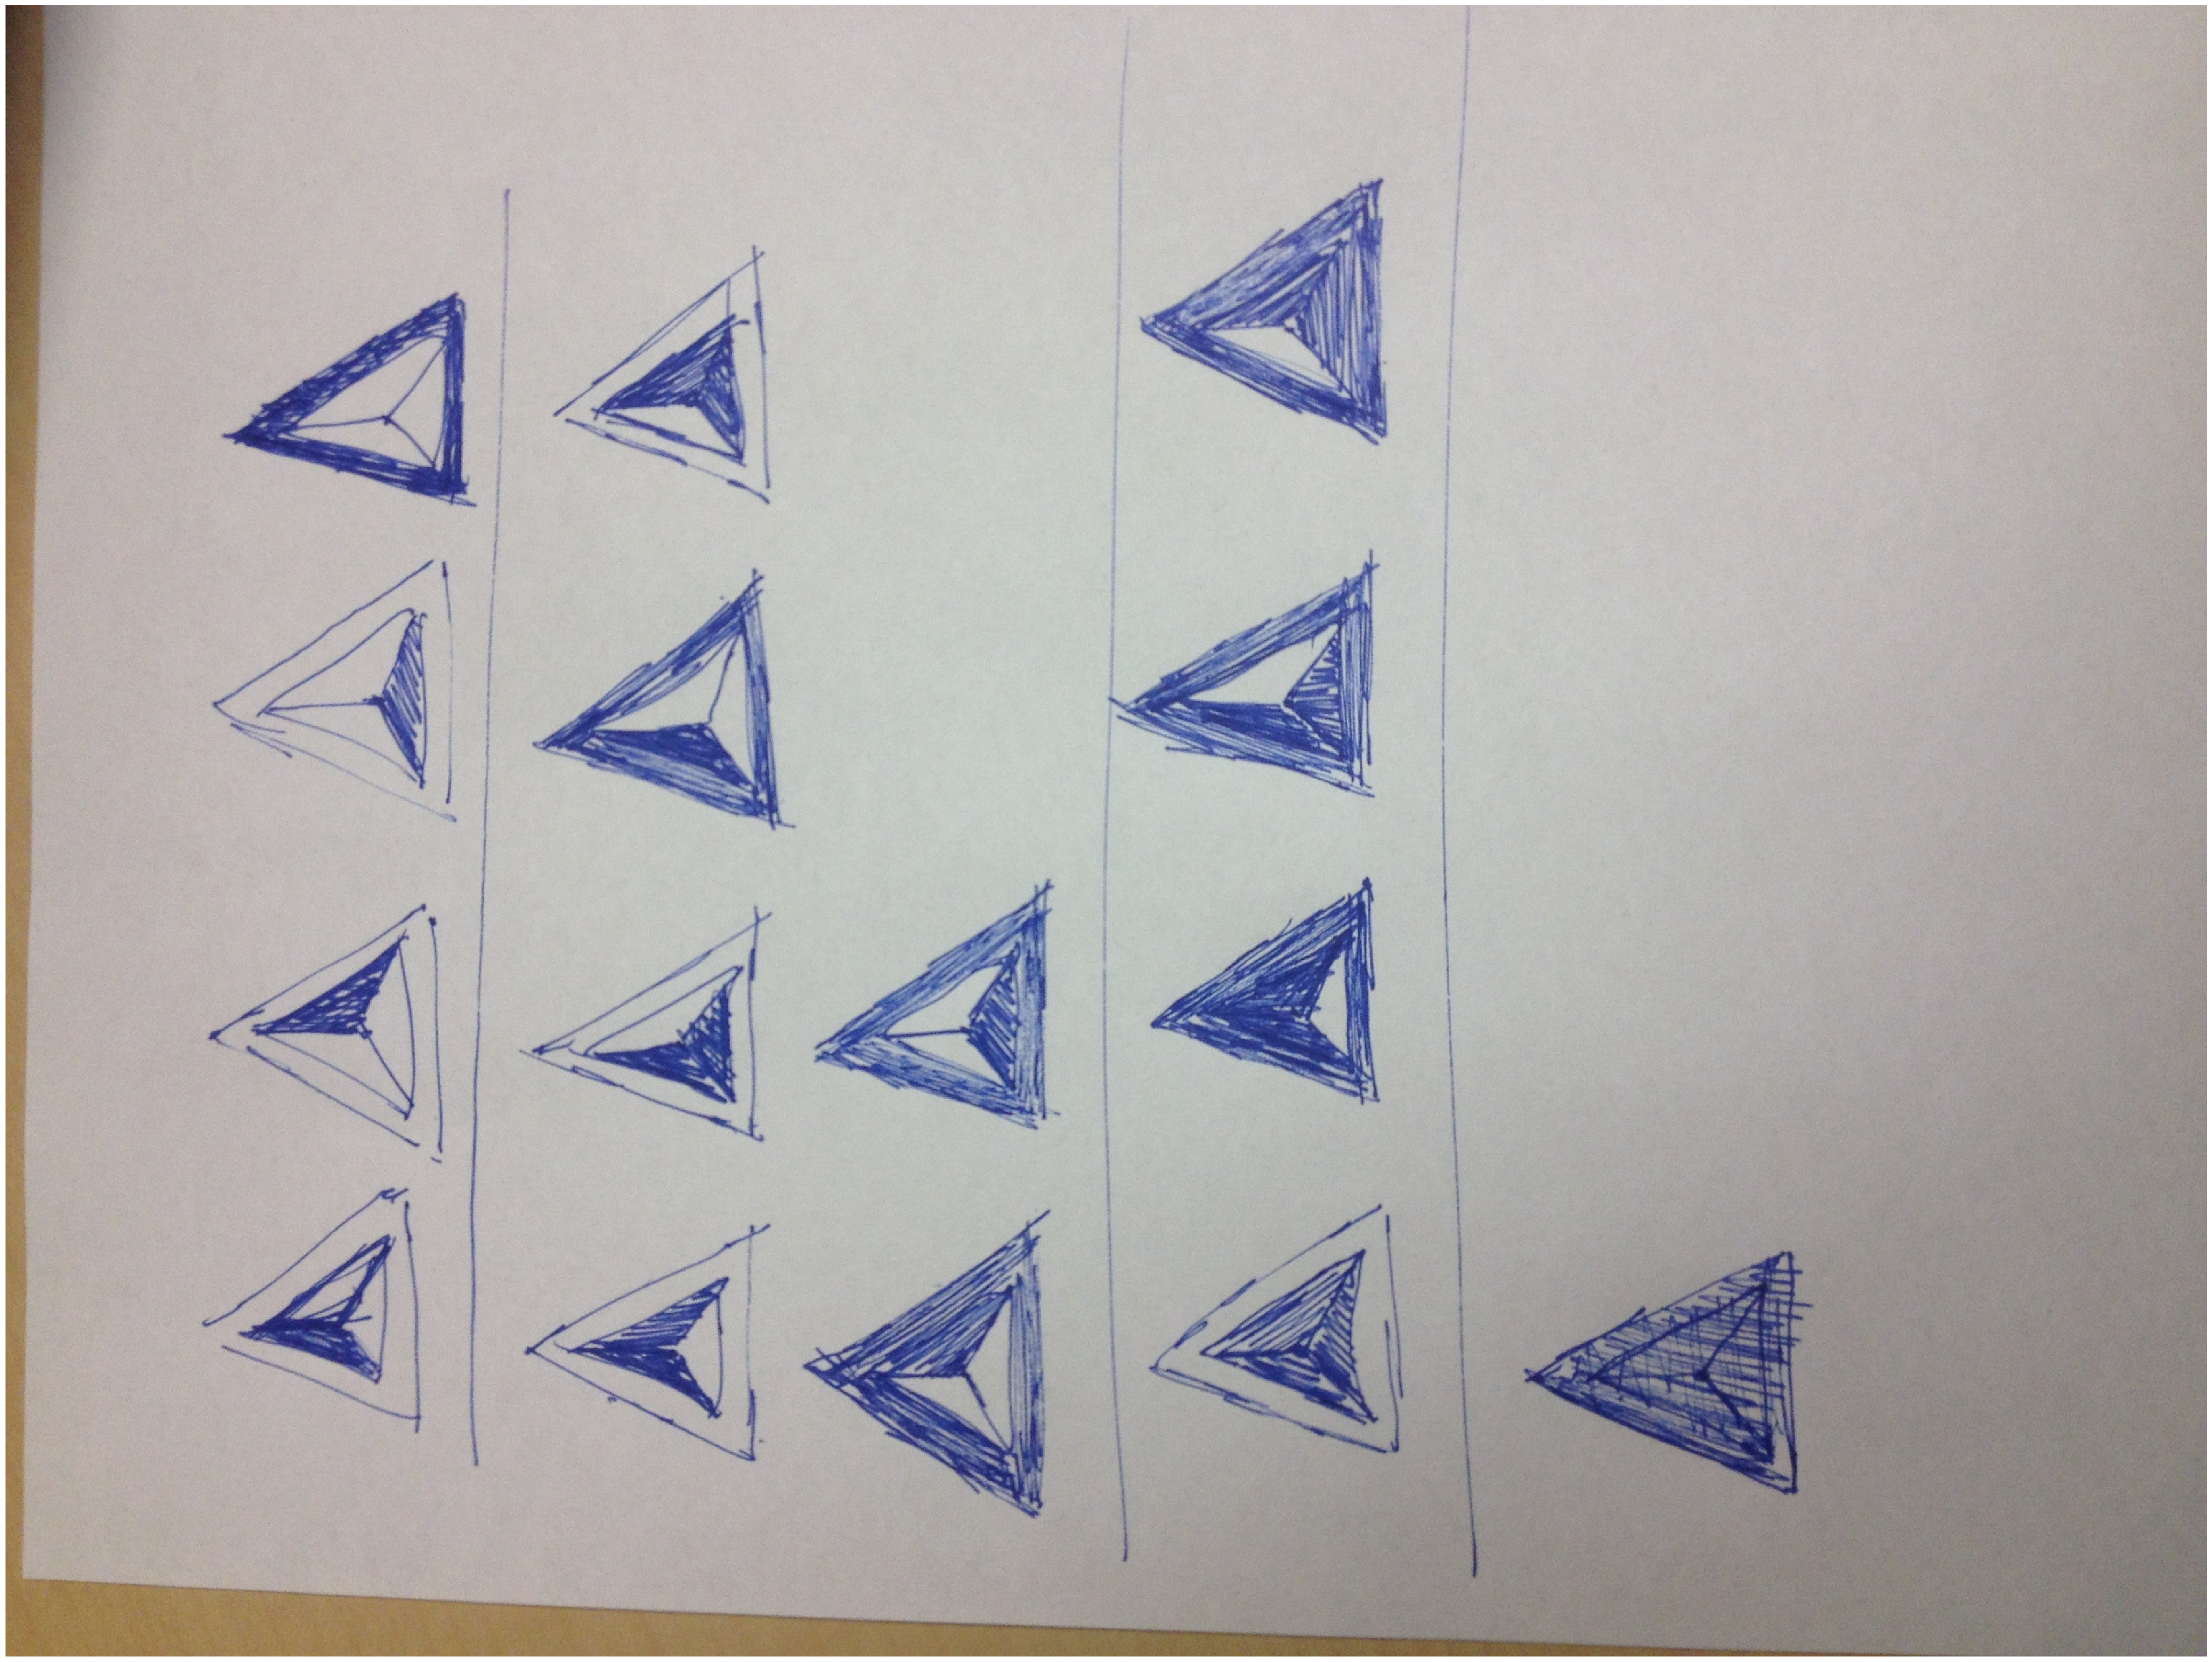
\includegraphics[scale=0.1, angle=0]{tetrahedron_states.eps}
\caption{The building game states of the tetrahedron.}
\label{fig:TetraStates}
\end{figure}
As pictured in figure~\ref{fig:OctaStates}, some subsets of faces are not states. For instance, the subset of octahedron faces with only two faces that are not adjacent is not a state. Similarly, the subset of two faces meeting only at a vertex is not a state as they are not connected through edge adjacency in the graph $\PolyGraph$. However, when more faces are added to connect these faces in $\PolyGraph$ the subset is indeed a state.

\begin{figure}[ht]
  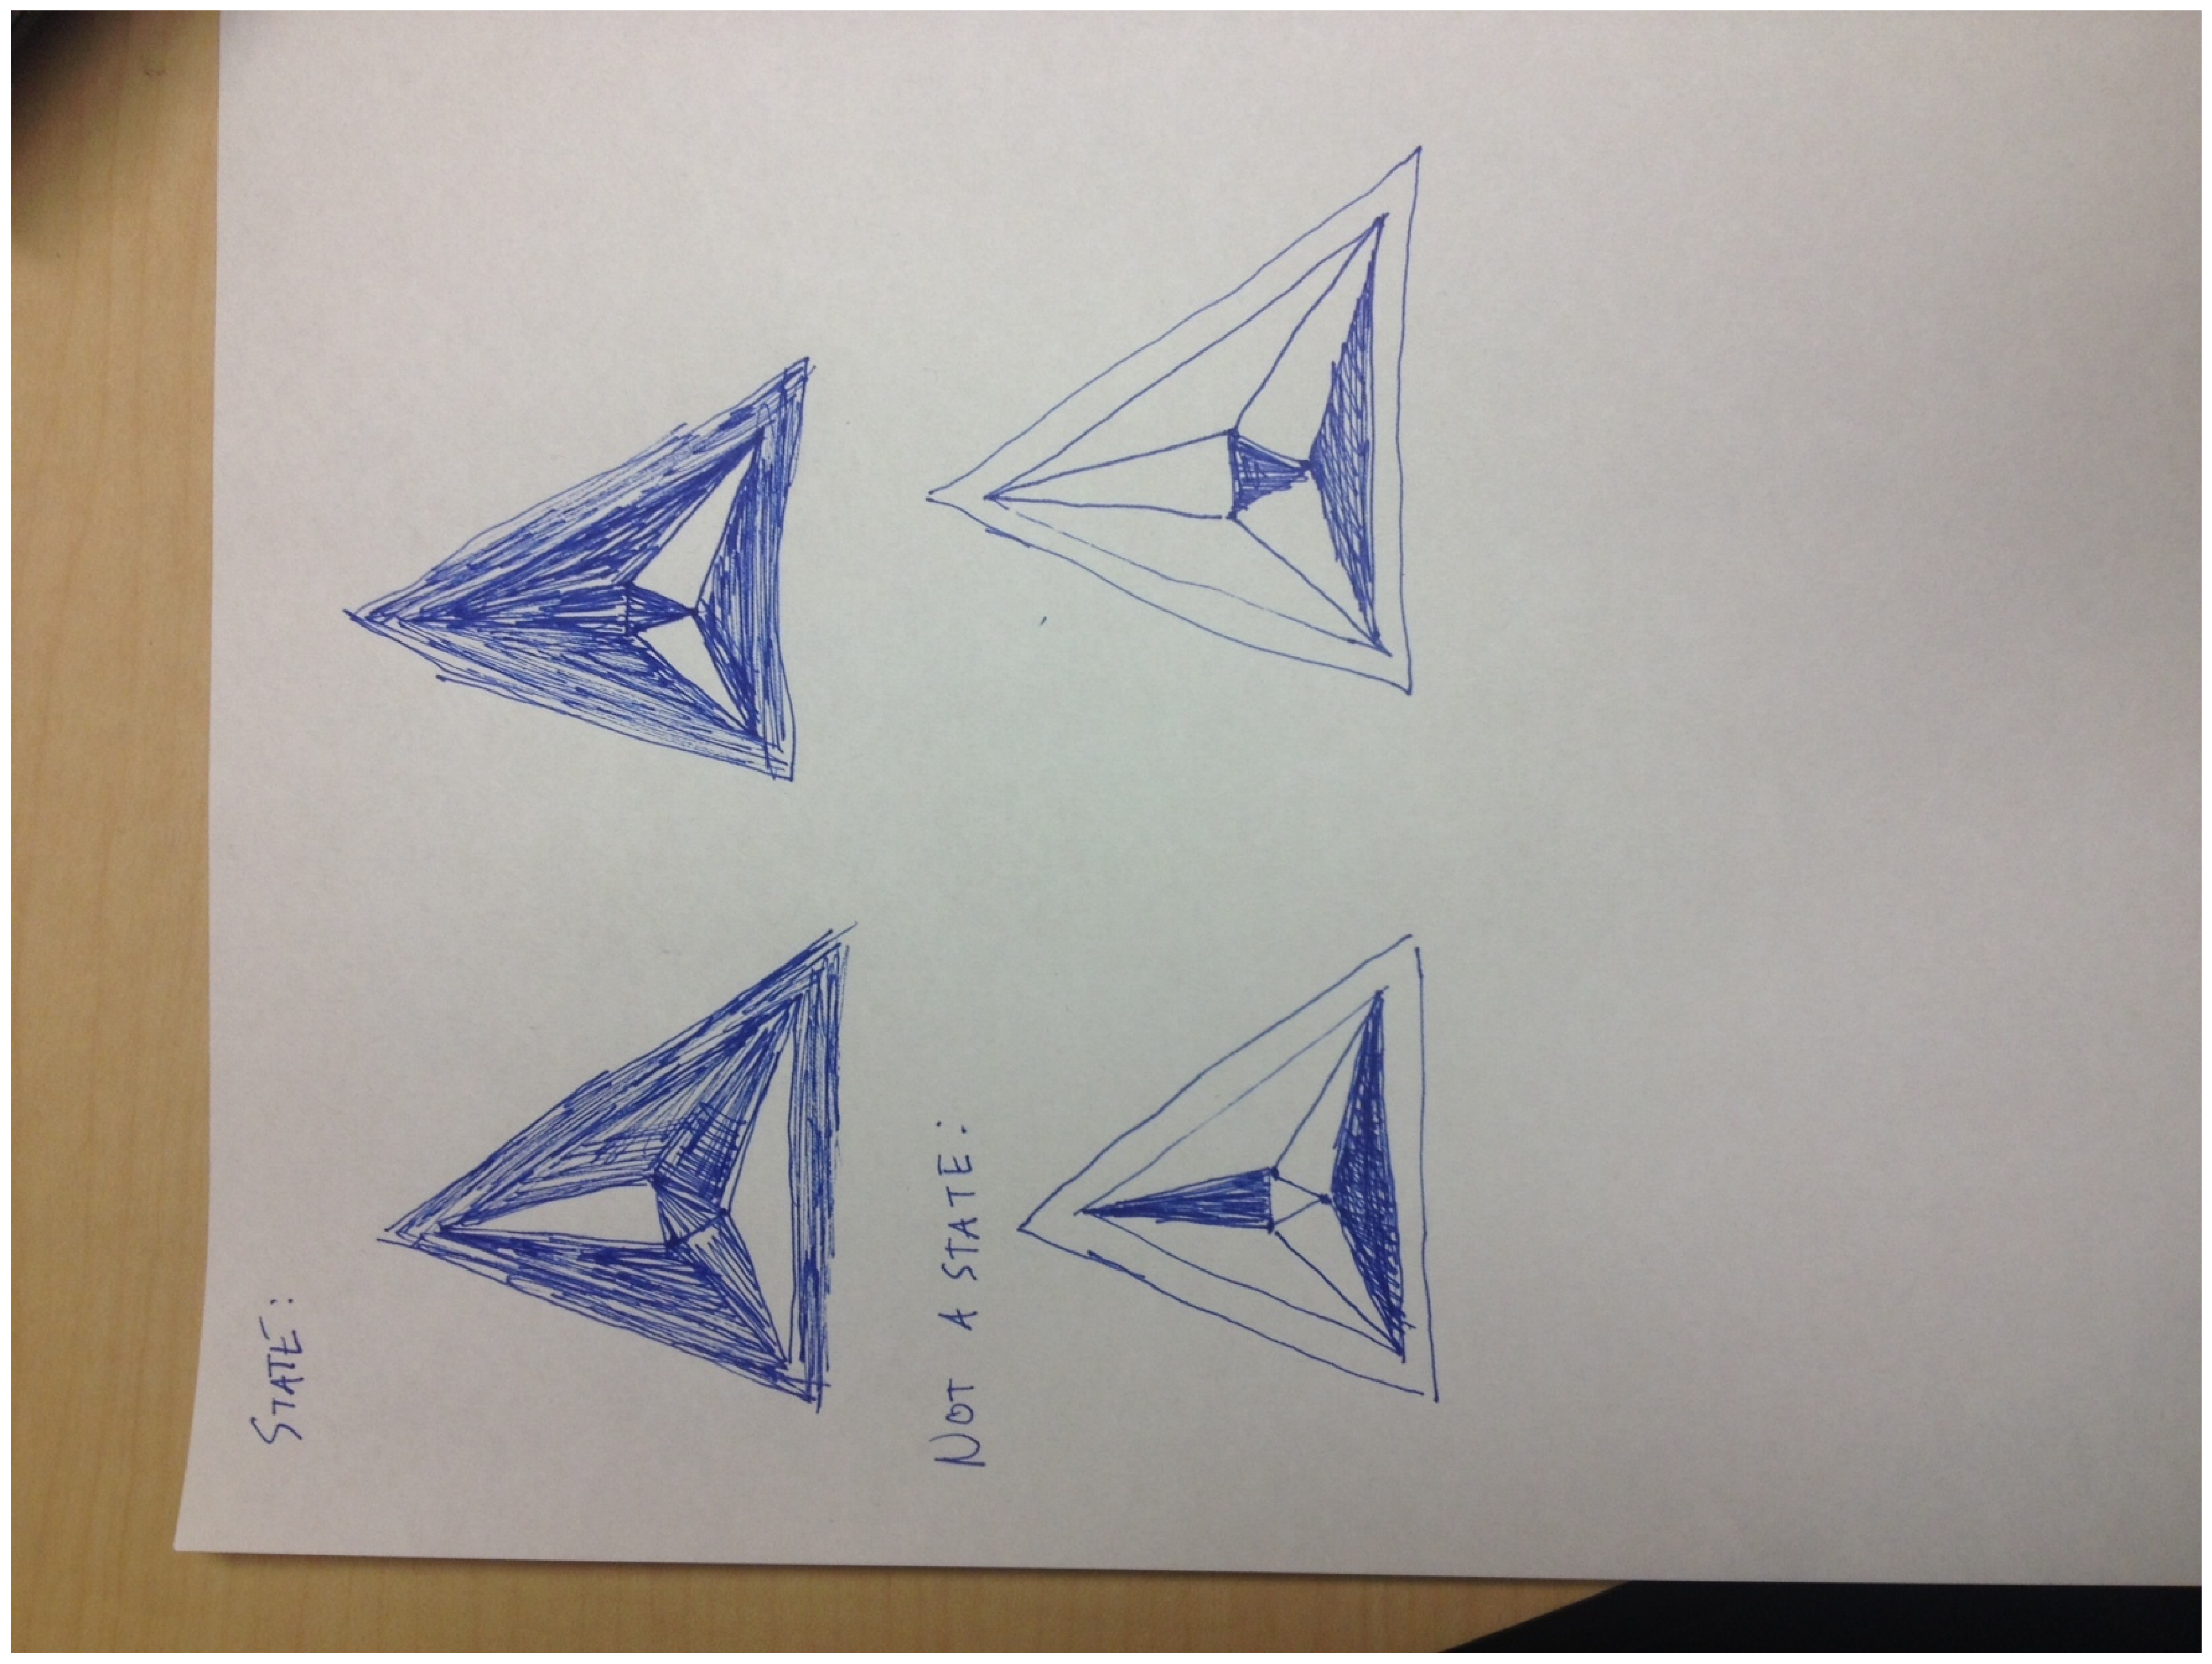
\includegraphics[scale=0.2, angle=0]{octa_state_or_not.eps}
\caption{Examples of octahedron states and non-states.}
\label{fig:OctaStates}
\end{figure}
 


%as a sequential graph labeling process. If we are interested in the BG of a polyhedron \poly, we represent \poly\spc by a graph $\PolyGraph = \left(F, E\right)$ whose nodes are the faces $F$ of \poly\spc and connections $E$ correspond to the pairs of faces sharing an edge of \poly. In this way, $\PolyGraph$ can be viewed as the polyhedral graph of \poly's dual polyhedron. 
 
%In Zlotnick's usage of the model, the labeling of $1$ or $0$ to each face would correspond to whether the face had been attached at some point up to the current step of the process. 

%--More describing fig and what is and is not an intermediate.

%The corresponding $\PolyGraph$ representation is the octahedral graph with 6 vertices and 12 edges. In this example, the state represented labels three faces with a 1 and the others with 0. The embedded geometric interpretation shows three square faces connected along their edges.

%\begin{figure}[ht]
%  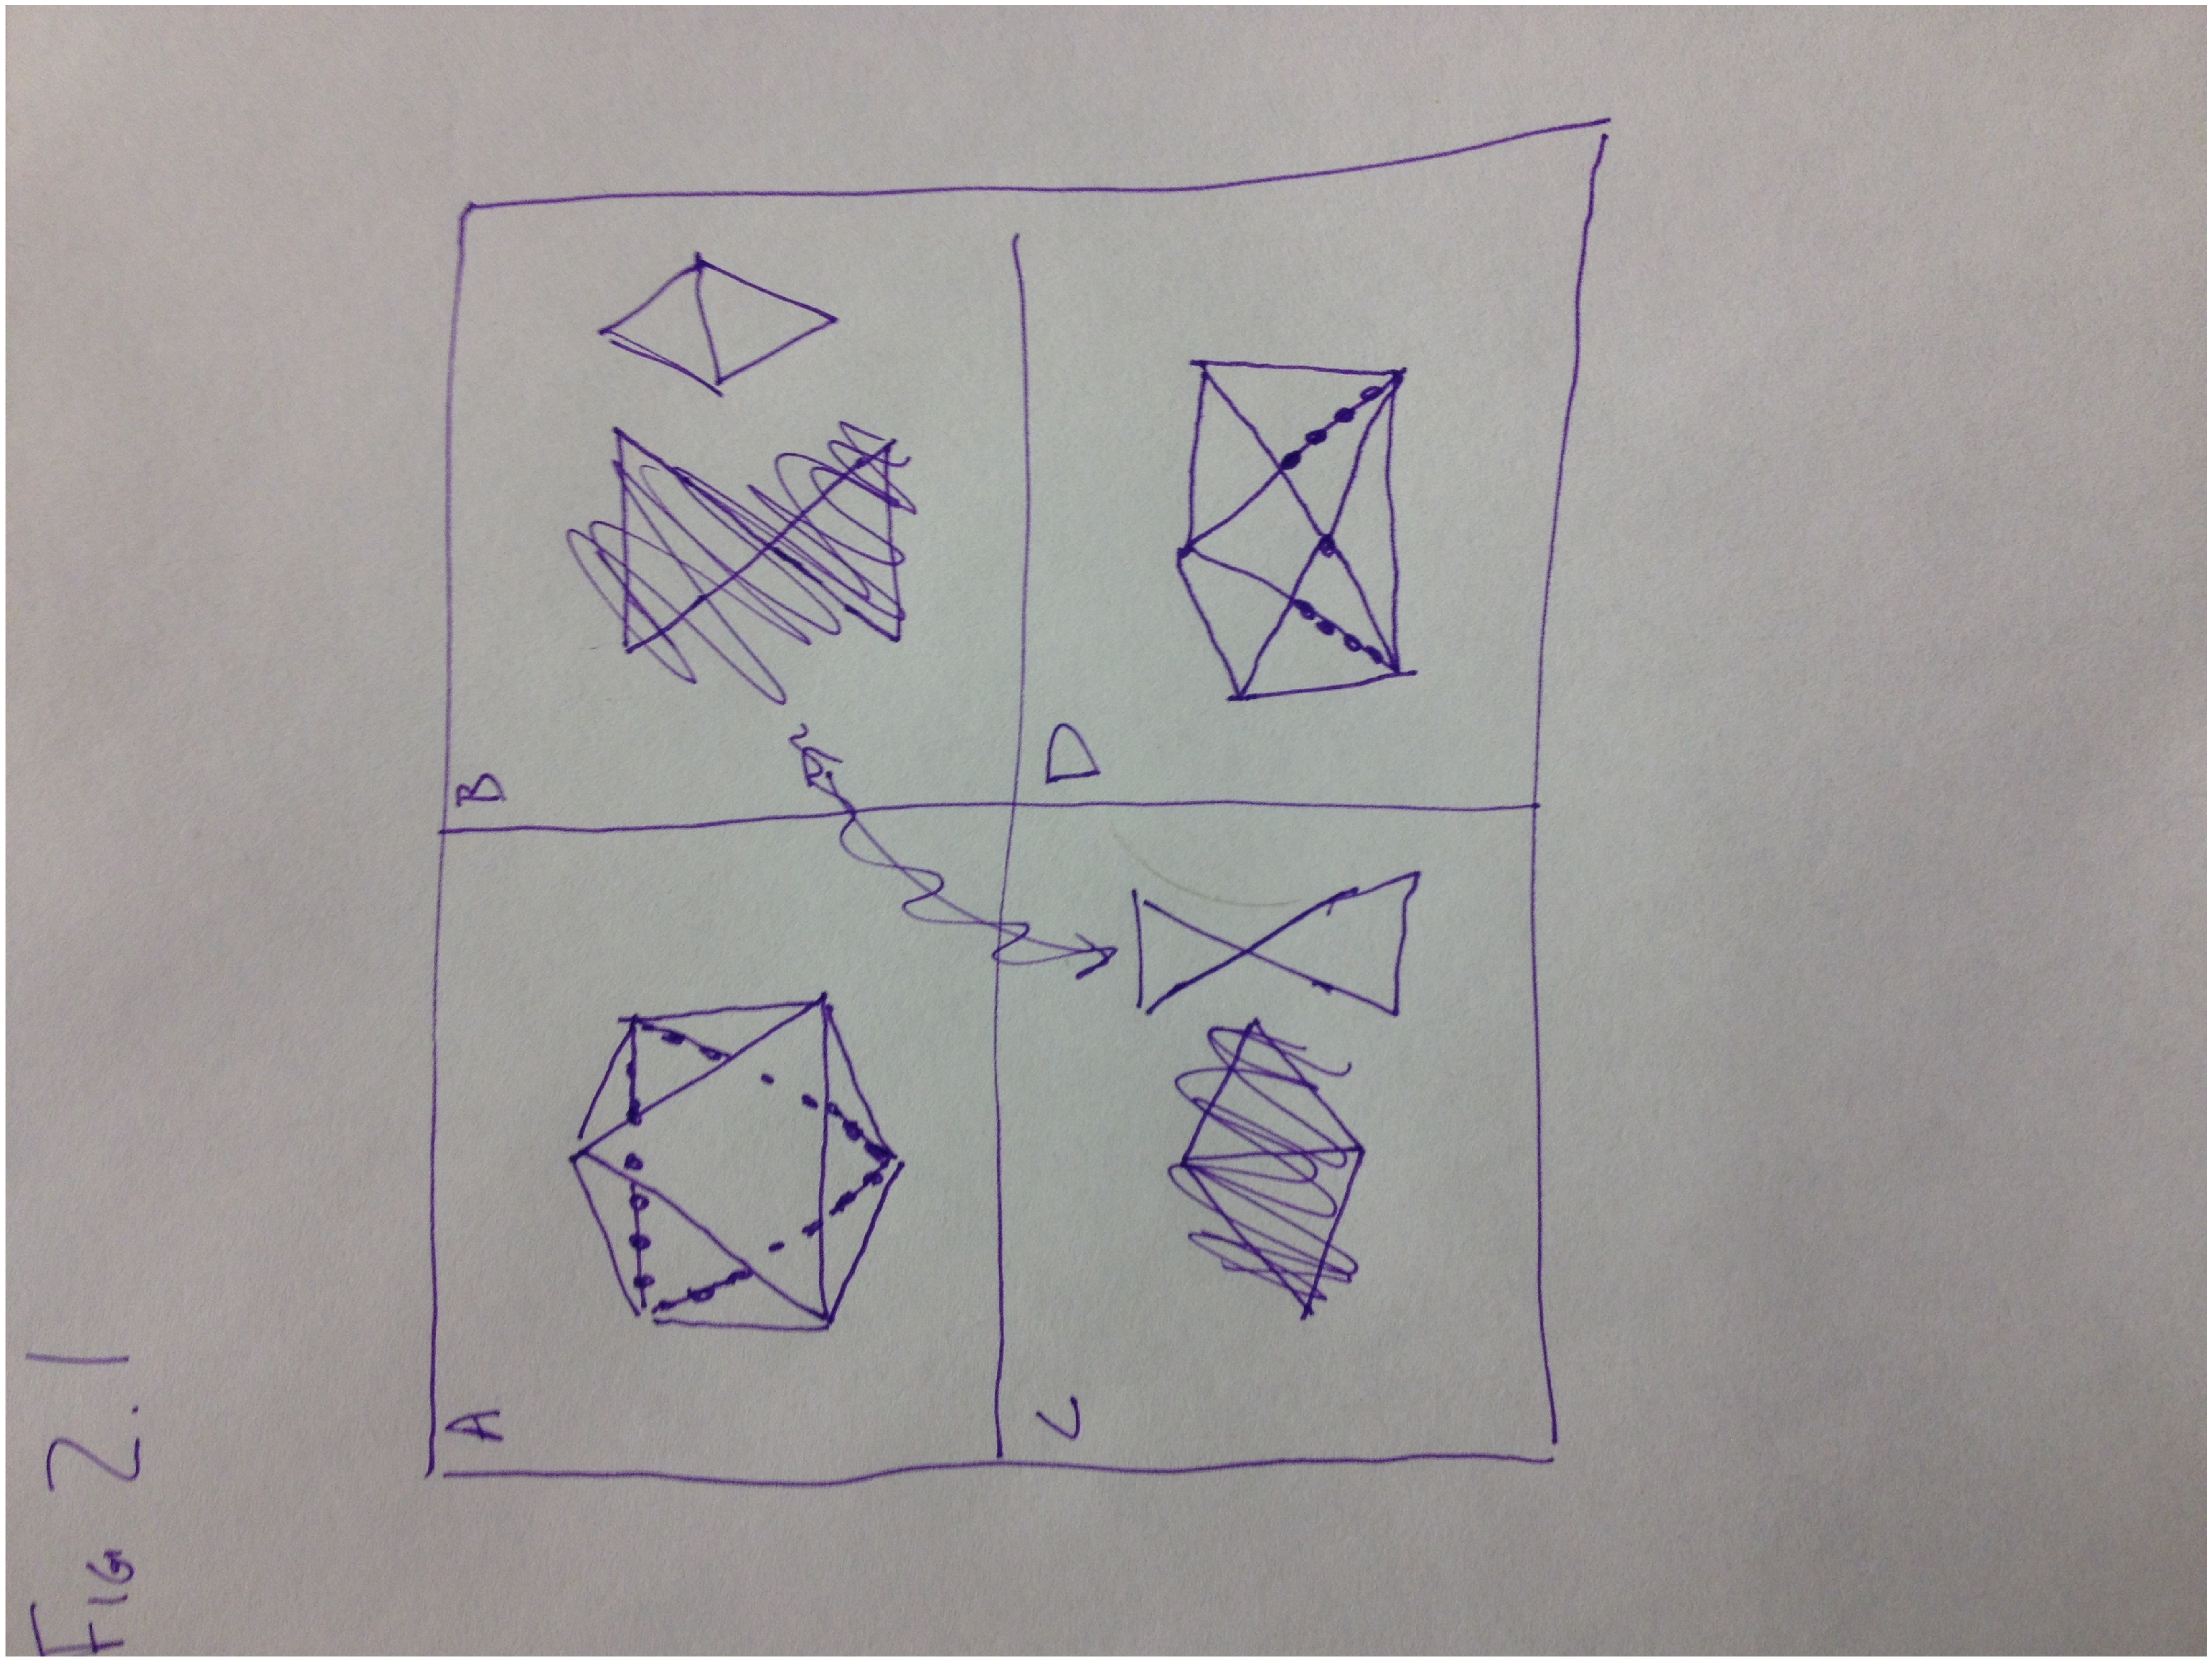
\includegraphics[scale=0.1, angle=0]{fig_2_1.eps}
%\caption{The cube and its graph representation.}
%\label{fig:OctaStates}
%\end{figure}

%\begin{mydef}
%The Building Game \textbf{rotation group} $\G$ is the permutation group acting on $F$ that corresponds to \poly's rotational symmetry group.
%\end{mydef}


\subsection{Group Actions}

It is easy to see that many states are combinatorially equivalent and are just rotations of each other. As in Zlotnick, we group the states into sets that are rotations of each other. However, to do so, we must first build the mathematical infrastructure using group actions. 

\begin{mydef}%[~\cite{Rotman1995} CITE]
A \textbf{group action} of a group $G$ on a set $X$ is a function mapping $G \times X$ to $X$ with $(g\in G, x \in X) \mapsto g.x$ that satisfies: (i) $(gh).x = g.(h.x)$ for $g,h \in G$ and (ii) $e.x = x$ for $e$ the identity element of $G$.
\end{mydef}

We typically use a polyhedron's rotation group or one of its subsgroups as $G$ and $2^F$, the set of subsets of $F$ as the set $X$ that $G$ acts on. In this case, the action $g.x$ permutes the faces of the polyhedron according to the element $g$ of the rotation group and results in a new subset of faces. Here, we introduce the group action concepts of orbits and stabilizer subgroups as they play an important role in out later analyses. 
\begin{mydef}%[~\cite{Rotman1995}]
Let $G$ be a group acting on a set $X$, the \textbf{orbit} of an element $x \in X$ is the subset $G.x \doteq \left\{g.x : g \in G \right\}$ of $X$~\cite{Rotman1995}.
\end{mydef}
We also use the shorthand notation $[x]$ to refer to the orbit $G.x$ for convenience. 
\begin{mydef}%[~\cite{Rotman1995}]
For a  group $G$ acting on a set $X$, the \textbf{stabilizer subgroup} for an element $x\in X$ is the subgroup $G_x \doteq \left\{g \in \G :g. x = x \right\}$ of $G$ that fixes $x$~\cite{Rotman1995}.
\end{mydef}

---statement of the orbit stabilizer theorem
\begin{mythm}[Orbit-Stabilizer~\cite{Rotman1995}]
Let $G$ be a group acting on a set $X$, then for any $x \in X, |G.x| = [G:G_x]$   
\end{mythm}
\begin{mythm}[Lagrange~\cite{Rotman1995}]
If $G$ is a finite group and $S \leq G$, then $|S|$ divides $|G|$ and $[G:S] = |G|/|S|$
\end{mythm}
\begin{mylem}[Burnside~\cite{Rotman1995}]
Let $G$ be a finite group acting on a set $X$, then $$|X\G| = \frac{1}{|G|}\sum_{g \in G}|X^g|$$ where $|X/G|$ is the number of orbits and $|X^g| = {x \in X : g.x = x}$ 
\end{mylem}

\begin{mycor}
Let $G$ be a finite group acting on a set $X$, then for any $x \in X$
\begin{align}
|G.x| = \frac{|G|}{|G_x|}.
\end{align}
\end{mycor}
\begin{proof}
This result follows trivially from Lagrange's theorem and the Orbit-Stabilizer theorems. 
\end{proof}


\begin{mydef}
The \textbf{symmetry number} $r_x$ of a state $x$ is the order of its stabilizer subgroup $\left|\G_x\right|$.
\end{mydef}


\begin{figure}[ht]
  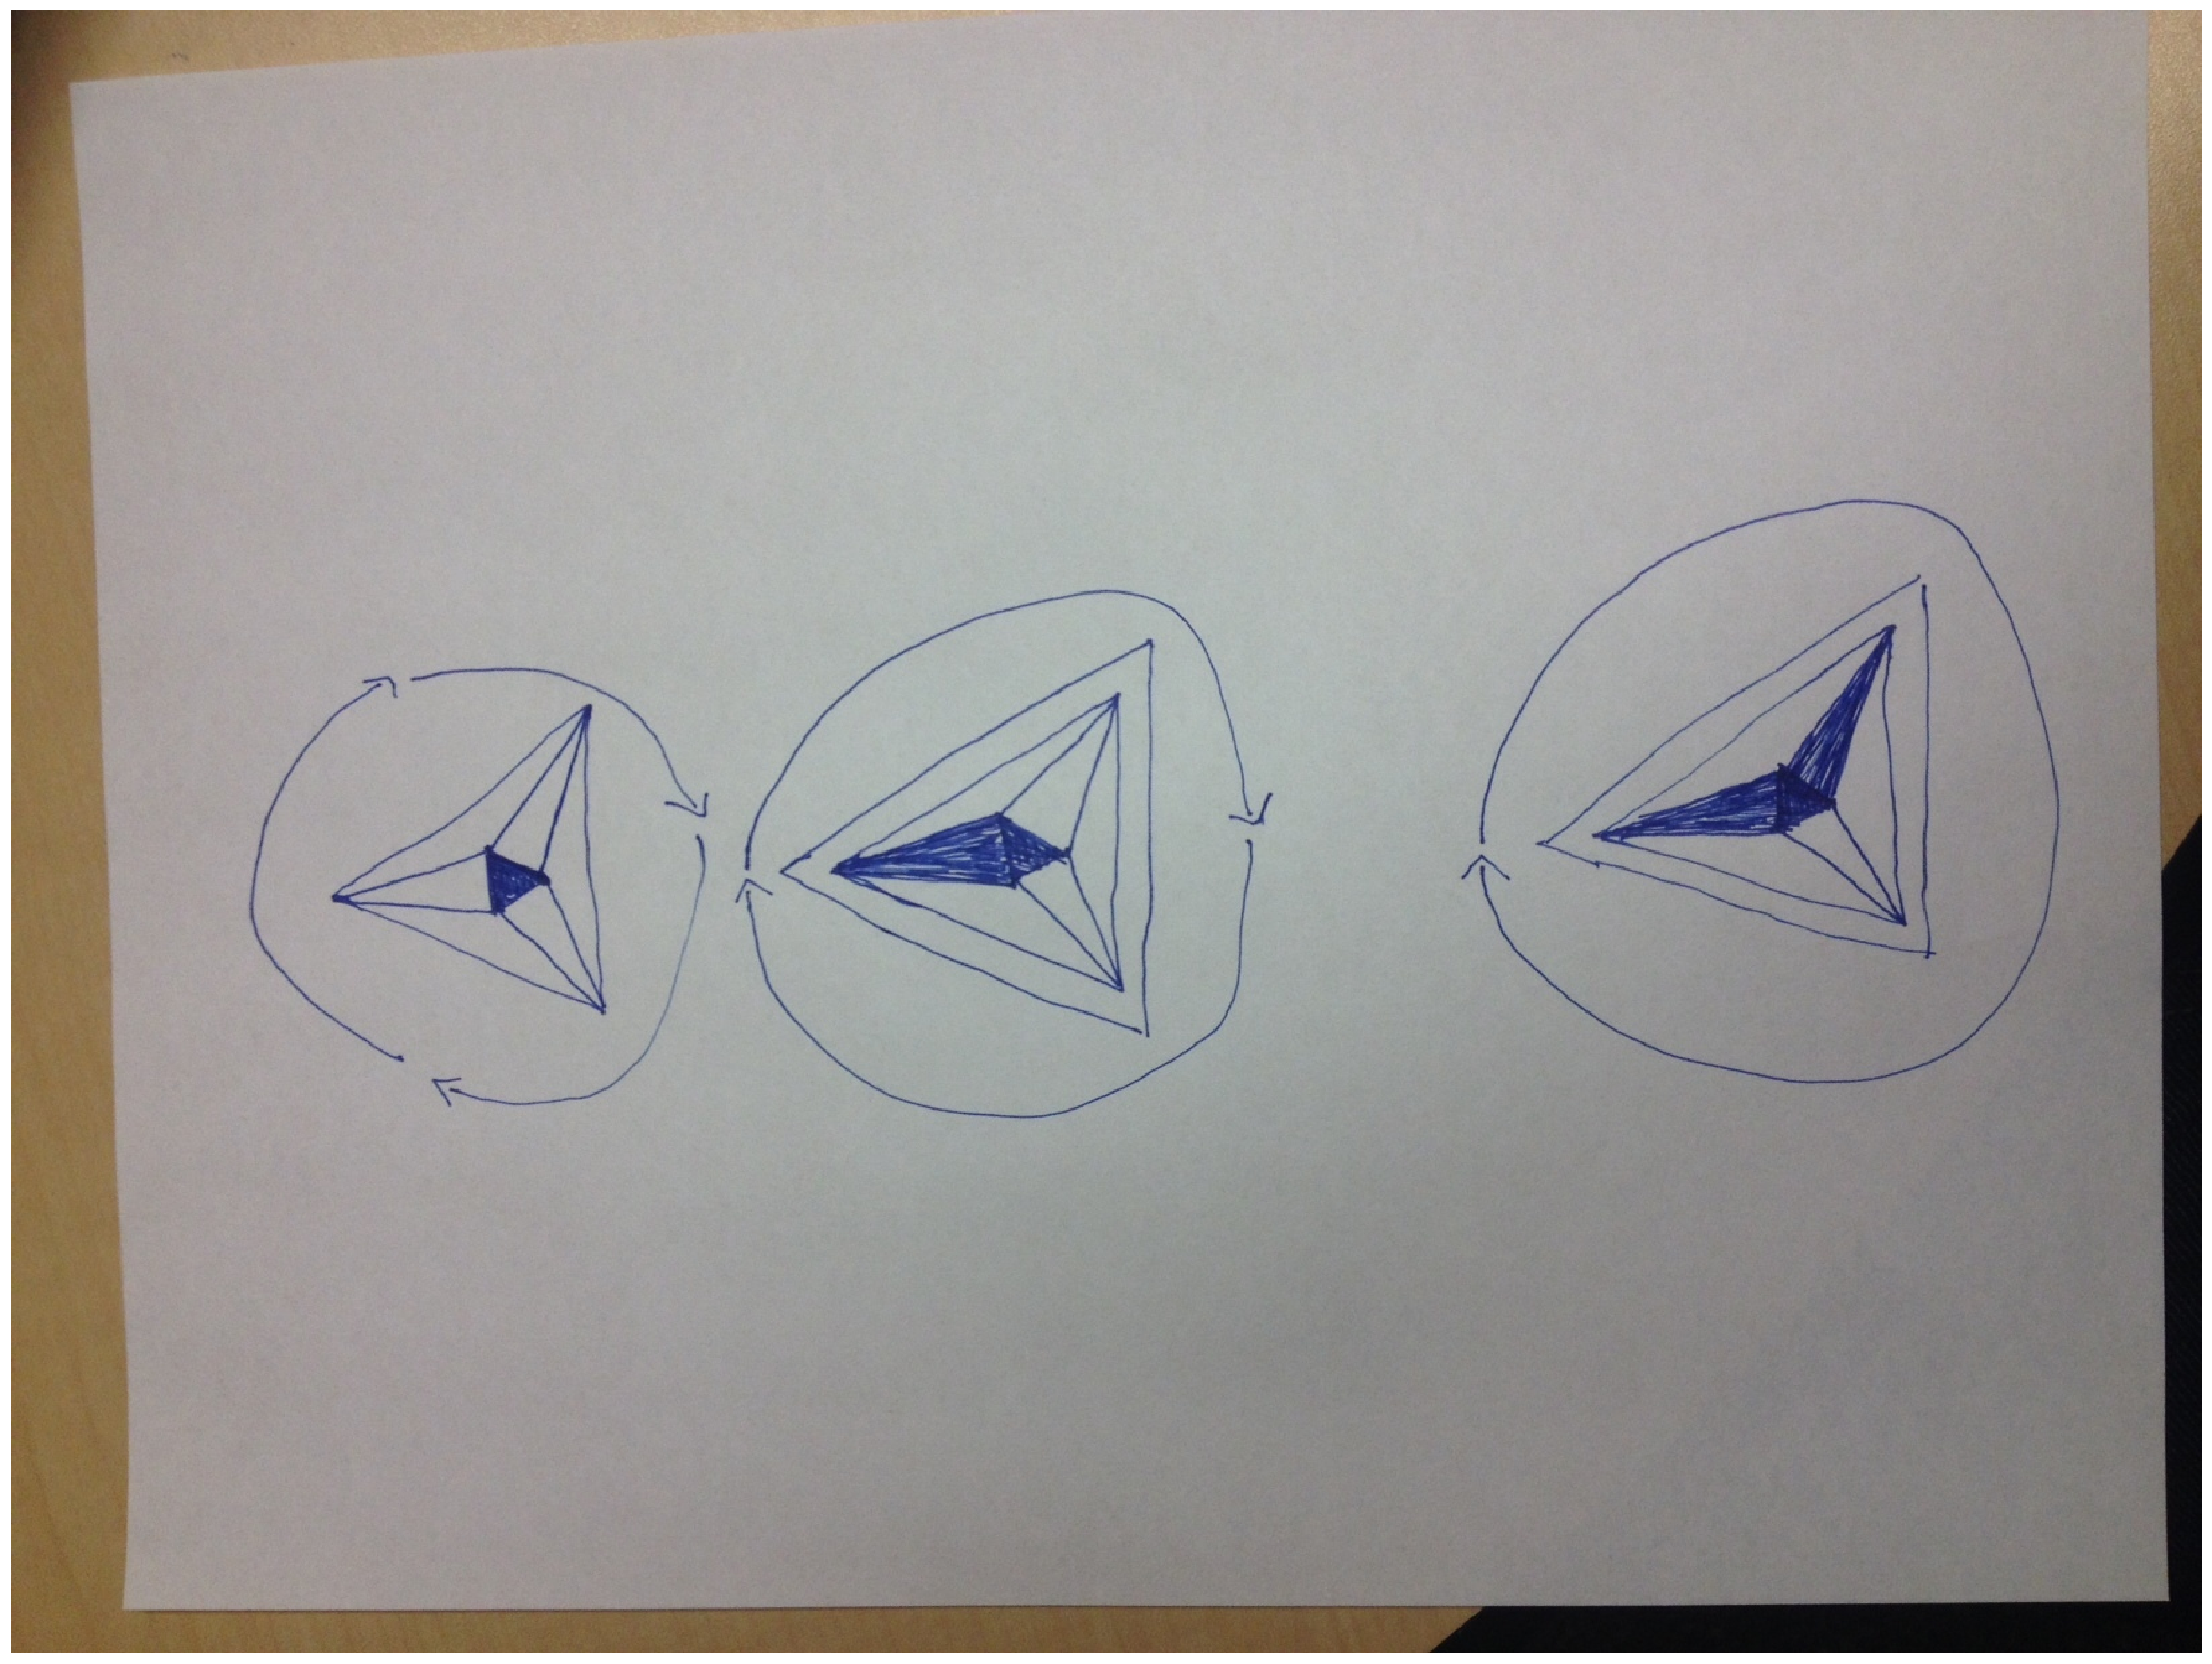
\includegraphics[scale=0.2, angle=0]{octa_stabilizers.eps}
\caption{The stabilizer subgroups for various octahedron states.}
\label{fig:OctaStabs}
\end{figure}
 


\subsection{Building Game Intermediates}


\begin{mydef}
A Building Game \textbf{intermediate} $[x] \doteq \left\{g.x : g \in G\right\}$ is the orbit of the state $x$. 
\end{mydef}
Then, since the orbits of a group action form a partition on the set it acts on, each state belongs to a single intermediate and two states $x$ and $y$ are part of the same intermediate if there is a $g\in\G$ such that $y = g.x$. 


\begin{mylem}
\label{lem:GyhGxh}
Let $x, y \in \left[x\right]$ such that $y = h.x$ for some $h \in G$. Then, $G_y = hG_xh^{-1}$. 
\end{mylem}
\begin{proof}
Since $G$ is normal to itself, we have $G = h^{-1}Gh = hGh^{-1}$.
\begin{align}
  hG_xh^{-1} &= \left\{hgh^{-1} : g \in G_x \right\} \\
  &= \left\{hgh^{-1} : g.x = x, g \in G\right\} \\
  \intertext{Use the transformation $\hat{g} = hgh^{-1}$.}
  &= \left\{\hat{g} : h^{-1}\hat{g}h.x = x, \hat{g} \in hGh^{-1} \right\} \\ 
  &= \left\{\hat{g} : \hat{g}.(h.x) = h.x, \hat{g} \in G \right\} \\ 
  &= \left\{\hat{g} : \hat{g}.y = y, \hat{g} \in G \right\} \\ 
  &= G_y
\end{align}
\end{proof}

\begin{mythm}
If the states $x$ and $\hat{x}$ are members of the same intermediate $\left[x\right]$, they have the same symmetry number. Thus, we extend the notion of a symmetry number to be a property of an intermediate.
\end{mythm}
\begin{proof}
By Lemma~\ref{lem:GyhGxh}, the result follows.
\begin{align}
  r_x &= |G_x| \\
  &= |hG_xh^{-1}| \\
   &= |G_{\hat{x}}| \\
  &= r_{\hat{x}}
\end{align}
\end{proof}


%\begin{figure}[ht]
%\caption{The eight states in a particular BG intermediate.}
%\label{fig:CubeState}
%\end{figure}

%For ease of exposition, we use the notational shorthand $\left(x\right)_m$ for $x\left(f_m\right)$ and $x = g.x'$ when $x(f_m) = x'(g.f_m)$ for every $f_m \in F(\mathscr{P})$. Additionally, we denote the intermediate satisfying $\left(x\right)_m = \colorA$ for all $f_m \in \faceset$ as $x^\colorAsm$ and similarly $x^\colorBsm$ is the intermediate with $\left(x\right)_m = \colorB$ for all $f_m \in \faceset$. The function counting the number of \colorB\spc faces an intermediate has is denoted $h\left(x\right) \doteq |\left\{f_m \in \faceset : \left(x\right)_m = \colorB\right\}|$.

\begin{mydef}
Two distinct intermediates $\left[x\right]$ and $\left[y\right]$ are \textbf{connected} if there exist states $x \in \left[x\right]$ and $y \in \left[y\right]$ such that one of the following holds:
\begin{itemize}
\item $\exists f \in y: y = x \cup \left\{f\right\}$
  \item $\exists f \in x: x = y \cup \left\{f\right\}$
\end{itemize}
\end{mydef}

-- Language about forward and backward connection directions?

\begin{mylem}
If intermediates $\left[x\right]$ and $\left[y\right]$ are connected, then for every state $x \in \left[x\right]$ there is a state $y \in \left[y\right]$ such that $\exists f \in y: y = x \cup \left\{f\right\}$ or $\exists f \in x: x = y \cup \left\{f\right\}$.
\end{mylem}
\begin{proof}
  Without loss of generality, assume $|x| < |y|$. Since $[x]$ and $[y]$ are connected, let $\hat{x} \in [x]$, $\hat{y} \in [y]$, and $\hat{f} \in \hat{y}$, be such that $\hat{y} = \hat{x}\cup\{\hat{f}\}$. Then, for any $x \in [x]$, pick $g \in G$ such that $x = g.\hat{x}$. By choosing $y = g.\hat{y}$ and $\{f\} = g.\{\hat{f}\}$, we have
\begin{align}
  y &= g.\hat{y} \\
  &= g.(\hat{x}\cup\{\hat{f}\}) \\
  &= g.\hat{x}\cup g.\{\hat{f}\} \\
  &= x \cup \{f\} \\
\end{align}    
and our result is shown.
\end{proof}


\begin{mydef}
A Building Game \textbf{pathway} is a sequence of intermediates $[x^{p_1}], [x^{p_2}], \dots, [x^{p_N}]$ such that  $[x^{p_i}]$ is connected to $[x^{p_{i+1}}]$, $|x^{p_i}| = i$, and $x^{p_N} = F$.
\end{mydef}

 Figure~\ref{fig:DodecBG} shows a Building Game pathway for the dodecahedron using Schlegel diagrams. The pathway has 12 intermediates since there must be exactly one intermediate $x^{p_i}$ satisfying $h\left(x^{p_i}\right) = i$ for each $i = 1,2,\dots,12$.

\begin{figure}[ht]
\caption{One Building Game pathway on the dodecahedron.}
\label{fig:DodecBG}
\end{figure}

With many pairs of connected intermediates, we organize these relations in a graph.

\begin{mydef}
The Building Game \textbf{combinatorial configuration space} for a polyhedron \poly\spc is a graph in which the nodes are \poly's intermediates and a graph edge exists between two intermediates if and only if they are connected. 
\end{mydef}

When the intermediates are partitioned by the number of faces they possess, it is natural to arrange the state space as a tiered graph according to this partition. Figure~\ref{fig:CubeSS} shows the Building Game state space for the cube. As seen, each tier has intermediates with the same number of faces and connections thus exist with intermediates that are either in the tier directly above or below them. We can also see that there are three distinct pathways contained in the state space. 

\begin{figure}[ht]
\caption{The Building Game combinatorial configuration space of the cube.}
\label{fig:CubeSS}    
\end{figure}

Interestingly, it is not the case that the addition or removal of each face of an intermediate results in a distinct intermediate. 
\begin{mydef}
For two connected intermediates $[x^j]$ and $[x^k]$, the set of different faces $$F_{jk} \doteq \left\{f \notin x^j : x^j\cup\{f\} \in [x^k]\right\}\cup\left\{f \in x^j : x^j\setminus\{f\} \in [x^k]\right\}$$ that can be added or removed from $x^j$ to get an element of $[x^k]$ is called the \textbf{degeneracy set} and the number of such faces $S_{jk} \doteq \left|F_{jk}\right|$ is called the \textbf{degeneracy number}.
\end{mydef}

It is important to note that in general the degeneracy number is not symmetric, i.e. \Sjk$\neq$\Skj\spc for some connections $[x^j] \leftrightarrow [x^k]$ in the state space. Both figures~\ref{fig:DodecBG} and ~\ref{fig:DodecBG} show the forward and backward degeneracy numbers for each connection.

--Add figures mentioned above



%\begin{mythm}
%  For two connected intermediates $[x^j]$ and $[x^k]$, the degeracy numbers $S_{jk}$ and $S_{kj}$ are that same as the cardinality of $G_{x^j}.\{f\}$ and $G_{x^k}.\{f\}$ for $x^j \in [x^j], x^k \in [x^k], f \in F$ satisfying $x^k = x^j \cup \{f\}$.  
%\end{mythm}
%\begin{proof}
%
%First we argue the case of $S_{jk}$ by showing that $G_x^j.\{f\} = \{\hat{f} \in F : x \cup \{\hat{f}\} \in [y]\}$.
%
%Assume $\{\hat{f}\} \in G_{x^j}.\{f\}$. Thus, there is a $g \in G$ such that $g.x = x$ and $g.\{f\} = \{\hat{f}\}$. It follows that
%\begin{align}
%x \cup \{\hat{f}\} &= (g.x)\cup (g.\{f\}) \\
%&= g.(x\cup\{f\}) \\
%&= g.y \in [y].
%\end{align}
%Thus $G_x^j.\{f\} \subset \{\hat{f} \in F : x \cup \{\hat{f}\} \in [y]\}$
%
%Now we assume $\bar{f} \in F$ with $x \cup \{\bar{f}\} \in [y]$ and argue that $\bar{f} \in G_{x^j}.\{f\}$. By lemma XXX we know there is a $h \in G_{x^j}$ such that $x^j \cup \{\bar{f}\} = h.x^k$. It follows that
%\begin{align}
%x^j \cup \{\bar{f}\} &= h.x^k \\
%&= h.(x^j \cup \{f\}) \\
%&= h.x^j \cup h.\{f\}) \\
%&= x^j \cup h.\{f\}) \\
%\end{align}
%and thus $\{\bar{f}\} = h.\{f\}$. This means that $\bar{f} \in G_{x^j}.\{f\}$ and $\{\hat{f} \in F : x \cup \{\hat{f}\} \in [y]\} \subset G_x^j.\{f\}$.
%
%We have shown that $G_x^j.\{f\} = \{\hat{f} \in F : x \cup \{\hat{f}\} \in [y]\}$ and consequently that $S_{jk} = |G_{x^j}.\{f\}|$. The proof for $S_{kj}$ follows similarly.
%\end{proof}



\subsection{Group Theoretic Results}





%Since we define Building Game intermediates as rotationally unique from each other, it is useful to think about the problem in the context of $\mathscr{P}$'s rotational symmetry group $G \doteq G\left(\mathscr{P}\right)$ and group actions. For an intermediate $x^j$, the number of symmetries $r_j$ is the order of the stabilizer subgroup $G_{x^j} \doteq \left\{g \in G : g.x^j = x^j\right\}$ of $G$ that fixes $x^j$. 
%Suppose $x^j$ and $x^k$ are connected in the state space and $\varphi$ is one of the $S_{jk}$ faces that, when added to $x^j$, forms $x^k$. We say $x^j + \varphi = x^k$. The degeneracy number $S_{jk}$ can then be expressed as the order of the orbit $\left(G_{x^j}\right).\varphi$ of $\varphi$ with respect to $x^j$'s stabilizer subgroup. Analogously, we define the reverse degeneracy number as $S_{kj} \doteq \left|\left(G_{x^k}\right).\varphi\right|$

\begin{mylem}
Let $g \in G$ and $x,y \subset F$. Then $g.(x\cup y) = g.x \cup g.y$
\end{mylem}
\begin{proof}
Let $f \in g.(x\cup y)$. Then $g^{-1}.\{f\} \in x \cup y$. Without loss of generality, assume $g^{-1}.\{f\} \in x$. It follows that $f \in g.x$ and $f \in g.x \cup g.y$ as well. Therefore, $g.(x\cup y) \subset g.x \cup g.y$.

Conversely, suppose $\hat{f} \in g.x \cup g.y$ and without loss pick $\hat{f}$ to be in $g.x$. It follows that $g^{-1}.\{\hat{f}\} \in x, x \cup y$ and subsequently $\hat{f} \in g.(x \cup y)$. From this we have the reverse relation $g.x \cup g.y \subset g.(x\cup y)$ which proves our equality.
\end{proof}


\begin{mylem}
\label{lem:I}
Let the Building Game intermediates $[x^j]$ and $[x^k]$ be connected in the combinatorial configuration space. Given $x^j \in [x^j]$, $x^k \in [x^k]$ and $f \in F$ such that $x^k = x^j \cup \left\{f\right\}$, the stabilizer subgroups $G_{x^j,\{f\}} = G_{x^k,\{f\}} = G_{x^j,x^k}$ are all equal.
\end{mylem}
\begin{proof}
\begin{align}
G_{x^k,\{f\}} &= \left\{g \in G : g.x^k = x^k, g.\{f\} = \{f\} \right\} \\
           &= \left\{g \in G : g.(x^j \cup \{f\}) = x^j \cup \{f\}, g.\{f\} = \{f\} \right\} \\
           &= \left\{g \in G : g.x^j \cup g.\{f\} = x^j \cup \{f\}, g.\{f\} = \{f\} \right\} \\
           &= \left\{g \in G : g.x^j \cup \{f\} = x^j \cup \{f\}, g.\{f\} = \{f\} \right\} \\
           &= \left\{g \in G : g.x^j  = x^j, g.\{f\} = \{f\} \right\} \\
           &= G_{x^j,\{f\}} \\
&= \left\{g \in G : g.x^j  = x^j, g.\{f\} = \{f\} \right\} \\           
&= \left\{g \in G : g.x^j  = x^j, g.x^j \cup g.\{f\} = x^j \cup \{f\} \right\} \\     
&= \left\{g \in G : g.x^j  = x^j, g.(x^j \cup \{f\}) = x^j \cup \{f\} \right\} \\ 
&= \left\{g \in G : g.x^j  = x^j, g.x^k = x^k \right\} \\ 
&= G_{x^j,x^k}
\end{align}
%--Add prrof that G-xy = G-xf = G-yf???
\end{proof}



\begin{mylem}
For connected intermediates $[x]$ and $[y]$, with $x \cup \{f\} = y$ and $x \cup \{\hat{f}\} \doteq \hat{y}\in [y]$, the stabilizer subgroups $|G_{x,y}|$ and  $|G_{x,\hat{y}}$ satisfy $|G_{x,y}| = |G_{x,\hat{y}}|$. 
\end{mylem}
\begin{proof}
If there is an $h \in G_x$ such that $\{f\} = h.\{\hat{f}\}$, the result follows similar to lemma XXX as $|G_{x,y}| = |hG_{x,\hat{y}}h^{-1}| = |G_{x,\hat{y}}|$.

However, if $\{f\} \neq h.\{\hat{f}\}$ for every $h \in G_x$, THE RESULT STILL NEEDS TO BE PROOVEN. 
--use the fact that such subgroups fix f, so they must be cycles generated by single rotation. --show that if rotation of f by that single element produces [y] then that same rotation of f-hat will too.  
\end{proof}



\begin{mylem}
\label{lem:I}
Let the Building Game intermediates $[x^j]$ and $[x^k]$ be connected in the combinatorial configuration space, the number of orbits $|F_{jk}/G_{x^j}| = |F_{kj}/G_{x^k}|$.
\end{mylem}
\begin{proof}
Let $G_{x^j}.\{f\} \in F_{jk}/G_{x^j}$. Then, since $f \in F_{jk}$ we know that $x^j\cup\{f\} \in [x^k]$ and thus there is a $g \in G$ such that $g.(x^j\cup\{f\}) = x^k$. Since $g.x^j \in [x^j]$, we know that $g.\{f\} \in F_{kj}$. Then, for any $h \in G_{x^k}$ we see that $hg.(x^j\cup\{f\}) = h.x^k = x^k$. This means that $G_{x^k}.(g.\{f\}) \in F_{kj}/G_{x^k}$.

Now, we similarly assume $G_{x^k}.\{\hat{f}\} \in F_{kj}/G_{x^k}$. Then, $x^k \setminus \{\hat{f}\} \in [x^j]$ and there is a $\hat{g} \in G$ such that $\hat{g}.(x^k \setminus \{\hat{f}\}) = x^j$. Therefore, $\hat{g}.\{\hat{f}\} \in F_{jk}$ as $\hat{g}.x^k \in [x^k]$. So, for every $\hat{h} \in G_{x^j}$ we get $\hat{h}\hat{g}.(x^k\setminus\{\hat{f}\}) = \hat{h}.x^j = x^j$. Thus $G_{x^j}.(\hat{g}.\{\hat{f}\}) \in F_{jk}/G_{x^j}$.

Since we have shown that for every orbit in $F_{jk}/G_{x^j}$ there is a corresponding orbit in $F_{kj}/G_{x^k}|$ and vice versa, the total number of orbits in each set must be the same and our result $|F_{jk}/G_{x^j}| = |F_{kj}/G_{x^k}|$ holds.
\end{proof}



\begin{mythm}
\label{thm:J}
For two Building Game intermediates $[x^j]$ and $[x^k]$ are connected in the combinatorial configuration space, $r_kS_{jk} = r_jS_{kj}$.
\end{mythm}
\begin{proof}
Without loss of generality, assume that $[x^j]$ has one fewer face than $[x^k]$ and pick $x^j \in [x^j]$, $x^k \in [x^k]$ and $f \in F$ such that $x^k = x^j \cup \left\{f\right\}$. Then by Burnside lemma, we have the following~\cite{Rotman1995}. 
\begin{align}
\left|F_{jk} / G_{x^j}\right| &= \frac{1}{|G_{x^j}|}\sum_{g \in G_{x^j}}|(F_{jk})^g| \\
&= \frac{1}{|G_{x^j}|}\sum_{\hat{f} \in F_{jk}}|G_{x^j,\{\hat{f}\}}| \\
&= \frac{|G_{x^j,\{f\}}|}{r_j}\sum_{\hat{f} \in F_{jk}}1 \\
&= \frac{|G_{x^j,\{f\}}|S_{jk}}{r_j}
\end{align}
Then, by lemmas XXX and YYY we have,
\begin{align}
\frac{r_j}{S_{jk}} &= \frac{|G_{x^j,\{f\}}|}{\left|F_{jk} / G_{x^j}\right|} \\
&= \frac{|G_{x^k,\{f\}}|}{\left|F_{kj} / G_{x^k}\right|} \\
&\doteq \frac{r_k}{S_{kj}} 
\end{align}
and the result $r_kS_{jk} = r_jS_{kj}$ follows.
% Then, by the orbit-stabilizer theorem, Lagrange's Theorem and lemma~\ref{lem:I} we have the following~\cite{Rotman1995}.
%\begin{align}
%\frac{r_j}{S_{jk}} &\doteq \frac{\left|G_{x^j}\right|}{\left|\left(G_{x^j}\right).\{f\}\right|} \\
%                   &= \left[G_{x^j} : \left(G_{x^j}\right).\{f\} \right] \\
%                   &= \left|G_{x^j,\{f\}}\right| \\
%                   &= \left|G_{x^k,\{f\}}\right| \\
%                   &= \left[G_{x^k} : \left(G_{x^k}\right).\{f\} \right] \\
%                   &= \frac{\left|G_{x^k}\right|}{\left|\left(G_{x^k}\right).\{f\}y\right|} \\
%                   &\doteq \frac{r_k}{S_{kj}} 
%\end{align}
%The result $r_kS_{jk} = r_jS_{kj}$ follows.
\end{proof}


\section{Stochastic Modeling Results}

Since the Building Game is a sequential process with several choices at each step, it is natural to consider it as a stochastic process. By putting a distribution on all possible faces that can be added or removed at each step of the Building game, a distribution on the space of pathways is implicitly defined. Thus, for a choice of this transition rule, we can ask questions about the likelihood of the different pathways. 

--Math and graphical results about putting a distribution on pathways


If we consider a Building Game process that allows faces to be sequentially added or removed, the process consists of transitions from intermediate to intermediate along connections in the combinatorial configuration space. By specifying a distribution on these transitions, it will induce a stationary measure on the state space.  

We define the Markov process $X_t$ by the transition rate matrix $Q$, with the heuristic that the rate of transition to an intermediate $[x^k]$ from an intermediate $[x^j]$ should be proportional to the number of faces that can be added or removed from $[x^j]$ to reach $[x^k]$. For this reason, we include the degeneracy number $S_{jk}$ as a factor in the transition rate matrix. Furthermore, we model the process using an energetic interpretation in which each intermediate has an energy and to transition between intermediates, an energy barrier $E_{jk} = E_{kj}$ must be overcome. 
%\begin{align}
%\label{eq:TransitionProbability}
% P_{jk} = \frac{1}{z_j}S_{jk}\rh 
%\end{align}
%\begin{align}
%\label{eq:TransitionRate}
%\begin{align}
%$$Q_{jk} = 
\[
  Q_{jk} =
  \begin{cases}
   S_{jk}e^{-\beta\left(E_{jk} - E_{j}\right)} & \text{if } [x^j] \leftrightarrow [x^k]  \\
   -z_j       & \text{if } j = k \\
   0 & \text{else}
  \end{cases}
\]
Here, $z_j \doteq \sum_{\ell: \ell \neq j} S_{j\ell}e^{-\beta\left(E_{j\ell} - E_j\right)}$ is the rate at which the process leaves \xj. 

\subsection{Stationary Distribution}

\begin{mythm}
\label{thm:StatDist}
If the transition rate matrix $Q$ can be decomposed as $Q = DC$ where $D$ is diagonal with each entry of the diagonal positive and $C$ is a symmetric matrix with the non-diagonal entries $C_{jk} > 0$ if and only if $[x^j]$ and $[x^k]$ are connected and $C_{jk} = 0$ if they are not, then $X_t$ has the unique stationary distribution $\pi = \diag\left(D^{-1}\right)$.         
\end{mythm}
\begin{proof}
First, we show $Q$ and $\pi$ satisfy detailed balance.
\begin{align}
\pi_jQ_{jk} &= \left(\frac{1}{D_{jj}}\right)\left(D_{jj}C_{jk}\right) \\
&= C_{jk} \\
&= C_{kj} \\
&= \left(\frac{1}{D_{kk}}\right)\left(D_{kk}C_{kj}\right) \\
                    &= \pi_kQ_{kj}
\end{align}

-- Prove aperiodicity 
-- Prove positive recurrence

\end{proof}


\begin{mythm}
\label{thm:E}
The Markov process $X_t$ defined by the transition rate matrix $Q$ in equation~\ref{eq:TransitionRate} admits the unique stationary distribution $\frac{1}{zr_j}e^{-\beta E_j}$ where $z \doteq \sum_\ell \frac{1}{r_\ell}e^{-\beta E_\ell}$ is the partition function. 
\end{mythm}
\begin{proof}
We take $C_{jk} \doteq \frac{S_{jk}}{zr_j}e^{-\beta E_{jk}}$ and notice that it is symmetric by theorem~\ref{thm:J}. With $D_{jj} \doteq zr_je^{\beta E_j}$ we have our partition.  
\begin{align}
Q_{jk} &= S_{jk}e^{-\beta\left(E_{jk} - E_j\right)} \\
       &= \left(zr_je^{\beta E_j}\right) \left(\frac{S_{jk}}{zr_j}e^{-\beta E_{jk}}\right) \\
       &= D_{jj}C_{jk}    
\end{align}
Thus, by theorem~\ref{thm:StatDist},  $\pi_j = \frac{1}{D_{jj}} = \frac{1}{zr_j}e^{-\beta E_j}$.
\end{proof}


%In order to use theorem~\ref{thm:StatDist} to find the stationary distribution for the transition rule~\ref{eq:TransitionProbability}, we must be able to decompose the degeneracy number \Sjk\spc to fit the template of $\mathbf{C}$ and $\mathbf{D}$. In the following section we derive group theoretic identities to show that this is possible.


\subsection{Hitting Times}

\begin{align}
	\tau^{A}_{j} &\doteq \inf\left\{t \geq 0 : X_t \in A, X_0 = x^j\right\}
\end{align}

\begin{align}
	\nu^{A}_{j} &\doteq \inf\left\{n \geq 0 : Y_n \in A, Y_0 = x^j\right\}
\end{align}

For $j \not\in A$.
\begin{align}
	E\left[\tau^{A}_{j}\right] &= E\left[E\left[\tau^{A}_{j} | Y_1 \right]\right] \\
        &= E\left[ Exp\left(z_j\right) + \tau^{A}_{Y_1} \right] \\
        &=  \frac{1}{z_j} + E\left[\sum_{k}\tau^{A}_{Y_1}\mathbbm{1}_{Y_1 = k}\right] \\
        &=  \frac{1}{z_j} + \sum_{k: k\neq j}E\left[\tau^{A}_{k}\right] P\left(Y_1 = k\right) \\
        &=  \frac{1}{z_j}\left(1 + \sum_{k: k\neq j}q_{jk}E\left[\tau^{A}_{k}\right]\right)     \\
  \sum_{k}q_{jk}E\left[\tau^{A}_{k}\right] &= 1 \\
\end{align}

For $j \in A$.
\begin{align}
	E\left[\tau^{A}_{j}\right] &= 0 \\
\end{align}

As a linear system:
\begin{align}
	\left(\diag\left(\mathbbm{1}_A\right) - \diag\left(\mathbbm{1}_{A^c}\right)Q\right)E\left[\tau^{A}\right] =\mathbbm{1}_{A^c}\\
\end{align}


\begin{align}
\psi_j^A\left(t\right) &\doteq P\left(\tau^A_j \leq t\right) \\
\psi_j^A\left(0\right) &= \mathbbm{1}_{j\in A} \\
\psi_j^A\left(t\right) &= 0 \forall j \in A \\                       
\end{align}

For $j \not\in A$.

\begin{align}
\psi_j^A\left(t\right) &\doteq P\left(\tau^A_j \leq t\right) \\
                       &= \sum_k P\left(\tau^A_j \leq t | Y_1 = x^k\right) P\left(Y_1 = x^k\right) \\ 
                       &= \frac{1}{z_j}\sum_{k: k \neq j} q_{jk} P\left(Exp\left(z_j\right)\tau^A_j \leq t\right)  \\
                       &= \frac{1}{z_j}\sum_{k: k \neq j} q_{jk} \int^t_0 P\left(\tau^A_j \leq t - s\right) z_j e^{-z_j s} ds  \\
                       &= \sum_{k: k \neq j} q_{jk} \int^t_0\psi^A_k\left(t-s\right)e^{-z_j s} ds  \\
                       &= \sum_{k: k \neq j} q_{jk} \int^t_0\psi^A_k\left(r\right)e^{-z_j\left(t-r\right)} dr  \\
e^{z_jt}\psi^A_j\left(t\right) &= \sum_{k: k \neq j} q_{jk} \int^t_0 e^{z_jr}\psi^A_k\left(r\right) dr  \\
e^{z_jt}\frac{d\psi^A_j}{dt} + z_j e^{z_j t} \psi^A_j\left(t\right) &= \sum_{k: k \neq j} q_{jk} e^{z_jt}\psi^A_k\left(t\right)  \\
\frac{d\psi^A_j}{dt} &= \sum_{k} q_{jk} \psi^A_k\left(t\right) 
\end{align}

Combining both cases, we get the linear system and solution.

\begin{align}
        \frac{d\psi^A}{dt} &= \diag\left(\mathbbm{1}_{A^c}\right)Q\psi^A \\
        \psi^A\left(0\right) &= \mathbbm{1}_{A} \\
        \psi^A\left(t\right) &= e^{\diag\left(\mathbbm{1}_{A^c}\right)Qt} \mathbbm{1}_{A} \\ 
\end{align}

This is the solution for the CDF of the stopping time $\tau^A$, but we can also compute the PDF explicitly for $t > 0$.

\begin{align}
        p\left(\tau^A = t\right) &= \frac{d\psi^A}{dt} \\
        &= \diag\left(\mathbbm{1}_{A^c}\right)Q\psi^A
\end{align} 



\clearpage{\pagestyle{empty}\cleardoublepage}

\chapter{The Building Game: Enumeration}
\section{Known Enumerative Results}

When treating the Building Game for a polyhedron as a stochastic process, we must first know what the the combinatorial configuration space is exactly. This is a computational enumeration problem, but the results of this enumeration are also of mathematical interest outside its stochastic use.

Attachment models like the Building Game have been the topic of much research in combinatorial mathematics. A well known example of this is the study of polyominoes. An $n$-omino is a configuration of $n$ attached squares in a $2$-dimensional lattice. As seen in figure~\ref{fig:Tetris}, the classic video game Tetris uses each of the seven rotationally unique tetrominoes ($n = 4$) as game pieces. The enumeration of $n$-ominoes has been extensively studied and there are many enumeration results, both explicit and asymptotic. As in our case, the general goal is to enumerate the polyominoes that are unique when acted on by some group (rotation, reflection, etc) or under certain constraints which are often topological.
\begin{figure}[ht]
  \includegraphics[scale=0.25, angle=0]{images/tetris.eps}
\caption{The seven tetrominoes used in Tetris.}
\label{fig:Tetris}
\end{figure}

The Building Game has a wealth of combinatorial enumeration problems to consider. Some have been addressed in the work of Endres et al.~\cite{Endres2005}. While the original Building Game paper does illustrate many icosahedral intermediates, Wales defines the model differently than we do~\cite{Wales1987}. Another early approach by Zlotnick is more true to our interpretation of the Building Game, but only considers a single pathway and thus is not concerned with enumeration of the entire combinatorial configuration space~\cite{Zlotnick1994}. However in Endres et al., the number of intermediates for each of the Platonic solids is computed. The entire combinatorial configuration space for the dodecahedron and icosahedron is also illustrated~\cite{Endres2005}. 

Before the work of Endres et al, David Wilson enumerated the number of intermediates composed of each number of faces for the icosahedron~\cite{OEIS}. This computation seems to have occurred independent of the scientific context of self-assembly as Wilson's enumerations are referred to as the ``Number of one-sided triangular n-ominoes (or triominoes) on the icosahedron.'' He also includes variants such as the ``Number of triangular n-ominoes on the icosahedron'' which enlarges the equivalence classes to identify intermediate that are reflections of each other. 

\section{New Enumerative Results}

Previous enumeration results for the Building Game have focused on the number of intermediates of the Platonic solids. We extend these results to also count the number of Building Game connections and pathways in the combinatorial configuration space. Additionally, we consider the Platonic, Archimedean, and Catalan solids classes with these results presented in figure~\ref{tab:bgEnum}. 

As we consider polyhedra with more and more faces, there is a combinatorial explosion in the number intermediates in combinatorial configuration space. This was noted in Endres et al., where the dodecahedron has $73$ intermediates and the icosahedron has $2,649$~\cite{Endres2005}. We have enumerated the intermediates for polyhedra of up to $30$ faces in our three classes of polyhedra. The $30$-faced rhombic triacontahdron has the most intermediates of all polyhedra in our computation with $2,423,212$.



%While the 6-faced cube state space has only 8 nodes and 9 nodes, the 20-faced icosahedron state space has 2,649 nodes and 17,241 nodes and the 26-faced truncated cuboctahedron state space has 1,525,605 nodes and 17,672,377. Figure \ref{fig:bgtable} details state space sizes of all polyhedra in the Platonic, Archimedean, and Catalan solid classes of up to 26 faces. 



\begin{figure}[ht]
\scalebox{0.8}{
%{\footnotesize
\centering
%\textbf{Building Game Enumerative Results for the Platonic Solids}
\begin{tabular}{ l | c | r | r | r}
Polyhedra Name & $|F|$ & Intermediates & Connections & Pathways \\
  \hline    
Tetrahedron                     & 4        & 4     	& 3             & 1\\
Cube                            & 6        & 8     	& 9    		& 3\\
Octahedron                      & 8        & 14    	& 21    	& 14\\
Dodecahedron                    & 12       & 73    	& 263   	& 17,696 \\
Icosahedron                     & 20       & 2,649 	& 17,241        & 57,396,146,640\\ \hline
Truncated Tetrahedron           & 8     & 28    	& 63            & 402\\
Cuboctahedron                   & 14  	& 340   	& 1,634         & 10,170,968\\
Truncated Cube                  & 14  	& 499   	& 2,729         & 101,443,338 \\
Truncated Octahedron            & 14  	& 555           & 3,069         & 68,106,377\\
Rhombicuboctahedron             & 26  	& 638,850       & 6,459,801     & 164,068,345,221,515,292,308\\
Truncated Cuboctahedron         & 26  	& 1,525,658     & 17,672,374    & 13,837,219,462,483,379,105,902\\ \hline  
Triakis Tetrahedron             & 12  	& 98            & 318           & 38,938\\
Rhombic Dodecahedron            & 12  	& 127           & 493           & 76,936\\
Triakis Octahedron              & 24  	& 12,748        & 81,296        & 169,402,670,046,670\\
Tetrakis Hexahedron             & 24  	& 50,767        & 394,377       & 4,253,948,297,210,346\\
Deltoidal Icositetrahedron      & 24  	& 209,675       & 1,989,548     & 418,663,242,727,526,726 \\
Pentagonal Icositetrahedron     & 24  	& 345,938       & 3,544,987     & 2,828,128,000,716,774,492\\
Rhombic Triacontahedron         & 30  	& 2,423,212     & 26,823,095    & 161,598,744,916,797,017,978,128\\
\end{tabular}
}
\caption{Building game combinatorial configuration space enumerative results for the Platonic, Archimedean, and Catalan solids.}
\label{tab:bgEnum}
\end{figure}

%--Scatter plot commentary.
\begin{figure}[ht]
\centering
  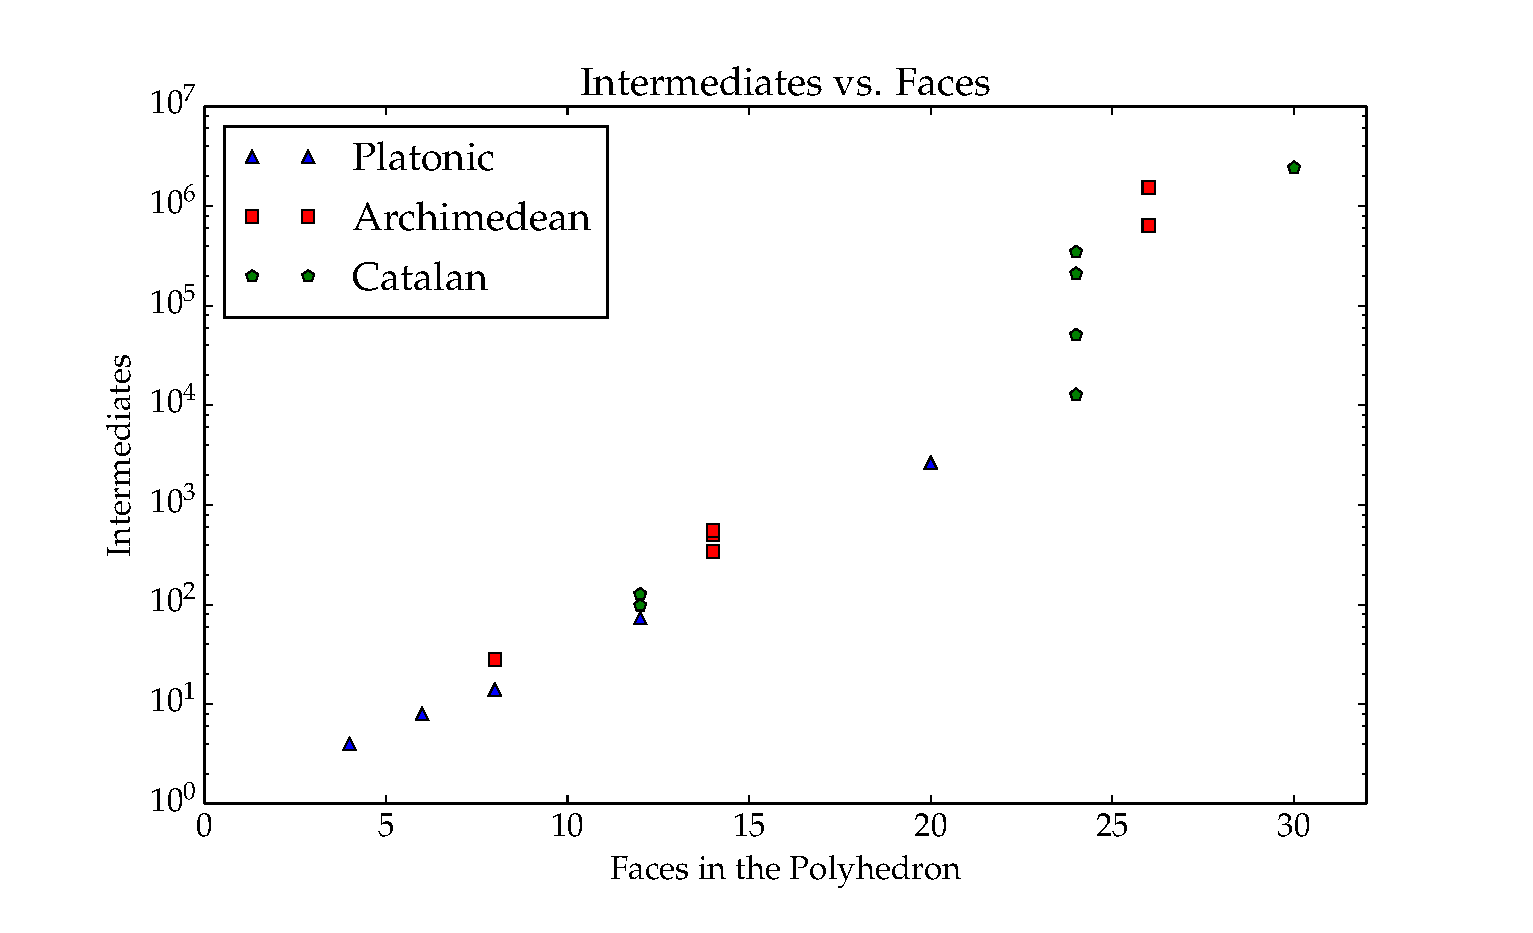
\includegraphics[scale=0.6, angle=0]{images/polys_face_int.eps}
\caption{The relation between number of faces and intermediates in the Building Game combinatorial configuration space.}
\label{fig:FacInt}
\end{figure}

\begin{figure}[ht]
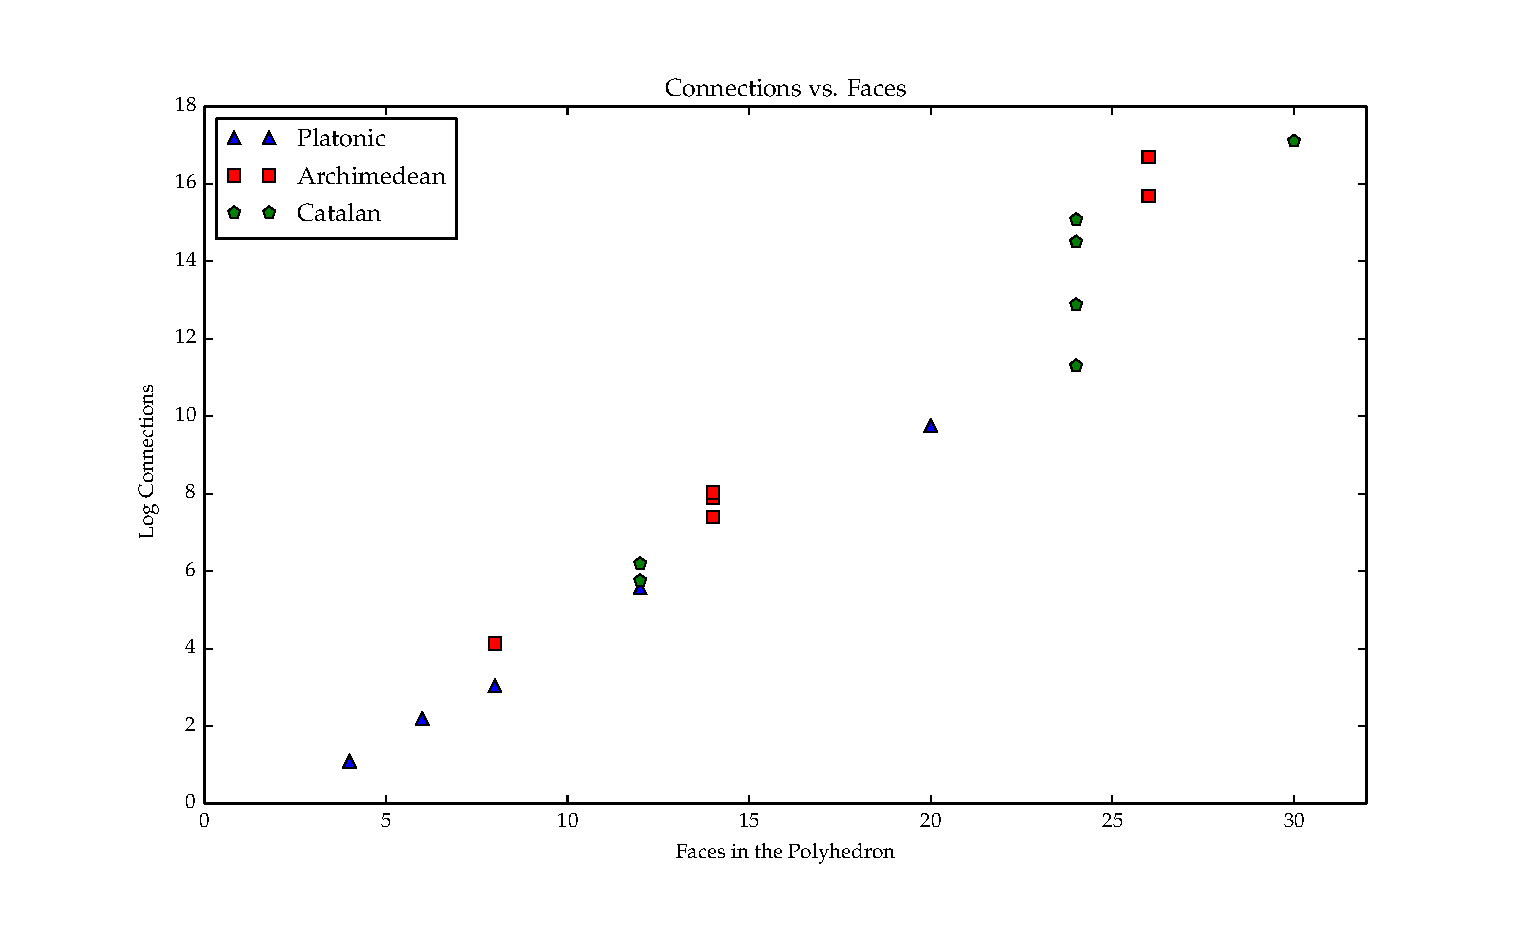
\includegraphics[scale=0.6, angle=0]{images/polys_face_con.eps}
\caption{The relation between number of faces and connections in the Building Game combinatorial configuration space.}
\label{fig:FacCon}
\end{figure}

\begin{figure}[ht]
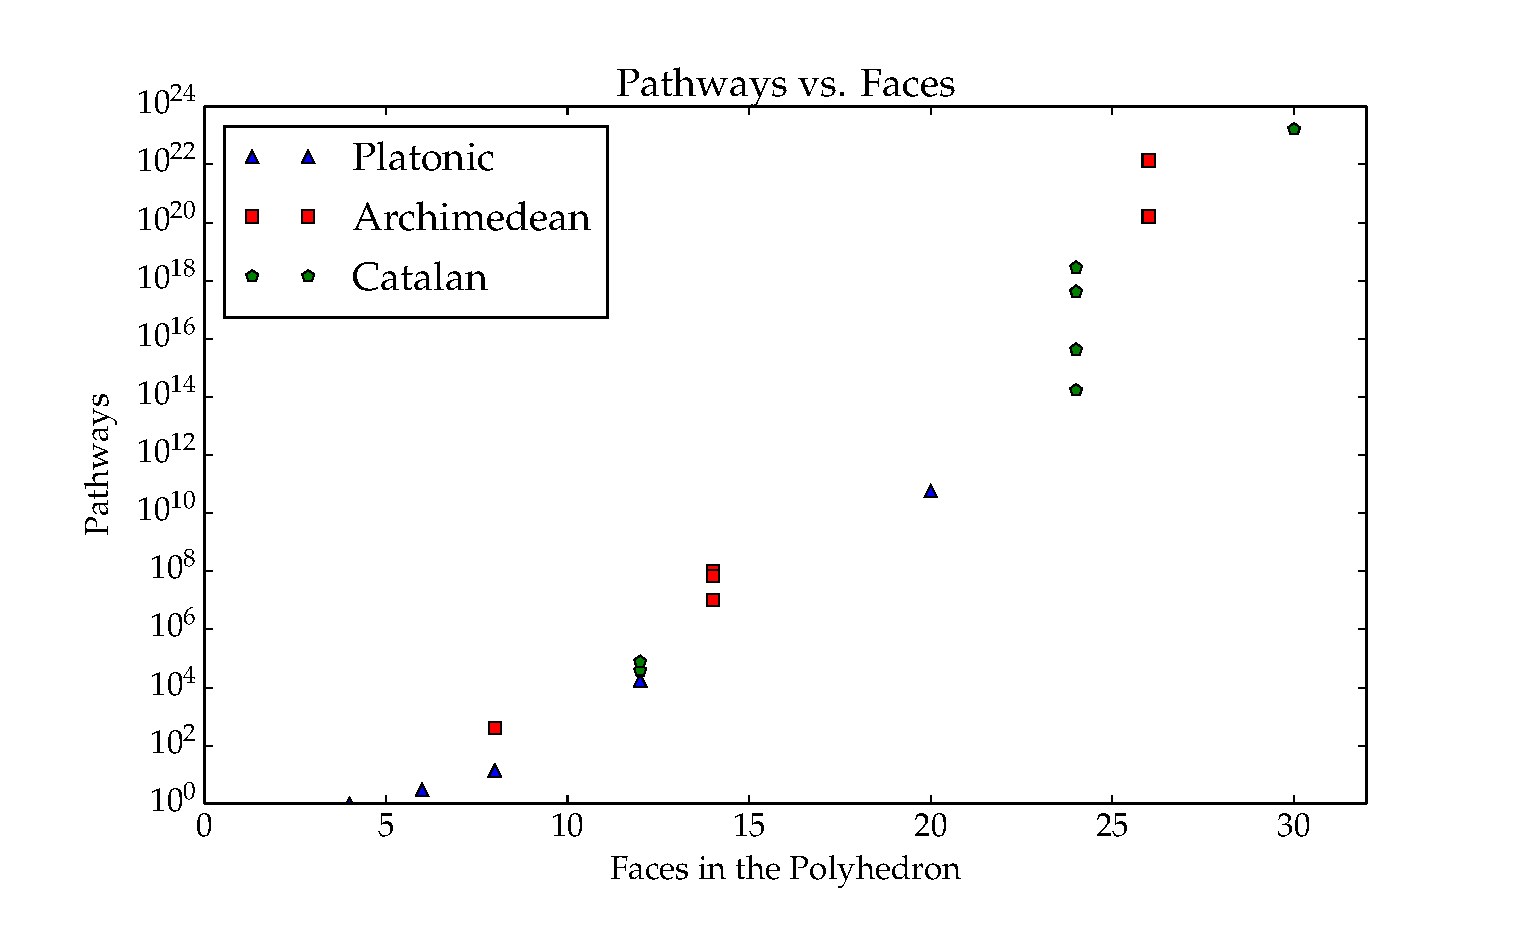
\includegraphics[scale=0.6, angle=0]{images/polys_face_path.eps}
\caption{The relation between number of faces and paths in the Building Game combinatorial configuration space.}
\label{fig:FacPath}
\end{figure}

\begin{figure}[ht]
\centering
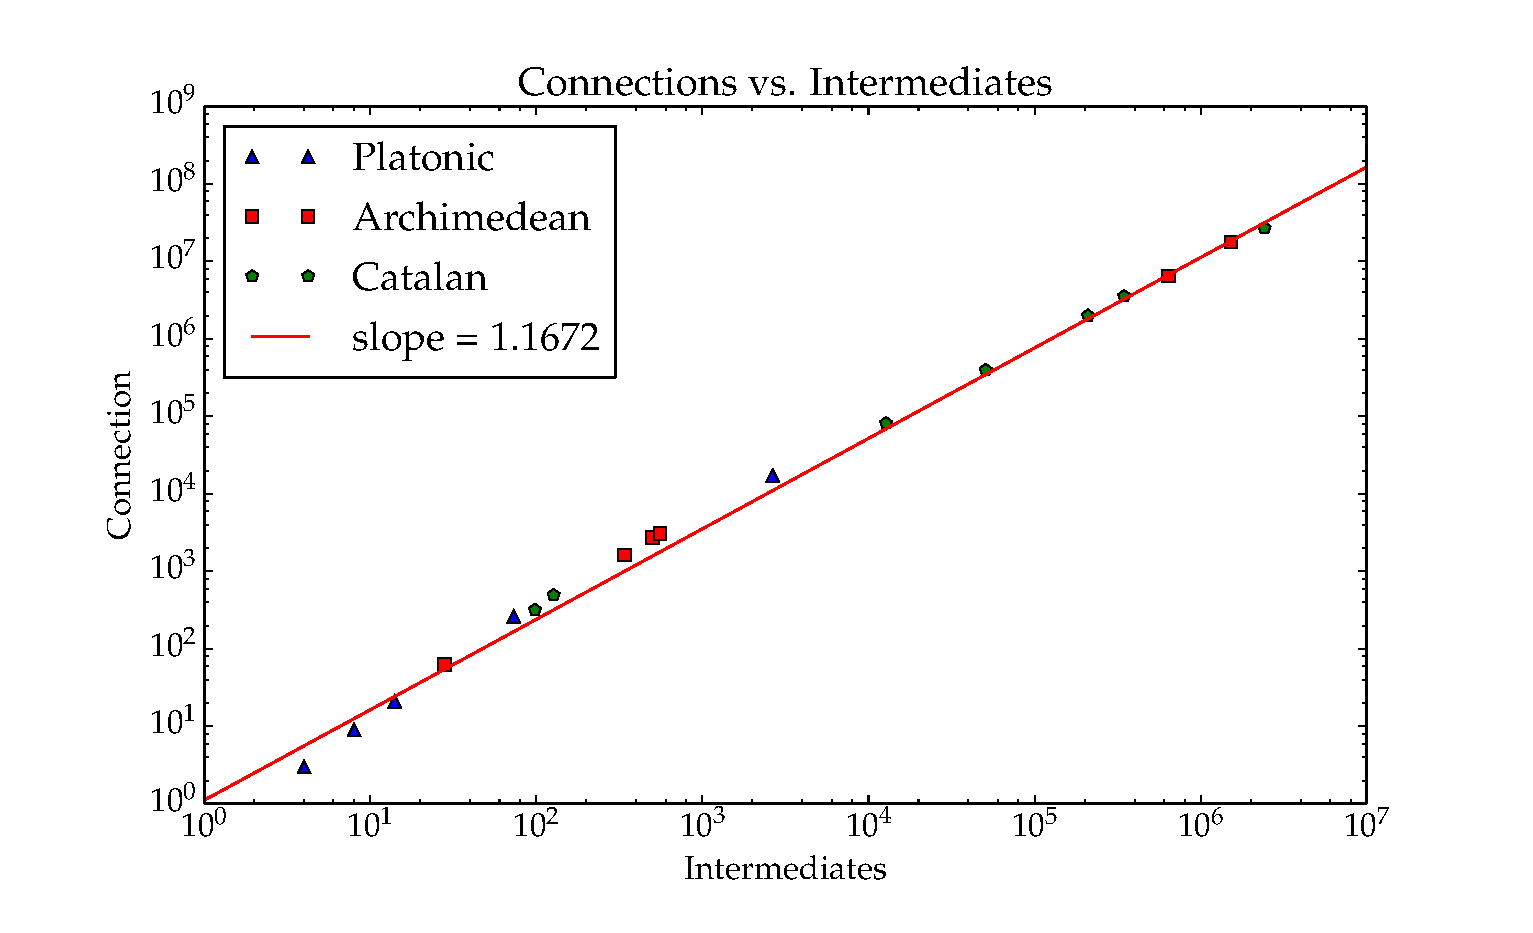
\includegraphics[scale=0.6, angle=0]{images/polys_int_con.eps}
\caption{The relation between number of intermediates and the number of connections in polyhedra.}
\label{fig:IntCons}
\end{figure}

\begin{figure}[ht]
\centering
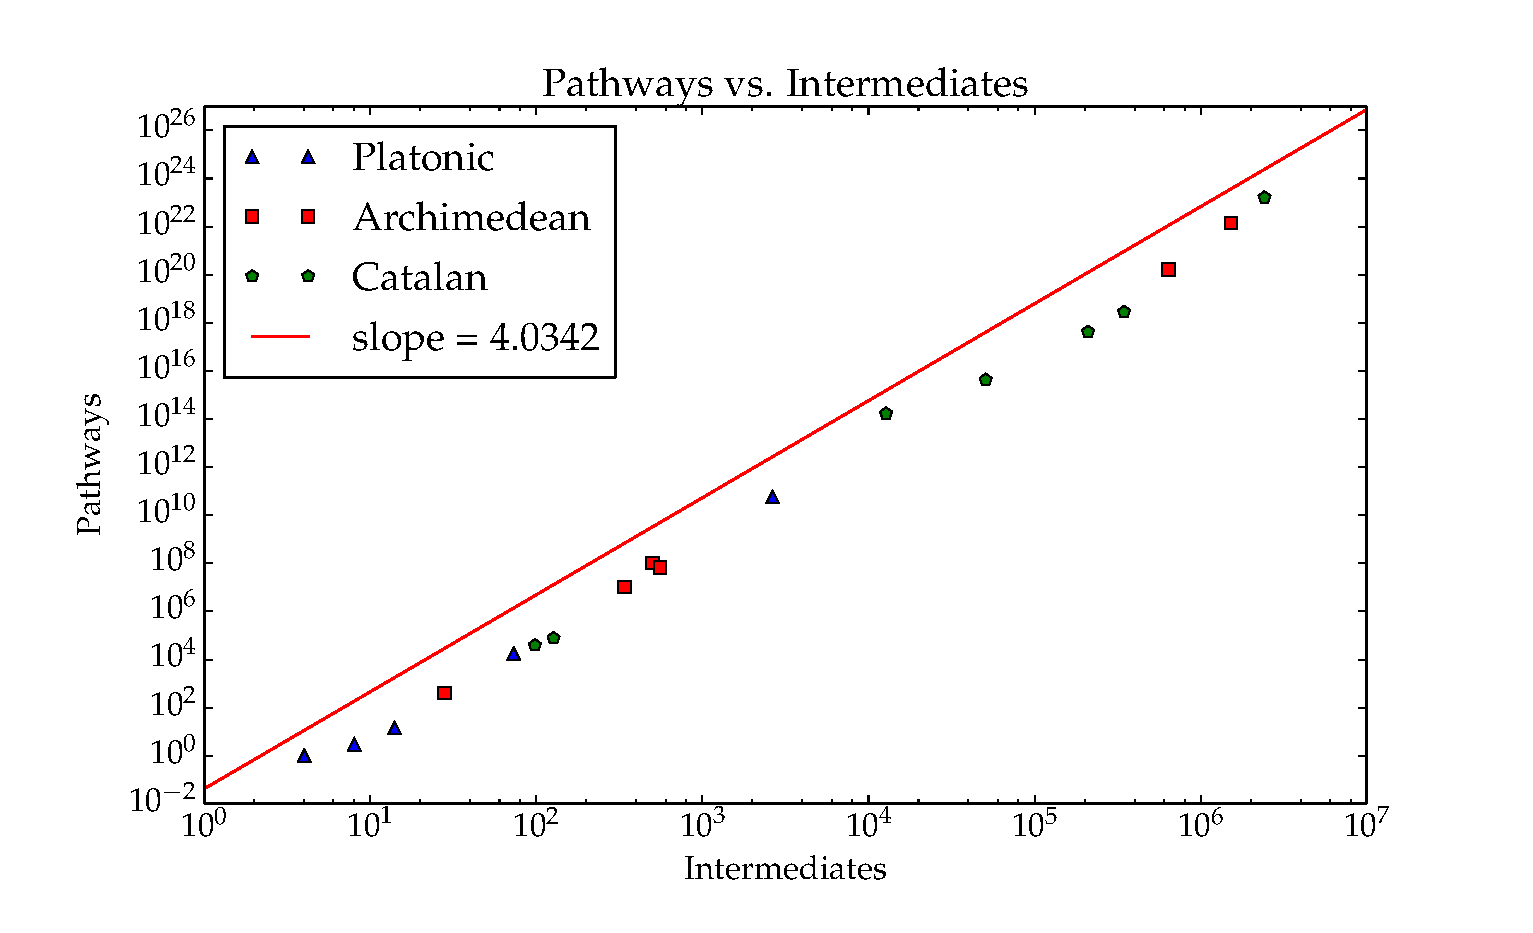
\includegraphics[scale=0.6, angle=0]{images/polys_int_path.eps}
\caption{The relation between number of intermediates and the number of pathways in polyhedra.}
\label{fig:IntPath}
\end{figure}

\begin{figure}[ht]
\centering
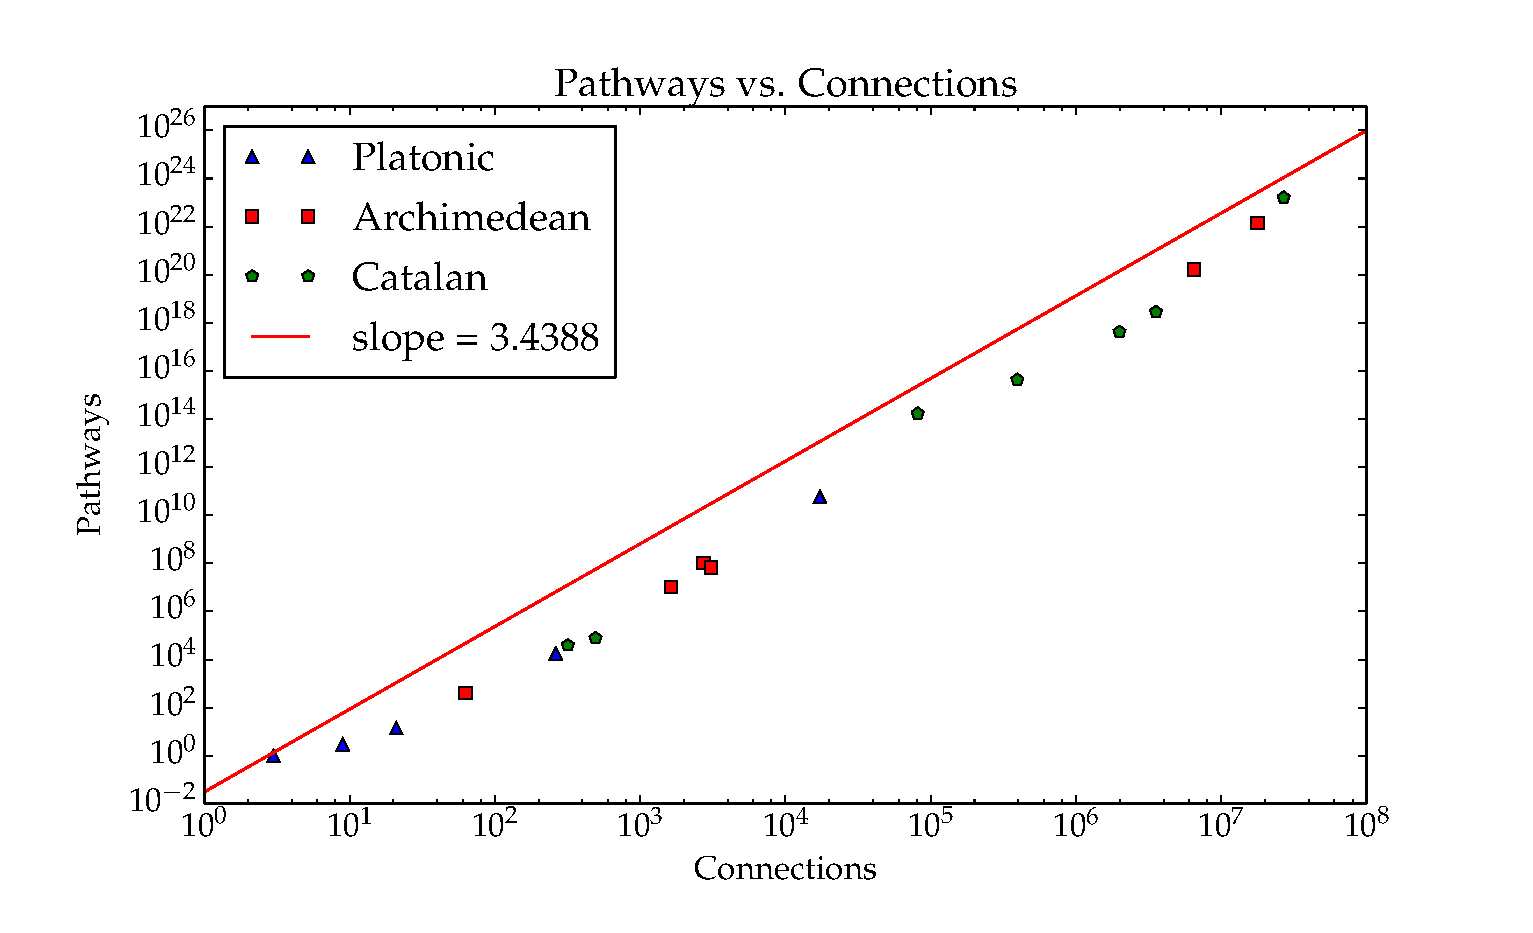
\includegraphics[scale=0.6, angle=0]{images/polys_con_path.eps}
\caption{The relation between number of connections and the number of pathways in polyhedra.}
\label{fig:ConPath}
\end{figure}



\subsection{Shellability}
The theory of polytopes provides a mathematical method for constructing a polytope called a \textit{shelling}. The process, similar to the building game, involves sequentially adding facets of the polytope until all of the facets are added. However, the rules as to which facets may be added at each step of the process are a bit more restrictive. Ziegler provides the following definitions of a shelling and a shellable polytopal complex~\cite{Ziegler1995}. 
\begin{mydef}
\label{def:shelling}
Let $\mathcal{C}$ be a pure $k$-dimensional polytopal complex $\mathcal{C}$. A \textbf{shelling} of $\mathcal{C}$ is a linear ordering $F_1,F_2,\dots,F_s$ of the facets of $\mathcal{C}$ such that either $\mathcal{C}$ is $0$-dimensional (and thus the facets are points), or it satisfies the following conditions:
\begin{enumerate}[(i)]
\item The boundary complex of the first facet $F_1$ has a shelling.
\item For $1 < j \leq s$ the intersection of the facet $F_j$ with the previous facets is non empty and is a beginning segment of a shelling of the $(k-1)$-dimensional boundary complex of $F_j$, that is,
$$F_j \cap \left(\bigcup_{i=1}^{j-1}F_i\right) = G_1 \cup G_2 \cup \cdots \cup G_r$$
for some shelling $G_1, G_2, \dots, G_r, \dots, G_t$ of $\mathcal{C}(\partial F_j)$, and $1 \leq r \leq t$. (In particular, this requires that $F_j \cap (\bigcup_{i=1}^{j-1} F_i)$ has a shelling, so it has to be a pure $(k-1)$-dimensional, and connected for $k > 1$.)
\end{enumerate} 
\end{mydef}

\begin{mydef}
A polytopal complex is \textbf{shellable} if it is pure and has a shelling. 
\end{mydef}

Since we are only concerned with $3$-dimensional polyhedra, the corresponding polytopal complex simply consists of the faces, edges, and vertices of the polyhedron. The facets of the complex are just the faces.

%\begin{mylem}
%The polytopal complex consisting of the verticies of a edge complex is shellable.
%\end{mylem}
%\begin{proof}
%\end{proof}


\begin{mydef}
A Building Game intermediate $x$ is called a \textbf{shellable intermediate} if for every state $x \in [x]$ there is a linear ordering $f_1, f_2, \dots, f_{|x|}$ on the faces of $x$ such that this ordering is a beginning of a shelling $f_1, f_2, \dots, f_{|x|}, \dots f_{|F|}$ of the polytopal complex $F\cup E\cup V$.
\end{mydef}

\begin{mylem}
The polytopal complex consisting of the edges and vertices of a polygonal face is shellable.
\end{mylem}
\begin{proof}
We see that condition $(i)$ from definition~\ref{def:shelling} is satisfied since the boundary complex of each edge is $0$-dimensional.

Condition $(ii)$ is also satisfied since each newly attached edge and the existing partial shelling is a subset of the attached edge's vertices. Since the vertices of the attached edge are $0$-dimensional, any linear order of its vertices is a shelling.
\end{proof}


%\begin{mythm}
%The poly  
%\end{mythm}

\begin{mydef}
A Building Game connection is said to be a \textbf{shellable connection} if the two connected intermediates are both shellable and a Building Game pathway is said to be a \textbf{shellable pathway} if each of its intermediates are shellable.
\end{mydef}

Figure~\ref{tab:bgEnumShell} details the shellability statistic for the Platonic, Archimedean, and Catalan solids classes. Because of the added shellability restriction, these count statistics are lower than in the general case, but the combinatorial growth as the number of faces increases is similar.  

%\begin{mylem}
%A shelling order cannot be fixed by a polyhedral rotation. 
%\end{mylem}
%\begin{proof}
%\end{proof}

\begin{figure}[ht]
\scalebox{0.85}{
\centering
%\textbf{Building Game Enumerative Results for the Platonic Solids}
\begin{tabular}{ l | c | r | r | r}
Polyhedra Name & $|F|$ & Intermediates & Connections & Pathways \\
  \hline    
Tetrahedron                     & 4     & 4     	& 5 		& 1\\
Cube                            & 6     & 7     	& 7 		& 2\\
Octahedron                      & 8     & 11    	& 13 		& 4 \\
Dodecahedron                    & 12    & 52    	& 155 		& 2,166\\
Icosahedron                     & 20    & 469   	& 1,985 	& 105,999,738\\  \hline    
Truncated Tetrahedron           & 8     & 21		& 40 		& 174\\
Cuboctahedron                   & 14	& 136		& 468 		& 477,776\\
Truncated Cube                  & 14	& 247		& 1,000 	& 5,232,294\\
Truncated Octahedron            & 14	& 342		& 1,464 	& 5,704,138\\
Rhombicuboctahedron             & 26	& 70,887	& 462,721 	& 64,308,526,503,247,584\\
Truncated Cuboctahedron         & 26	& 515,335	& 4,070,813	& 13,890,723,216,176,694,816\\  \hline    
Triakis Tetrahedron             & 12    & 48		& 115 		& 5,012\\
Rhombic Dodecahedron            & 12 	& 67		& 195 		& 6,258\\
Triakis Octahedron              & 24	& 1,021		& 4,237 	& 210,459,770,300\\
Tetrakis Hexahedron             & 24	& 4,224		& 21,125 	& 5,894,431,702,846\\
Deltoidal Icositetrahedron      & 24	& 33,046	& 208,317 	& 703,619,122,996,096\\
Pentagonal Icositetrahedron     & 24	& 95,326	& 657,013 	& 7,572,459,719,248,765\\
Rhombic Triacontahedron         & 30	& 97,741	& 702,219 	& 7,057,239,571,753,327,764\\
\end{tabular}
}
\caption{Building game enumerative shellability results for the Platonic, Archimedean, and Catalan solids.}
\label{tab:bgEnumShell}
\end{figure}

\begin{figure}[ht]
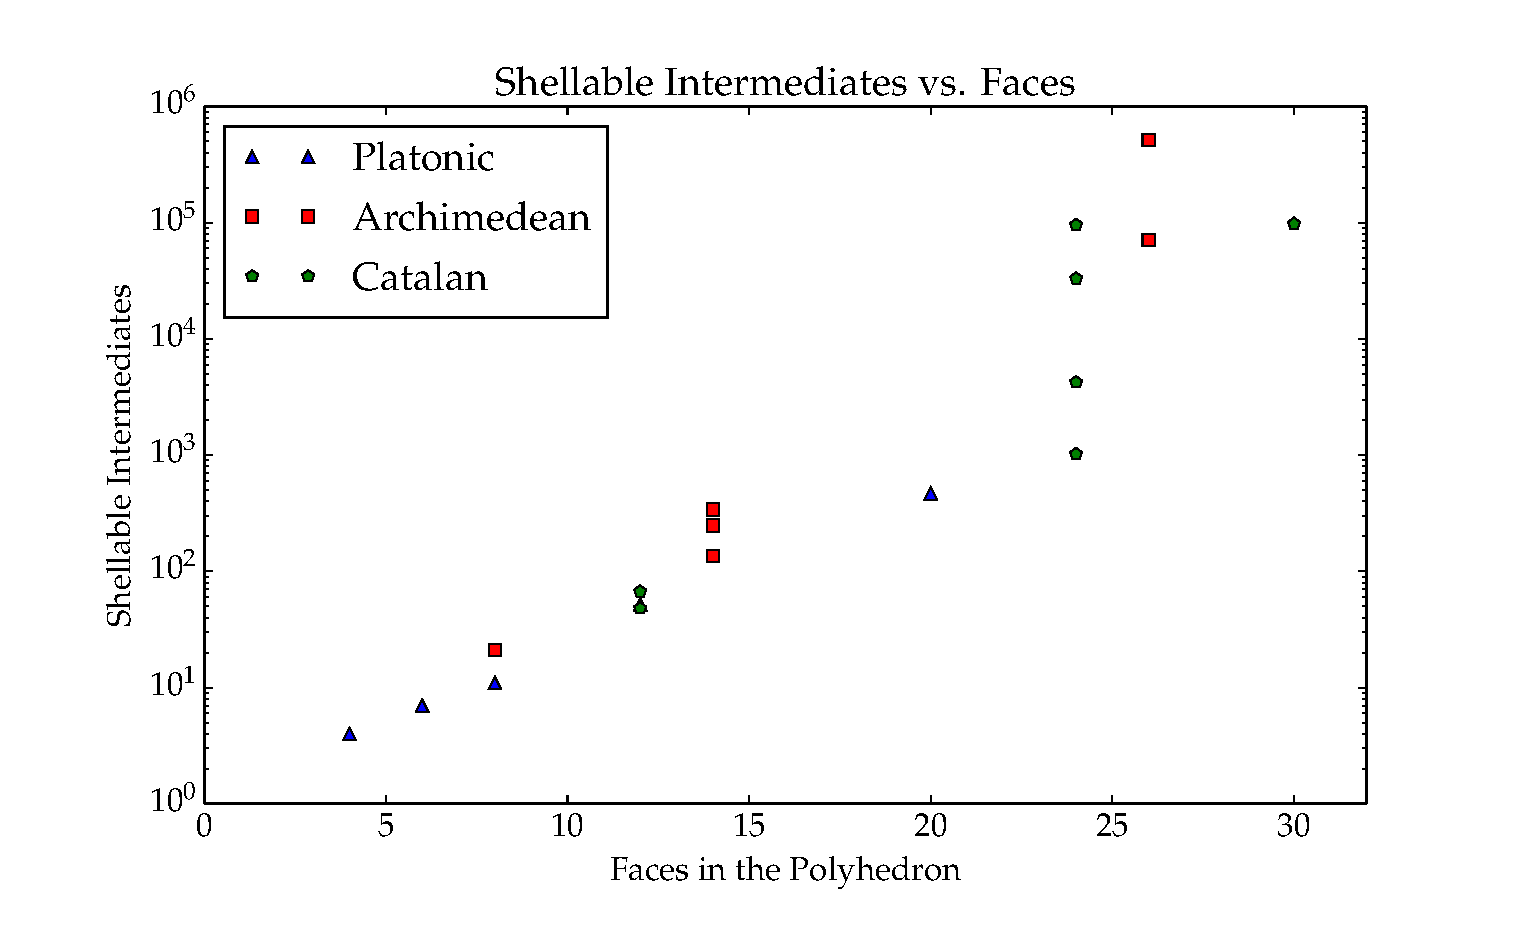
\includegraphics[scale=0.6, angle=0]{images/polys_face_shell_int.eps}
\caption{The relation between number of faces and shellable intermediates in the Building Game combinatorial configuration space.}
\label{fig:FacIntShell}
\end{figure}

\begin{figure}[ht]
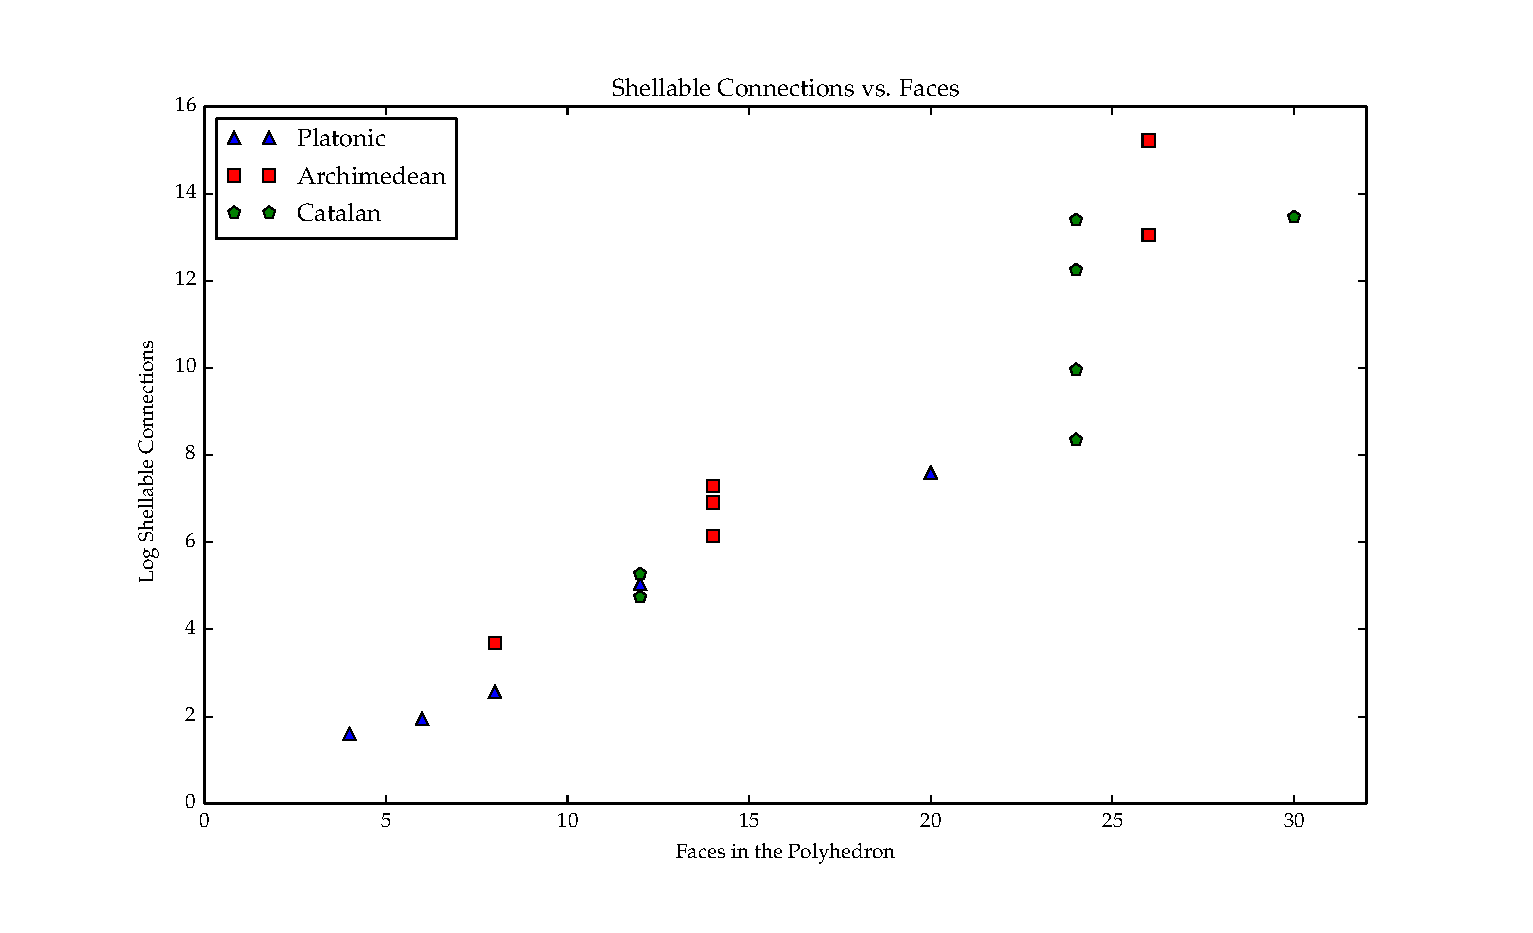
\includegraphics[scale=0.6, angle=0]{images/polys_face_shell_con.eps}
\caption{The relation between number of faces and shellable connections in the Building Game combinatorial configuration space.}
\label{fig:FacConShell}
\end{figure}

\begin{figure}[ht]
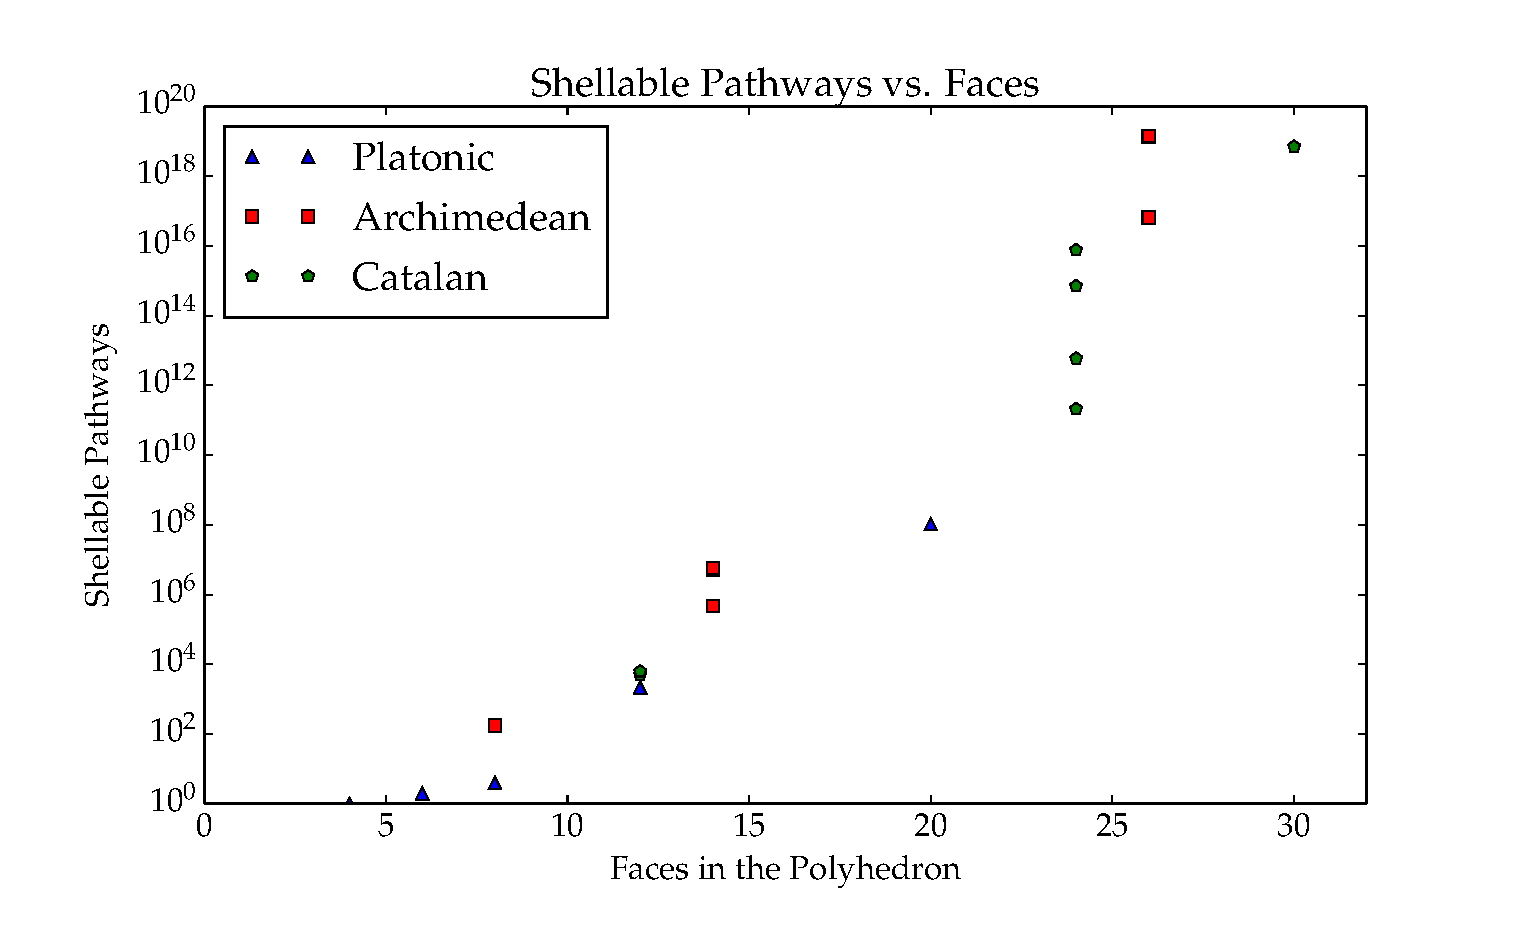
\includegraphics[scale=0.6, angle=0]{images/polys_face_shell_path.eps}
\caption{The relation between number of faces and shellable paths in the Building Game combinatorial configuration space.}
\label{fig:FacPathShell}
\end{figure}

\subsection{Shelling Enumeration}

To our knowledge, the enumeration of the number of shellings of the polyhedra in the Platonic, Archimedean, and Catalan solid classes remains an open problem. Here we present these enumerations for the polyhedra of up to $30$ faces. The concept of a shelling is similar to to that of a pathway. Using the structure of each computed combinatorial configuration space, a method for counting the number of shellings of a polyhedron is derived. 

\begin{mythm}
The total number of shellings for a polyhedral complex generated by a polyhedron is  
\begin{align}
\#(shellings) &= \sum_{p \in \{shell paths\}}|[x^{p_1}]|\prod_j^{|F|-1}S_{p_jp_{(j+1)}} .
\end{align}
\end{mythm}
\begin{proof}
We use the function that returns whether adding $f_k$ to the existing subshelling $f_1,\dots,f_{k-1}$ is itself a subshelling and call it $sh(\{f_1,\dots,f_{k-1}\}, f_k)$. Further, a Building Game connection between two shellable intermediates is called shellable and denoted  $[x^{p_i}] \xrightarrow{shell} [x^{p_{i+1}}]$. A pathway composed only of shellable intermediates and connections is called a $shellpath$. Using this notation, we compute the result directly.
\begin{align}
\#(shellings) &= \sum_{f_1 \in F} \mathbbm{1}_{sh(\emptyset,f_1)} \cdots\sum_{f_k \in F\setminus \{f_1,\dots,f_{k-1}\}} \mathbbm{1}_{sh(\{f_1,\dots,f_{k-1}\}, f_k)}\cdots \sum_{f_{|F|} \in F\setminus \{f_1, f_2, \dots, f_{|F|-1}\}}\mathbbm{1}_{sh(\{f_1, f_2, \dots, f_{|F|-1}\},f_{|F|})}  \\
&= \sum_{f_1 \in F} \mathbbm{1}_{sh(\emptyset,f_1)} \cdots\sum_{f_k \in F\setminus \{f_1,\dots,f_{k-1}\}} \mathbbm{1}_{sh(\{f_1,\dots,f_{k-1}\}, f_k)}\cdots \sum_{x^{p_{|F|}}: [x^{p_{|F|-1}}] \xrightarrow{shell} [x^{p_{|F|}}]} S_{p_{|F|-1}p_{|F|}}  \\
&= \sum_{f_1 \in F} \sum_{x^{p_2}: [x^{p_1}] \xrightarrow{shell} [x^{p_2}]} S_{p_{1}p_{2}}  \cdots \sum_{x^{p_{|F|}}: [x^{p_{|F|-1}}] \xrightarrow{shell} [x^{p_{|F|}}]} S_{p_{|F|-1}p_{|F|}}  \\
&= \sum_{[x^{p_1}} |[x^{p_1}]| \sum_{x^{p_2}: [x^{p_1}] \xrightarrow{shell} [x^{p_2}]} S_{p_{1}p_{2}}  \cdots \sum_{x^{p_{|F|}}: [x^{p_{|F|-1}}] \xrightarrow{shell} [x^{p_{|F|}}]} S_{p_{|F|-1}p_{|F|}}  \\
&= \sum_{p \in \{shell paths\}}|[x^{p_1}]|\prod_j^{|F|-1}S_{p_jp_{(j+1)}} 
\end{align}
\end{proof}

Using dynamic programming we can compute the number of shellings explicitly without having to explicitly consider each pathway individually. Define the quantity $a_{ik}$ as
\begin{align}
a_{i,k} &\doteq  \sum_{\substack{\text{shellable subpaths}:\\ p_1, \dots, p_k \\ x^{p_k} \in [x^i]}}|G.x^{p_1}|\prod_{j=1}^{k-1}S_{p_j p_{j+1}} \end{align}
where a subpath is the first $k$ intermediates in some valid pathway. Using this definition, we first note that the number of shellings, which is the quantity of interest, is equal to $a_{N,|F|}$ where $x^N = F$. Now, we set up the following recursion that will be the basis for our computation. 
\begin{align}
a_{i,k} &\doteq \sum_{\substack{\text{shellable subpaths}:\\ p_1, \dots, p_k \\ x^{p_k} \in [x^i]}}|G.x^{p_1}|\prod_{j=1}^{k-1}S_{p_j p_{j+1}} \\  
&= \sum_{[x^\ell]:[x^\ell]\xrightarrow{shell}[x^i]} \sum_{\substack{\text{shellable subpaths}:\\ p_1, \dots, p_{k-1} \\ x^{p_{k-1}} \in [x^\ell]}}|G.x^{p_1}|S_{\ell i}\prod_{j=1}^{k-2}S_{p_j p_{j+1}} \\
&= \sum_{[x^\ell]:[x^\ell]\xrightarrow{shell}[x^i]} S_{\ell i} \sum_{\substack{\text{shellable subpaths}:\\ p_1, \dots, p_{k-1} \\ x^{p_{k-1}} \in [x^\ell]}}|G.x^{p_1}|\prod_{j=1}^{k-2}S_{p_j p_{j+1}} \\
&= \sum_{[x^\ell]:[x^\ell]\xrightarrow{shell}[x^i]} S_{\ell i} a_{\ell, k-1}
\end{align}
Thus, using the base cases $a_{j,1} = |G.x^j|$ for each single faced intermediate $[x^j]$, we can use this relation to recursively solve for the number of shellings $a_{N,|F|}$.

\begin{figure}[ht]
%\scalebox{0.6}{
%{\footnotesize
\centering
%\textbf{Building Game Enumerative Results for the Platonic Solids}
\begin{tabular}{ l | c | r}
Polyhedra Name & $|F|$ & Shellings \\
  \hline    
Tetrahedron                     & 4  	& 24 \\                         
Cube                            & 6  	& 480 \\                        
Octahedron                      & 8  	& 4,224\\                       
Dodecahedron                    & 12 	& 19,041,600 \\                 
Icosahedron                     & 20 	& 1,417,229,099,520 \\ \hline   
Truncated Tetrahedron           & 8     & 9,216 \\                      
Cuboctahedron                   & 14	& 113,055,744 \\                
Truncated Cube                  & 14	& 654,801,408 \\                
Truncated Octahedron            & 14	& 937,087,104 \\                
Rhombicuboctahedron             & 26	& 4,728,400,467,971,102,208 \\  
Truncated Cuboctahedron         & 26	& 688,499,026,944,479,645,952 \\ \hline
Triakis Tetrahedron             & 12    & 587,040\\                     
Rhombic Dodecahedron            & 12 	& 5,836,800\\                   
Triakis Octahedron              & 24	& 66,063,419,534,592 \\         
Tetrakis Hexahedron             & 24	& 1,389,323,257,015,296 \\      
Deltoidal Icositetrahedron      & 24	& 125,987,819,253,281,472\\     
Pentagonal Icositetrahedron     & 24	& 1,144,572,832,023,047,616 \\  
Rhombic Triacontahedron         & 30	& 15,574,782,555,813,226,074,240 \\
\end{tabular}
%}
\caption{Number of Shellings for the Platonic, Archimedean, and Catalan solids of up to 30 faces.}
\label{tab:Shellings}
\end{figure}


\begin{figure}[ht]
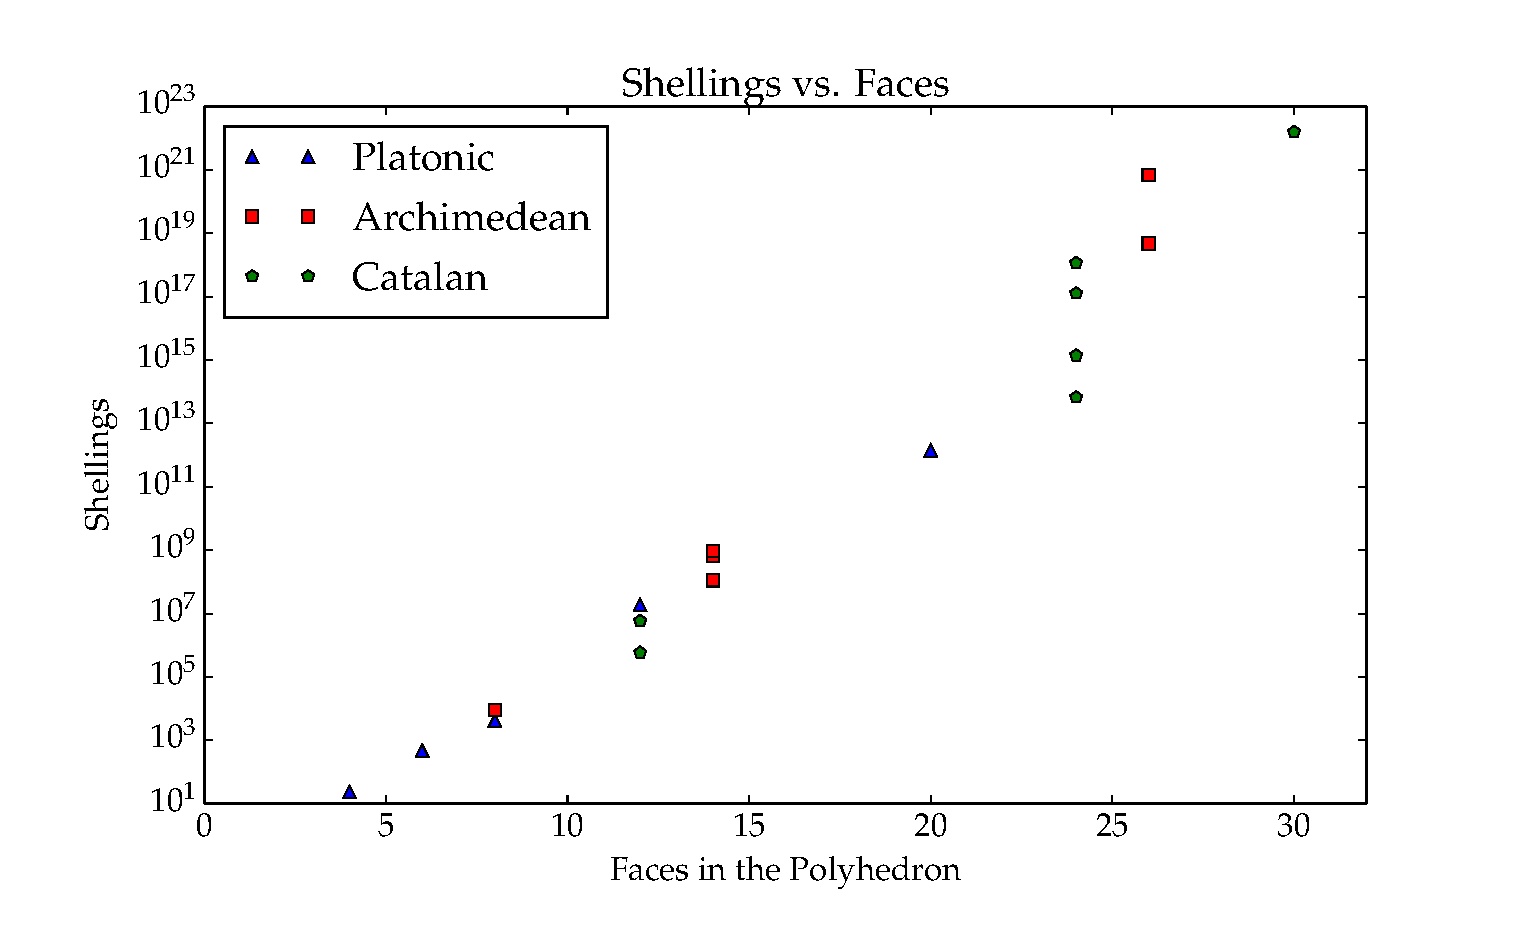
\includegraphics[scale=0.6, angle=0]{images/polys_face_shellings.eps}
\caption{The relation between number of faces and the number of shellings a polyhedron has.}
\label{fig:FacPathShellings}
\end{figure}

\subsection{Bounds and Asymptotics}
There is a clear relation between the number of faces in a polyhedron and then number of intermediates it has. However, that relationship also greatly depends on the polyhedral symmetry group. For instance, if you have a polyhedron with a small number of faces and a trivial rotation group consisting only of the identity, every edge-connected subset of the polyhedron's faces will be a distinct intermediate. In aggregate, this may mean that the polyhedron has more intermediates than another polyhedron with more faces, yet a larger symmetry group. 

An upper bound on the number of intermediates is possible using the theory of group actions. Consider the set of all subsets $2^F$ of a polyhedron with rotation group $G$. Trivially $|2^F/G|$ is an upper bound on the number of intermediates since it simply relaxes the connectivity requirement for a subset to be a building game state. Using Burnside's lemma, we see that 
\begin{align}
  \label{eq:IntUB}
  |2^F/G| &= \frac{1}{|G|}\sum_{g \in G}|(2^F)^g| \\
  &> \frac{|(2^F)^e|}{|G|} \\
  &= \frac{|2^F|}{|G|} \\
  &= \frac{2^{|F|}}{|G|}
\end{align}
which is not a particularly good bound in practice. The precise value of $|2^F/G|$ is calculable with minimal computer assistance, but details of this computation are omitted due to its relative uselessness. For the cube, the bound is fairly tight, only including the two non-intermediates corresponding to the empty subset of faces, and the non-connected subset consisting of the top and bottom faces. Thus the cube has the bound $|2^F/G| = 10 \geq 8$. In the case of the tetrahedron, the only over-counted subset of faces is the empty one and the bound is $|2^F/G| = 5 \geq 4$. However, in the case of the icosahedron we have $|2^F/G| \geq \frac{2^{20}}{60} \approx 17476.3 \gg 2649$. Here we use the approximate bound $\frac{2^{|F|}}{|G|}$ which is the largely dominant term in the sum from equation~\ref{eq:IntUB}.

We can get a similar bound on the number of intermediates with a particular number of faces,
\begin{align}
  |\{x \in 2^F: |x| = k\} /G| &= \frac{1}{|G|}\sum_{g \in G}|\{x \in 2^F: |x| = k\}^g| \\
  &> \frac{|\{x \in 2^F: |x| = k\}^e|}{|G|} \\
  &= \frac{|\{x \in 2^F: |x| = k\}|}{|G|} \\
  &= \frac{{|F| \choose k}}{|G|}
\end{align}
but again, this is not particularly useful, especially for intermediates with around $\frac{1}{2}|F|$ faces.

Since the building game is similar in spirit to polyomino enumeration, one might try to assimilate some the techniques used for polyominoes. For example, through fairly simple arguments, one can show that $s_ms_n \leq s_{m+n}$ where $s_m$ is the number of unique polyominoes with $m$ subunits~\cite{Klarner1973}. This leads to the bound $s_m \leq (const)^m$. Trying to set up such a relation in the building game is sounds initially appealing, but there is a fundamental difference between the two growth models that makes this approach futile. In the polyomino case, there is no limit to the number of subunits that can be considered. Importantly, this is not the case for the building game since an intermediate can only have $|F|$ faces at most. Thus any such recurrence relation for the building game will result in a good upper bound for the intermediates with a small number of faces at best.

The formulation of meaningful bounds for the number of building game intermediates with $k$ faces remains an open problem, especially for $k \sim \frac{1}{2}|F|$. At the root of the problem is the difficulty in mathematically describing the subsets of $F$ are edge connected. Future approaches may incorporate enumeration results for connected subgraphs or Hamiltonian paths since these topics explicitly acknowledge connectedness properties. 

From looking at the statistics on number of faces $|F|$ of a polyhedron and the number of intermediates in its combinatorial configuration space, it is natural to want to make statements about the asymptotic growth of the combinatorial configuration space's size. Unfortunately, when formed in this way, the problem is ill-posed. To discuss asymptotics, we must first specify an infinite class of polyhedra. The Platonic, Archimedean, and Catalan Solid classes that we've worked with thus far are all finite though, so other choices must be considered. One option is to take an existing polyhedron in one of these classes and create an infinite family by describing finer and finer tilings on top of the polyhedron's faces. If designed carefully each member of the tiled polyhedron family will have the same symmetry group, even as the number of faces grows. 

Similar to polyhedra with tiled faces are the icosahedral viral capsids indexed by T-number. This number is related to the number of protein subunits in the virus. When each subunit is idealized as a polygon, a T-capsid will consist of $12$ pentagons and $10(T-1)$ hexagons. Interestingly, this makes most of the icosahedral viral capsid equivalent to the dual of an icosahedron with each face consisting of $T$ triangular tiles. This would certainly be an interesting an relevant family of polyhedra to consider, though we leave it as an open problem.

\section{Computational Methods}

To compute the combinatorial configuration space and enumerate the intermediates for a particular polyhedron, we use a brute force method. Computation begins with first enumerating the intermediates with a single face. This enumeration is then used to compute the intermediates with two faces. This process proceeds iteratively until all intermediates are accounted for. Figure~\ref{alg:CCS} outlines the detailed algorithm for this computation. 

At each stage of our algorithm, we know the set of intermediates that have $k$ faces, which we call $A_k$, and use this information to compute the set of faces with $k+1$ faces, $A_{k+1}$. Since all intermediates in $A_{k+1}$ must be formed by adding a single face to an intermediate from $A_k$, we take each intermediate $[x] \in A_k$ and try adding each face to $x$ that is allowable under the building game rules. This means we look at every face $f \in F$ and check if $f \not\in x$ and also that $x$ is edge connected to a face $\hat{f}$ that is in $x$. For every such faces $f$, we look at the new $(k+1)$-faced state $y \doteq x\cup \{f\}$. Since we know that $[y]$ is a building game intermediate, it must be represented in $A_{k+1}$, however before adding $y$ to $A_{k+1}$, we must verify that there is no $\hat{y}$ already in $A_{k+1}$ such that $y \in [\hat{y}]$.

\begin{figure}[ht]
\centering
\begin{algorithmic}
  \State $A_1\gets \{\{f\} : f \in F\}$ 
  \For{$\{f\} \in A_1$}
  \If{$\exists \{\hat{f}\} \in A_1 \setminus \{f\} : [\{\hat{f}\}\ ]= [\{f\}]$}
  \State $A_1 \gets A_1 \setminus \{\{f\}\}$
  \EndIf
  \EndFor
  \State $A_2, \dots, A_{|F|} \gets \{\}$ 
  \For{$k = 0,\dots,|F|-1$}
  \For{$x \in A_k$ }
  \For{$f \in F\setminus x$ such that $\exists \hat{f} \in x$ with $f$ and $\hat{f}$ sharing an edge. }
  \State NewIntermediate $\gets True$
  \For{$\hat{y} \in A_{k+1}$}
  \If{$y \in [\hat{y}]$}
  \State NewIntermediate $\gets False$
  \State Add connection $[x] \leftrightarrow [\hat{y}]$ to combinatorial configuration space.
  \EndIf
  \EndFor
  \If{NewIntermediate $= True$}
  \State $A_{k+1} \gets A_{k+1} \cup \{y\}$
  \State Add connection $[x] \leftrightarrow [y]$ to combinatorial configuration space.
  \EndIf
  \EndFor
  \EndFor
  \EndFor
\end{algorithmic}
\caption{Algorithm for iteratively enumerating the Building Game combinatorial configuration space.}
\label{alg:CCS}
\end{figure}

The act of comparing two states $y$ and $\hat{y}$ to check if they are members of the same intermediate is the task where the majority of computational time is spent. The brute force method of checking if $y \sim \hat{y}$ involves checking if $g.y = \hat{y}$ for each $g \in G$. If a $g$ is found that makes this equality hold, then $[y] = [ \hat{y}]$ and the computation terminates and we know that $[y]$ is not a new intermediate. In this case, nothing is added to $A_{k+1}$ but a connection $x \leftrightarrow \hat{y}$ is added in the combinatorial configuration space. Furthermore, by tracking how many time a particular connection $x \leftrightarrow \hat{y}$ is found, the forward degeneracy numbers can be computed quickly. 

\subsection{Hash Functions}
In practice, we implement a hash function $\textswab{h}$ that maps each state to an integer with the property that if $[y] = [\hat{y}]$, then $\textswab{h}(y) = \textswab{h}(\hat{y})$. If we can design such a function and it is computable in significantly less time relative to the brute force method of trying every rotation, the overall computation can be majorly diminished. 

When checking if two states $y$ and $\hat{y}$ are members of the same intermediate, we first check if $\textswab{h}(y) = \textswab{h}(\hat{y})$. If they do not have the same hash, then they cannot be members of the same intermediate and the check is complete. Alternatively, if they do have identical hashes, it is not a guarantee that they are members of the same intermediate, so the brute force rotation method must be used. If the hash is carefully designed then this false positive rate ($\textswab{h}(y) = \textswab{h}(\hat{y})$ when $[y] \neq [\hat{y}]$) is small and almost all of the brute force calculations will result in a positive match. 

In an ideal world, a hash function that also gives the property $[x] = [\hat{x}]$ whenever $\textswab{h}(x) = \textswab{h}(\hat{x})$ would be best. However we have not been able to find such an $\textswab{h}$ that is computable in a relatively reduced amount of time in comparison to the brute force method. We leave the existence of such a hash as a possibility. 

Since any hash we choose must a function that maps states that are rotations of each other to the same integer, we look at local connectivity properties. For each face $f_k \in F$ define its local connectivity within $y$ as  $\textswab{h}_k(y) = |\{\hat{f} \in F : \hat{f} \in y, f_k \cap \hat{f} \in E\}|$, the number of faces adjacent to $f_k$ that are also in $y$. Since this connectivity is preserved by rotations, even though we wont necessarily have $\textswab{h}_k(y) = \textswab{h}_k(\hat{y})$ when $[y] = [\hat{y}]$, if we take a histogram of all values of $\textswab{h}_k$ for $k = 1,\dots,|F|$, the histogram will be the same for both $y$ and $\hat{y}$. Once a histogram is computed, the final hash $\textswab{h}$ is just a simple function that maps histograms to integers.

There are many variants of statistics that this histogram strategy can be used with. We found that taking separate histograms for faces in $y$ and faces not in $y$ provided a hash with less false positives, while only increasing the hash computation time marginally. Depending on the polyhedron, the implementation of this hash lead to an over all speed up of at least an order of magnitude over the purely brute force method.  

\subsection{Data Structures}

Before the computation of the combinatorial configuration space, we hard-code an enumeration $f_1, \dots, f_{|F|}$ of the faces of our polyhedron. Then, any state $x$ is represented by a binary vector of length $|F|$ with a one in the $k$th entry if $f_k \in x$ and zero otherwise. With this convention, each rotation $g \in G$ corresponds to a permutation of the indices of $x$. Each such permutation in the group is precomputed and then applied as necessary when performing a brute force comparison of two states. To track the connectivity structure of the polyhedron, an adjacency list on faces is stored as a two dimensional array. For each face number, the adjacency list specifies the index of adjacent faces.

Each group of $k$-faced intermediates $A_k$ is stored as a hash table using the previously described hash function. This allows for order one look-up of intermediates already in the $A_k$ that share the hash of a new proposal intermediate. 

\subsection{Run Time}

The computing time required to enumerate the combinatorial configuration space is heavily dependent on the number of intermediates that are found. Since we do not have a tight bound on the number of intermediates as a function of simple statistics of the polyhedron (faces, edges, etc.), it is difficult to provide a meaningful estimates on the time required to compute the combinatorial configuration space without explicit knowledge of its size a priori.

That said, we can express an upper bound on the number of state to state comparisons that are required as a function of the intermediate sets $A_1,\dots,A_{|F|}$. 

\begin{align}
\#\text{comparisons} &\leq \sum_{k=1}^{|F|-1} \sum_{x \in A_k} \sum_{f \in F\setminus x} \sum_{\hat{y} \in A_{k+1}} 1 \\
&\leq |F|\sum_{k=1}^{|F|-1}|A_k||A_{k+1}| 
%&\leq |F|\sum_{k=1}^{|F|-1} {|F| \choose k} {|F| \choose k+1}  \\
\end{align}


\subsection{Implementation}
All computation was carried out on a desktop computer running 64-bit Ubuntu 14.04 LTS with 15.6 GiB memory and a quad-core 3.20GHz Intel processor. To compute the building game combinatorial configurations space, we developed C++ code with the help of the Boost graph library for storing the connectivity structure. Computation of the combinatorial configuration space took less than a minute for most polyhedra, though--as expected--this time grew dramatically with the number of faces. Our largest case, the 30-faced Rhombic Triacontahedron took on the order of 10 minutes to compute. 

Additional computation--especially for pathway and shelling statistics--was completed using Python and the mpmath module for arbitrary precision arithmetic~\cite{mpmath}. 

\clearpage{\pagestyle{empty}\cleardoublepage}

\chapter{Constraint Models and Embedding Intermediates in Space}

While models such as the Building Game treat assembly intermediates as idealized structures, the intermediates of the physical application we are modeling may face unpredictable forces. To realistically model the ways in which our intermediate might flex and move under these forces, we use a constraint model in which individual faces of an intermediate are rigid, but with the edges at which two faces meet modeled as a hinge. As seen in figure~\ref{fig:OctaGCS}, this approach allows for a variety of geometric configurations while the combinatorial connectivity properties of the intermediate remain unchanged.  This geometric framework provides a physically motivated way of addressing questions that strictly combinatorial models cannot adequately answer. 


\begin{figure}[ht]
       \centering
                
\includegraphics[width=0.3\textwidth]{images/OctaGCS_0.eps}
                
\includegraphics[width=0.3\textwidth]{images/OctaGCS_1.eps}
                
\includegraphics[width=0.3\textwidth]{images/OctaGCS_2.eps}

\caption{Different geometric configurations of an octahedron intermediate.}
\label{fig:OctaGCS}
\end{figure}


\begin{mydef}
The \textbf{canonical configuration} of a Building Game intermediate $[x]$ is the configuration that is the $3$-dimensional embedding of the polyhedron restricted to the faces in $x$
\end{mydef} 
 For example, in the case of the cube, the canonical configuration would have all of the faces of the intermediate meeting at right angles just as they do in the cube itself, however this is just one possible geometric configuration.




%\subsection{Configuration Space}

%To characterize the freedoms of three-dimensional intermediates composed of rigid two-dimensional faces and connected at hinged edges, we parameterize each face and impose constraints in parameter space. Theoretically, the location and orientation of each face of an intermediate can be parameterized by six parameters: three for translation, three for rotation. This means the configuration of the entire intermediate can be represented by at most $6|F|$ parameters. In practice, however, it is often advantageous for ease of analysis and computational implementation to use more parameters to represent a given configuration. Often times, we use $3$ parameters to represent the location each vertex of each face, even if some of these vertices share common locations. This means that we often have an ambient parameter space of $\mathbb{R}^N$ with $N > 6|F|$. 

%Upon this parameter space we place three types of constraints. The first removes the configuration's 6 trivial degrees of freedom due to translation and rotation. Since the intermediate is connected, this can be achieved by fixing the parameters of one of the intermediate's faces. Additionally, we enforce a rigidity constraint on each face ensuring that the structure of a constituent face will not change with movement of the larger structure. The final type of constraint ensures that the connections between two faces have hinge-like mobility. Since a shared edge has two vertices belonging to each face, this constraint is imposed by identifying the corresponding vertex locations. 

%The \textit{configuration space} is defined to be the subset of ambient space $\left\{z \in \mathbb{R}^N : \varphi\left(z\right) = 0\right\}$  for which all $M$ of the constraint equations $\varphi: \mathbb{R}^N \to  \mathbb{R}^M $ are satisfied.  Since it is assumed that the standard configuration of the intermediate given by the model satisfies the constraints, the configuration space is non-empty. The configuration space is an algebraic variety, because the constraint equations can typically be represented as (quadratic) polynomials.  The \textit{degrees of freedom} of a particular configuration is taken to be the dimension of the null space of the Jacobian of $\varphi$. This is due to the fact that any move in the ambient space that prevents the constraint equations from changing must also be in the configuration space. Interestingly, it is possible for some members of configuration space to have a different number of degrees of freedom than others. 
 
%It is important to note that there are many possible parameterizations of a configuration and the choice of which will likely result in a different configuration space. The selection of which face to constrain in order to remove the trivial degrees of freedom may also affect the structure of the configuration space. While we must be cognizant of these choices, in many cases, the properties we wish to evaluate of the configuration space are independent of the choices.

%\subsection{Cyclohexane}
%
%One example of using the 
%

%\section{Linkages and Frameworks}
%--izmestiev def of framework
%--freedom in machines def of linkage
%--used to describe configurations and freedoms 


\section{Geometric Configuration Space}
%
%\begin{mydef}
%The \textbf{constraint space} corresponding to a constraint function $c: \mathbbm{R}^n \to \mathbbm{R}^{n-m}$ is its zero-set,
%\begin{align}
%\Omega \doteq \{z \in \mathbbm{R}^n : c(z) = 0\}.
%\end{align}
%\end{mydef}



Using a system of constraint functions, we can mathematically define the space of different geometric configurations that a given intermediate can take. Since we are treating each intermediate as collection of rigid polygons attached to each other along hinged edges, there are two basic types of constraint we must enforce. First, we must ensure that the each individual face is rigid and has the correct geometric shape. Additionally, each edge to edge connection must remain fixed with only hinge-like motion allowed. By defining this set of constraints as a single constraint function $c: \mathbbm{R}^n \to \mathbbm{R}^{n-m}$, the solution set $\Omega \doteq \{z \in \mathbbm{R}^n : c(z) = 0\}$ is the set of points where all of the constraints are simultaneously satisfied. This constraint system implicitly specifies all of the ways in which an intermediate has freedom to move if it is able to move at all. If $c$ is composed of polynomial functions, then the solution set is an algebraic variety. If this variety has no singularities, then it is also a manifold. 


\begin{mydef}
The \textbf{geometric configuration space} of a Building Game intermediate is an algebraic variety corresponding to a system of polynomial constraints that enforces the rigidity of individual faces and hinged motion along connected edges.
\end{mydef}



To mathematically describe a particular configuration, we must specify the locations of the vertices of each face. Thus, for an intermediate $[x]$, its Building Game configuration space can be represented as a subset of the ambient space $\mathbb{R}^{3\times N_x}$ where $N_x \doteq \sum_{f\in x} s_f$ where $s_f$ is the number of sides (and vertices) of face $f$. Using this representation, we must then identify the corresponding constraint equations that give rise to the combinatorial configuration space as a function of points in ambient space. 

It is worth noting that while we represent each face with $3\times s_f$ coordinates, only 6 are required to specify a face's position and orientation if they are chosen carefully. With this in mind, we will typically use a function of $6$ of a face's vertex coordinates to constrain each of the face's remaining vertex coordinates. 


Notationally, we refer to the $k$th vertex of the $j$th face of $x$ as $v^{jk} = \left(v^{jk}_x,v^{jk}_y,v^{jk}_z\right)$. Since the context of a solution variety requires a function $c: \mathbbm{R}^n \to \mathbbm{R}^{n-m}$, we flatten the matrix of vertex coordinates into a vector of length $n = 3N_x$. 
\begin{align}
z = \begin{bmatrix} v^{1,1} \\ \vdots \\ v^{1,s_{f_1}} \\ \vdots \\ v^{|x|,1} \\ \vdots \\ v^{|x|,s_{f_{|x|}}} \end{bmatrix} \in \mathbbm{R}^n
\end{align}

There are four fundamental types of constraint equations: edge length constraints, angle constraints, and $2D$ face constraint to enforce the rigid structure of each face as well as vertex identification constraints to enforce the hinged connections. The equations for these constraints are outlined in table~\ref{tab:cons} with an extended discussion appearing in section~\ref{ssc:cons}

\begin{table}
\label{tab:cons}
\begin{tabular}{ l | l}
Constraint Type & Constraint Equation \\
  \hline    
edge length & $c_{edge}^{j,k}\left(z\right) = \left|v^{j,k} - v^{j,k-1}\right|^2 - (\ell_{j,k})^2$ \\
angle & $c_{ang}^{j,k}\left(z\right) = (v^{j,k-1} - v^{j,k})\cdot(v^{j,k+1} - v^{j,k})  - \ell^{j,k}\ell^{j,k+1}\cos(\theta^{j,k})$\\
2D face & $c_{2D}^{j,k}(z) = v^{1,k} + \ell^{j,k,1}R(v^{j,0} - v^{j,1}) - v^{j,k} $\\
vertex identification & $c_{ident}^{j_1,k_1,j_1,k_1,d}(z) = v^{j_1,k_1}_d - v^{j_2,k_2}_d$ 
\end{tabular}
\caption{The different types of polynomial constraint equations used to describe the geometric configuration space.}
\label{tab:cons}
\end{table}


%To mathematically represent each of the possible geometric configurations, we parameterize the embedding using its vertex locations. If a Building Game state is composed of the faces $\{f_1,\dots, f_i\}$, then any embedding of the intermediate can be described by a point in $\mathbbm{R}^n$, where $n$ is the three times sum $3\sum_{j=1}^i \#\text{vertices}(f_j)$, of the number of vertices in each face. Simply put, the point 
% which is the concatenation of all of the vertex locations $v_1, v_2, \dots, v_{n/3} \in \mathbbm{R}^3$ for each verted on each face of an intermediate is used to represent a particular embedding. 

\subsection{Special Case of Triangular Faces}

In the case where all of the faces of the polyhedron we consider are triangles (tetrahedron, octahedron, icosahedron, etc.) we notice that by simple enforcing that each edge of each triangle has a specified length, the triangle will be rigid. This means that we do not have to use the angle and 2D face constraints. Further, rather than explicitly using vertex identification constraints, we can either treat them as length constraints with zero length between identified vertices or we can simply reindex the vertices so that identified vertices are actually treated as a single vertex. With either choice, in the triangular case, we may only deal with length constraints if we wish. This will be a useful property in the next chapter. 

%Additionally, we make a conjecture that under certain triangular conditions, our algebraic variety has no singularities and is thus a manifold.
%\begin{mycon}
%\label{con:TriMan}
%The geometric configuration space for each intermediate composed of equilateral triangular faces is a manifold.
%\end{mycon}

\section{Degrees of Freedom}
\label{ssc:cons} 
Roughly speaking, the degrees of freedom of a system are the different independent motions the system is able to exercise. Since the concept of degrees of freedom exists in many diverse scientific fields, such as mechanical engineering and statistical physics, many different formal definitions of degrees of freedom are used in the literature~\cite{Pennestri2005}. McCarthy defines degrees of freedom of a mechanical system as follows~\cite{McCarthy1990}. 
\begin{quote}
We derive formulas for the number of parameters needed to specify the configuration of a mechanism, in terms of the number of links and joints and the freedom of movement allowed at each joint. This number is the \textit{degrees of freedom} or \textit{mobility} of the mechanism. Changing the values of these parameters changes the configuration of the mechanism. Thus, if we view the set of all configuration available to a mechanism as a manifold, then the mobility of the mechanism is the dimension of this manifold. 
\end{quote}

Since our geometric configuration space is an algebraic variety and not a manifold in general, this definition must be modified to make degrees of freedom a statistic of each individual configuration rather than a global statistic of the geometric configuration space. 

\begin{mydef}
The number of \textbf{degrees of freedom} of a Building Game intermediate at configuration $z$ is the dimension of the geometric configuration space at $z$. If $z$ is a singularity of the algebraic variety, then the degrees of freedom is undefined.
\end{mydef}

In most cases we consider, rigid rotation and rigid translation will preserve the value of the constraint function since they do not move the vertices relative to one another. In other words, if $c(z) = 0$ then we also have $c(Rz + T) = 0$ where $R \in \mathbbm{R}^{n}\times n$ rotates each vertex in the configuration by some $\hat{R} \in SO(3)$ and translates each vertex by $\hat{T} \in \mathbbm{R}^3$. With this definition, $R$ is the block diagonal matrix with each of the $n/3$ block being $\hat{R} \in SO(3)$ and $T \in \mathbbm{R}^n$ is composed of $n/3$ copies of $\hat{T} \in \mathbbm{R}^3$ stacked upon each other. These rigid body rotations account for $6$ of the configuration's degrees of freedom: $3$ rotational degrees of freedom and $3$ translational and are called the \textit{trivial degrees of freedom}. Thus, the degrees of freedom we are most interested in are those that do represent movement of the vertices and faces relative to each other. The \textit{internal degrees of freedom} a Building Game intermediate at configuration $z$ are the degrees of freedom that are not trivial.


\subsection{Computing Degrees of Freedom}

For a generic solution variety, we can find the dimension of the space at a point $z$ by looking at the Jacobian matrix $C(z) \in \mathbbm{R}^{(n-m)\times n}$ of the constraint function $c$. Since the number of degrees of freedom is defined to be the dimension of that space, we look at the rank of the Jacobian. Since this rank quantifies the number of independent constraints given by $c$ at $z$, the number of degrees of freedom is given by the following.
\begin{align}
DoF &\doteq n - \text{rank}\left((C(z)\right)
\end{align}
Since the rank can take values between $0$ and $\min\{n,n-m\} = n-m$, there can be anywhere from $0$ degrees of freedom, when there are functionally no constraints on $z$, and $m$ degrees of freedom in the case where all $n-m$ constraint equations are independent and $C(z)$ is of full rank. 

In the typical case in which the constraint equations are invariant under three-dimensional rotation and translation, there will be six trivial degrees of freedom. The number of internal degrees of freedom would then be $n - \text{rank}\left((C(z)\right) - 6$. If there are zero internal degrees of freedom at a configuration $z$, we say that the configuration is \textit{rigid}.

To actually compute the number of degrees of freedom for configurations of Building Game intermediates, we must first find an explicit form for the the constraint function $c$ and its Jacobian matrix $C$.

Edge length constraints enforce that the lengths of the edges of each face in an intermediate cannot change. If the $k$th edge is defined to be that between the $(k-1)$st and $k$th vertices, we use the following function to constrain its lengths to a known value $\ell^{jk}$.
\begin{align}
c_{edge}^{j,k}\left(z\right)& = \left|v^{j,k} - v^{j,k-1}\right|^2 - (\ell_{j,k})^2 \\
& = \left(v_1^{j,k} - v_1^{j,k-1}\right)^2 +\left(v_2^{j,k} - v_2^{j,k-1}\right)^2 +\left(v_3^{j,k} - v_3^{j,k-1}\right)^2 - (\ell^{j,k})^2 
\end{align}  
This uses the notational convention that $v^{j,0} \doteq v^{j,s_j}$. For reasons that will be explained, we only explicitly enforce the lengths of two edges ($k=1,2$) per face, so there are a total of $2|x|$ edge length constraints. 

Angle constraints ensure that each face's polygonal angles are conserved. Using the dot product formula for angles, we can write this constraint as a polynomial.
\begin{align}
c_{ang}^{j,k}\left(z\right) &= (v^{j,k-1} - v^{j,k})\cdot(v^{j,k+1} - v^{j,k})  - \ell^{j,k}\ell^{j,k+1}\cos(\theta^{j,k})
\end{align}  
Here, $\theta^{j,k}$ is the angle at $v^{j,k}$ between $k$th and $(k+1)st$ edges. This angle is a constant that is known a priori as it is one of the polygonal angles appearing in a rigid subunit. In practice, we only enforce that the $k=1$ angle constraint for each face.

Now, between the two edge constraints and one angle constraints, we have described $3$ constraints as a function of $9$ vertex coordinates per face. Thus for any choice of the $6$ coordinates, $v^{j,1}_1, v^{j,1}_2, v^{j,1}_3, v^{j,2}_1, v^{j,2}_2, v^{j,0}_1$, the remaining $3$ coordinates, $v^{j,2}_3, v^{j,0}_2, v^{j,0}_3$, are specified by the $3$ constraint equations. Similarly, since each face's location and rotational orientation can be defined by this choice of $6$ coordinates, we have enough information to specify the coordinates of the remaining vertices. 

Since the positions of the first three vertices dictate the locations of the remaining vertices, the $2D$ face constraints use a map from the known vertex coordinates to the yet unknown locations. Using a template for what the ideal polygonal structure for each face should be, we use a rotation matrix to specify these remaining vertices. If this template has vertices $\hat{v}^{j,0}, \hat{v}^{j,1}, \hat{v}^{j,2}, \dots, \hat{v}^{j,k}, \dots$ and the locations for $v^{j,0}, v^{j,1}, \text{and } v^{j,2}$ are known, we can identify the location of $v^{j,k}$ for $k>2$. Using this template, we can define the following length and angle constants.
\begin{align}
\ell^{j,k_1, k_2} &\doteq |\hat{v}^{j,k_1} - \hat{v}^{j,k_2}| \\ 
\phi^{j,k_1,k_2,k_3} &\doteq \cos^{-1}\left(\frac{\left(\hat{v}^{j,k_1} - \hat{v}^{j,k_2}\right)\cdot\left(\hat{v}^{j,k_3} - \hat{v}^{j,k_2}\right)}{(\ell^{j,k_1, k_2})(\ell^{j,k_3, k_2})}\right)   
\end{align}

%\begin{figure}[ht]
%  %\includegraphics[scale=0.1, angle=0]{tetris.eps}
%\caption{Face template and 2d face constraints.}
%\label{fig:2DFC}
%\end{figure}

Our basic strategy is to first place a point $\bar{v}^{j,k}$ in the span of $v^{j,0} - v^{j,1}$ at a distance of $|\bar{v}^{j,k} - v^{j,1}| = \ell^{j,k,1}$. The choice $\bar{v}^{j,k} = v^{j,1} + \frac{\ell^{j,k,1}}{\ell^{j,0,1}}(v^{j,0} - v^{j,1})$ will work, since 
\begin{align}
  |\bar{v}^{j,k} - v^{j,1}| &= |\frac{\ell^{j,k,1}}{\ell^{j,0,1}}(v^{j,0} - v^{j,1})| \\
  &= \frac{\ell^{j,k,1}}{\ell^{j,0,1}}|v^{j,0} - v^{j,1}| \\
  &= \ell^{j,k,1}.
\end{align}
Then, a rotation matrix is used to rotate $\bar{v}^{j,k}$ by the correct angle into its position $v^{j,k}$.
The rotation matrix is centered at $v^{j,1}$ and its axis of rotation is defined by $u = \frac{1}{\ell^{j,0,1}\ell^{j,2,1}}(v^{j,0} - v^{j,1})\times(v^{j,2} - v^{j,1})$.  Similarly, the angle of rotation $\phi^{j,0,1,k}$ is the angle created by the two line segments in the template $(\hat{v}^{j,0},\hat{v}^{j,1})$ and  $(\hat{v}^{j,2},\hat{v}^{j,1})$. Thus, using $R = R(\phi^{j,0,1,k}, u)$ and our equation for $v^{j,k}$ is 
\begin{align}
v^{j,k} &= v^{1,k} + R(\bar{v}^{j,k} - v^{j,1})\\
&= v^{1,k} + \ell^{j,k,1}R(v^{j,0} - v^{j,1})
\end{align}
Since $R$ is polynomial in $v^{j,0}, v^{j,1}, v^{j,2}$, we get the following polynomial $2$D face constraint for each $k > 2$.
\begin{align}
c_{2D}^{j,k}(z) \doteq v^{1,k} + \ell^{j,k,1}R(v^{j,0} - v^{j,1}) - v^{j,k}
\end{align} 

The final constraint type, vertex identification, is used to enforce that the connection between edges of two faces has the mobility of a hinge. To do this, we simply need to ensure that that corresponding vertices on each edge share identical locations. This results in the relatively simple constraints:
\begin{align}
c_{ident}^{j_1,k_1,j_1,k_1,d}(z) \doteq v^{j_1,k_1}_d - v^{j_2,k_2}_d \\
\end{align}
where $v^{j_1,k_1}$ and $v^{j_2,k_2}$ are corresponding vertices from the faces $j_1$ and $j_2$ meeting at a hinged edge. If there are $|E_x|$ of these hinged connections in a Building Game state $x$, there must be $6|E_x|$ corresponding vertex identification constraints.

With all four constraint types explicitly defined, the aggregate constraint function for $x$ will have $n-m = 2|F_x|+ |F_x| + (N_x - 3|F_x|) + 6|E_x| = N_x + 6|E_x|$ total constraints. 


Below are the partial derivatives of the constraint functions we specified above.  
\begin{align}
	\frac{\partial c_{edge}^{j,k}}{\partial z_i} &=
  	\begin{cases}
        	2\left(v^{j,k}_d-v^{j,k-1}_d\right) 	& \text{if } z_i = v^{j,k}_d \\
   		-2\left(v^{j,k}_d-v^{j,k-1}_d\right) 	& \text{if } z_i = v^{j,k-1}_d \\
   		0       				& \text{else} 
  	\end{cases} \\
	\frac{\partial c_{ang}^{j,k}}{\partial z_i} &=
  	\begin{cases}
        	v^{j,k+1}_d-v^{j,k}_d 			& \text{if } z_i = v^{j,k-1}_d \\
        	2v^{j,k}_d-v^{j,k-1}_d -v^{j,k+1}_d 	& \text{if } z_i = v^{j,k}_d \\
   		v^{j,k-1}_d-v^{j,k}_d 			& \text{if } z_i = v^{j,k+1}_d \\
   		0       				& \text{else} 
  	\end{cases} \\
	\frac{\partial c_{2D}^{j,k}}{\partial z_i} &=
  	\begin{cases}
        		& \text{if } z_i = v^{j,0}_d \\
        		& \text{if } z_i = v^{j,1}_d \\
        		& \text{if } z_i = v^{j,2}_d \\
          	-1 	& \text{if } z_i = v^{j,k}_d \\
   	  	0 	& \text{else} 
  	\end{cases} \\
	\frac{\partial c_{ident}^{j_1,k_1,j_2,k_2,d}}{\partial z_i} &=
  	\begin{cases}
        	1 	& \text{if } z_i = v^{j_1,k_1}_d \\
        	-1 	& \text{if } z_i = v^{j_2,k_2}_d \\
   		0       & \text{else} 
  	\end{cases} 
\end{align}

Since the number of degrees of freedom is defined as a local property of a specific configuration $z$, different configurations of the same Building Game intermediate could theoretically have differing numbers of degrees of freedom. However, we have yet to observe a Building Game intermediate that has this property. A contrived case in which a linkage of squares leads to a configuration space with differing degrees of freedom is described in section~\ref{ssc:NonMan}. When we report the number of degrees of freedom that a Building Game intermediate has, we use its canonical configuration in computation.

In practice, we use NumPy's numpy.linalg.svd module to take the singular value decomposition of the compute Jacobian matrix in Python. The rank of the Jacobian is then the number of effectively non-zero singular values where a small cutoff is used to determine whether a small singular value is indeed zero or non-zero.

\subsection{A Configuration Space that is no a Manifold}
\label{ssc:NonMan}
%From this definition, it is worth noting that if the geometric configuration space is indeed a manifold, then the degrees of freedom is the dimension of that manifold which is a global property. Here we present an interesting example in which this is not the case and, depending on the specific configuration, a different number of degrees of freedom exist.

Consider the linkage of six squares arranged in a $2\times 3$ lattice depicted in figure~\ref{fig:SixSq}. This linkage has three lines of hinges: 2 across and 1 down. As shown, the two horizontal hinges can be manipulated independently with each of the vertical hinges maintaining at an angle of $\pi$ degrees. This seems to indicate two internal degrees of freedom. Alternatively, when folded along the vertical crease, the horizontal hinges remain fixed with dihedral angle $\pi$. This configuration corresponds to just a single internal degree of freedom. Thus, the transition between these two modes, when the linkage is completely planar, there is a singularity and the number of degrees of freedom is not defined. 

%\begin{figure}[ht]


\begin{figure}
       \centering
        %\begin{subfigure}[b]{0.24\textwidth}
                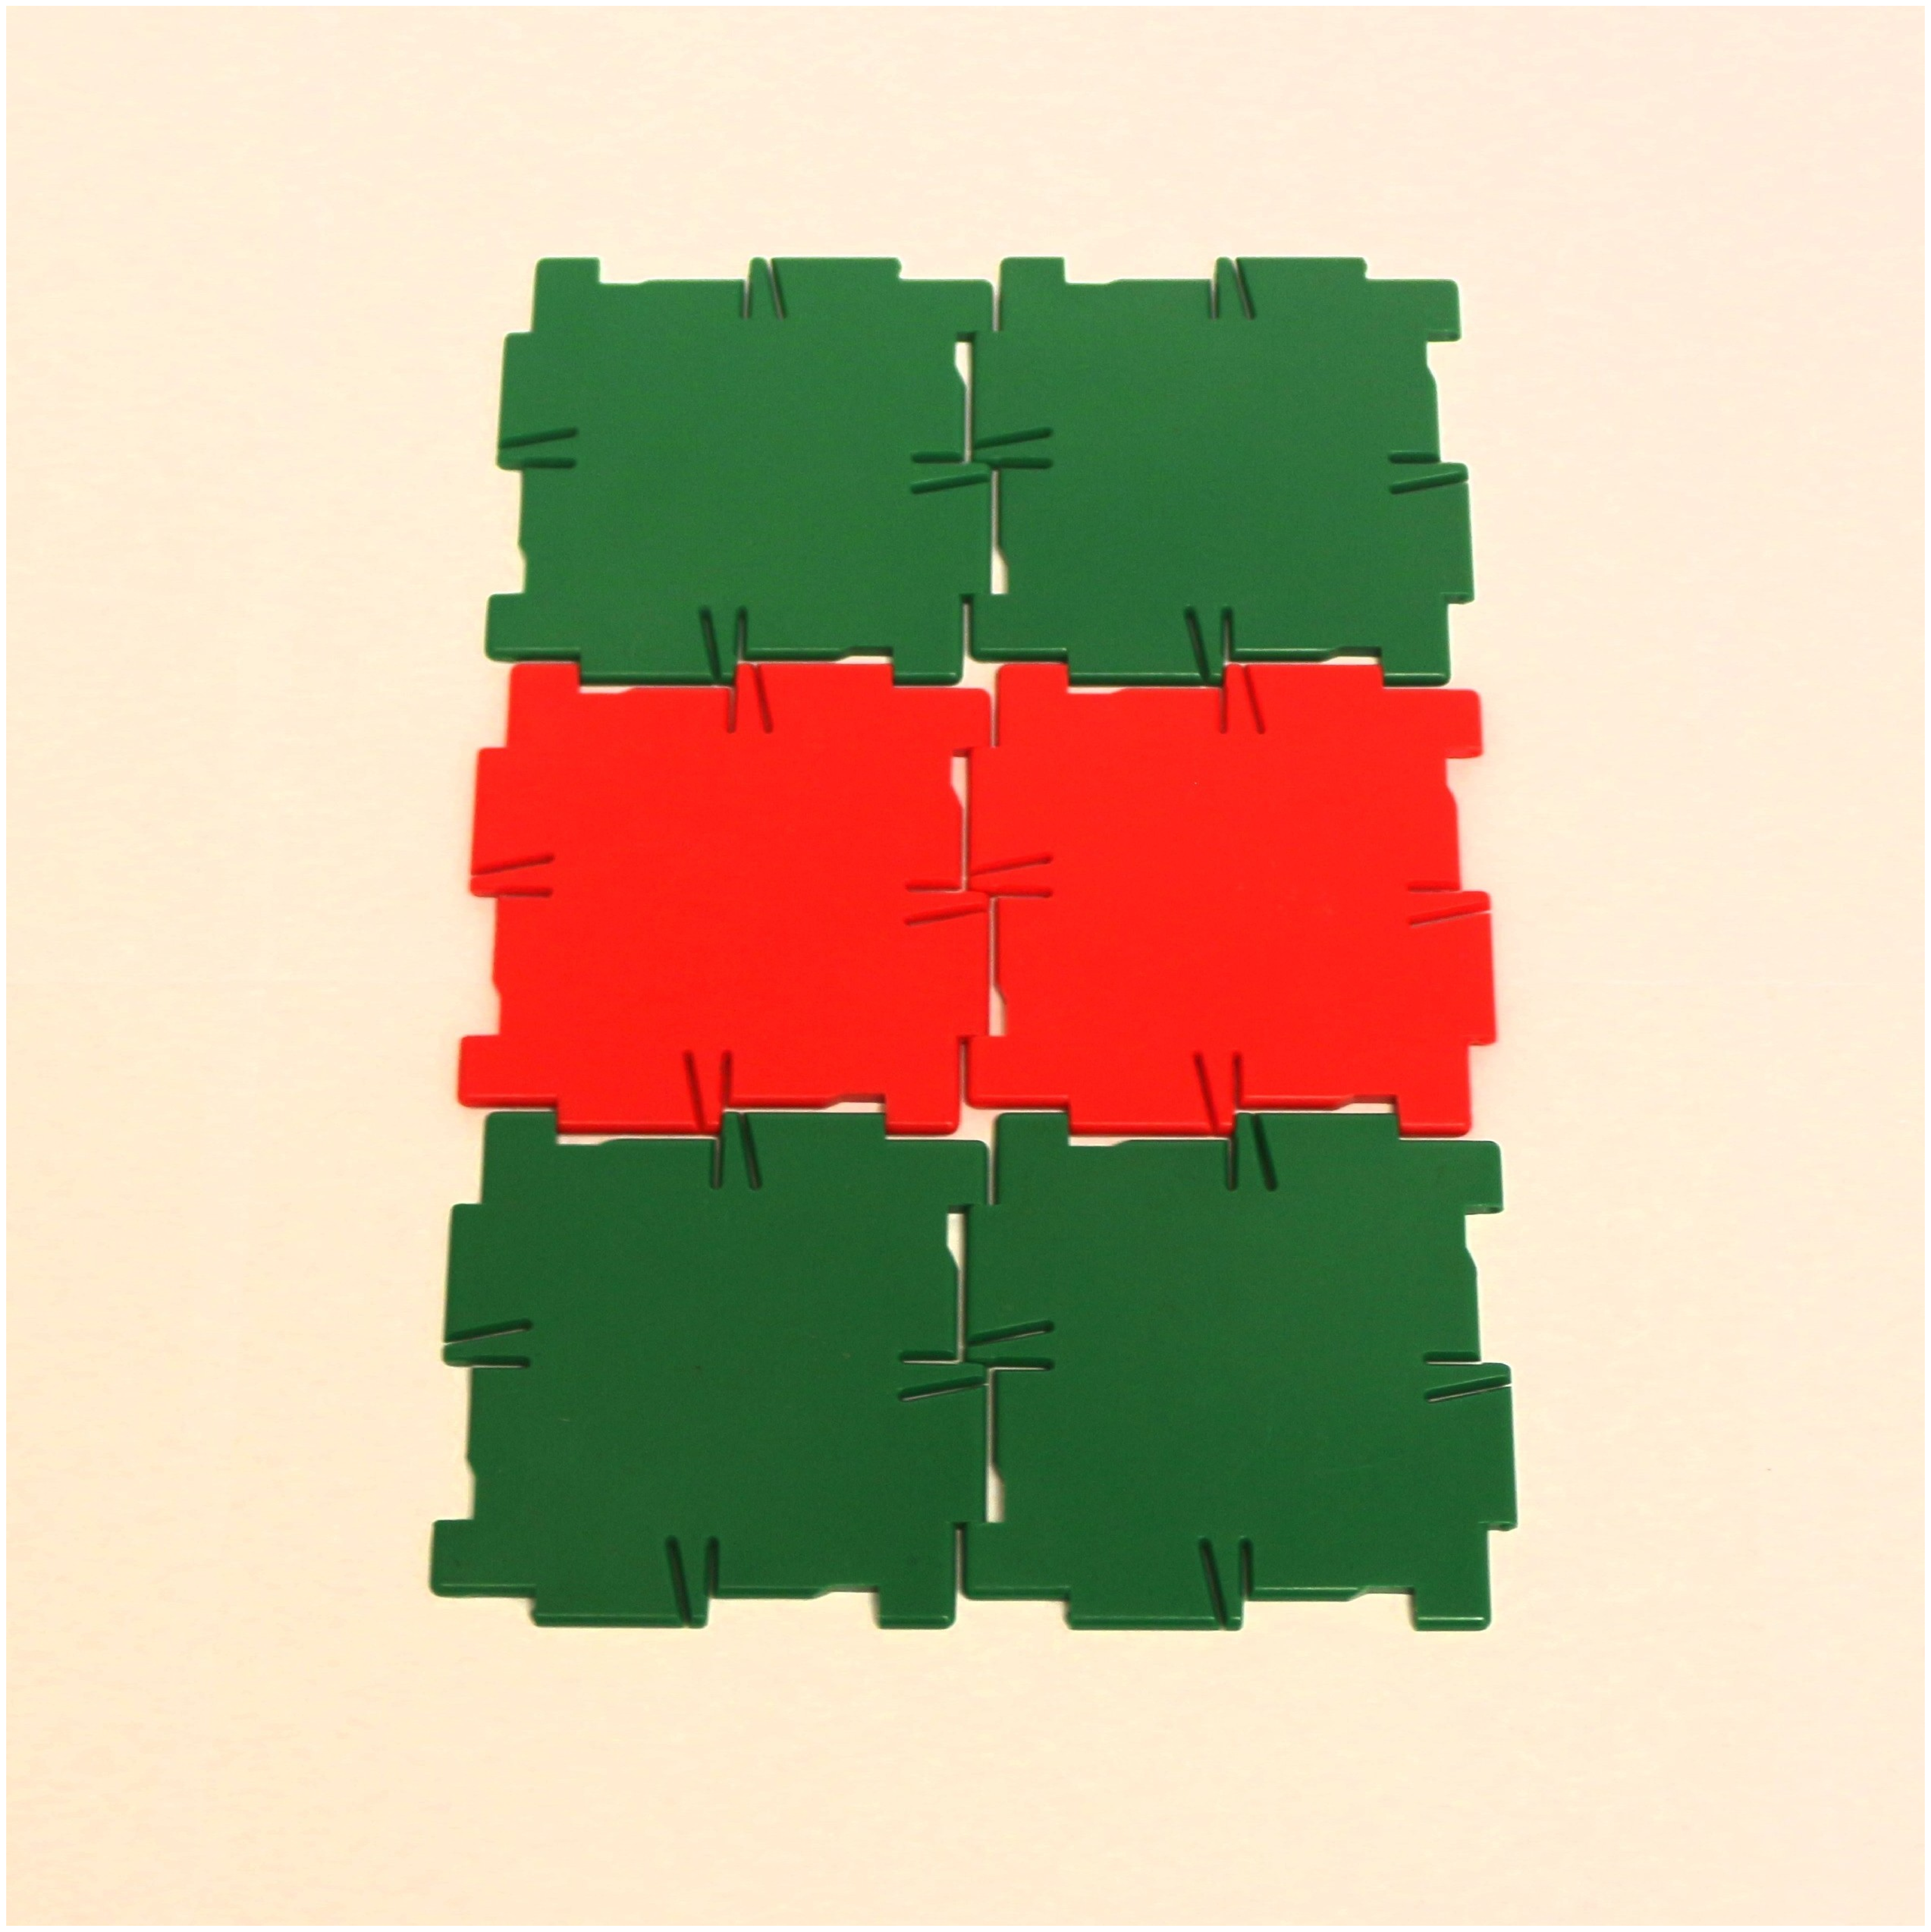
\includegraphics[width=0.3\textwidth]{images/G2x3_0.eps}
                %\caption{Chair}
                %\label{fig:Chair}
        %\end{subfigure}%
        %~ %add desired spacing between images, e. g. ~, \quad, \qquad etc.
          %(or a blank line to force the subfigure onto a new line)
        %\begin{subfigure}[b]{0.24\textwidth}
                
\includegraphics[width=0.3\textwidth]{images/G2x3_1.eps}
                %\caption{Boat}
                %\label{fig:Boat}
        %\end{subfigure}%
        %~ %add desired spacing between images, e. g. ~, \quad, \qquad etc.
          %(or a blank line to force the subfigure onto a new line)
        %\begin{subfigure}[b]{0.24\textwidth}
                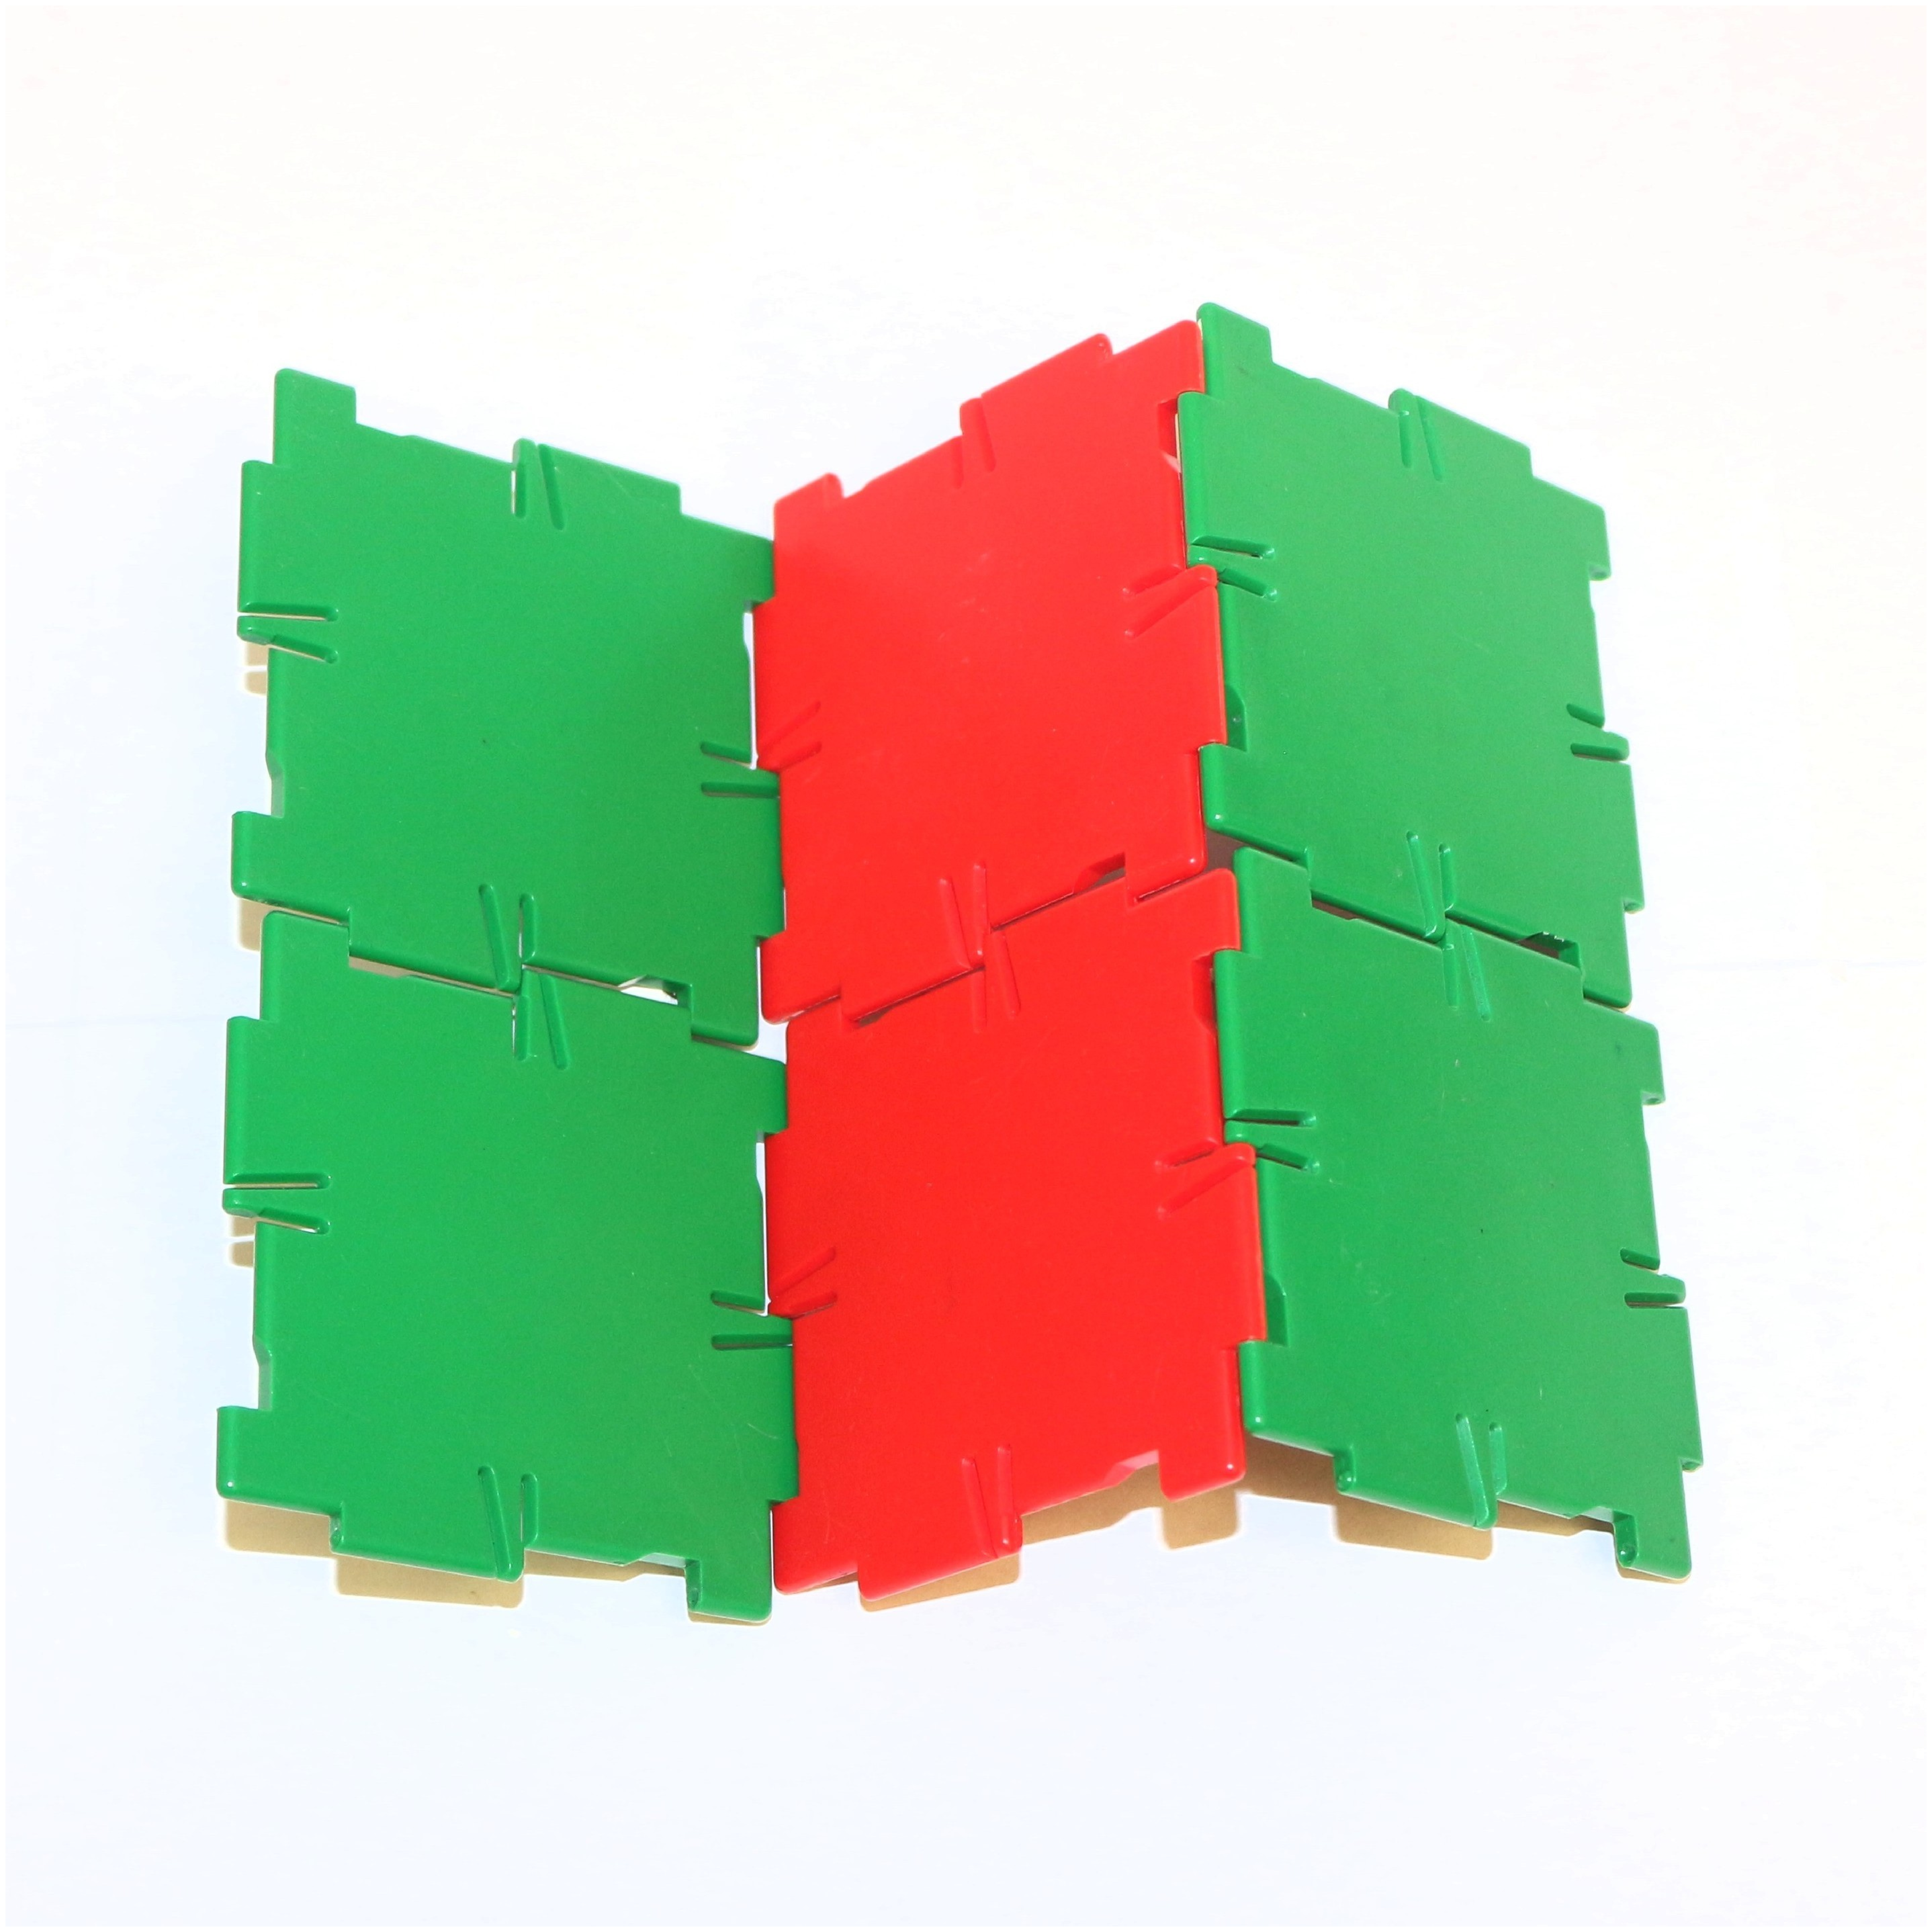
\includegraphics[width=0.3\textwidth]{images/G2x3_2.eps}
                %\caption{Twist Boat}
                %\label{fig:TwistBoat}
        %\end{subfigure}%


  %\includegraphics[scale=0.1, angle=0]{tetris.eps}
\caption{A linkage of 6 squares with configurations of different degrees of freedom.}
\label{fig:SixSq}
\end{figure}

As stated previously, we have not observed this type of behavior from any Building Game intermediates. This leads us to speculate that the degenerate nature of this example is down to an uncommon alignment of the hinged edges. Clearly, this linkage could never be an intermediate of a convex polyhedron. Perhaps the Building Game geometric configuration space has no singularities and is hence a manifold for all convex polyhedra.  

\subsection{Results}


\begin{figure}[ht]
\centering
  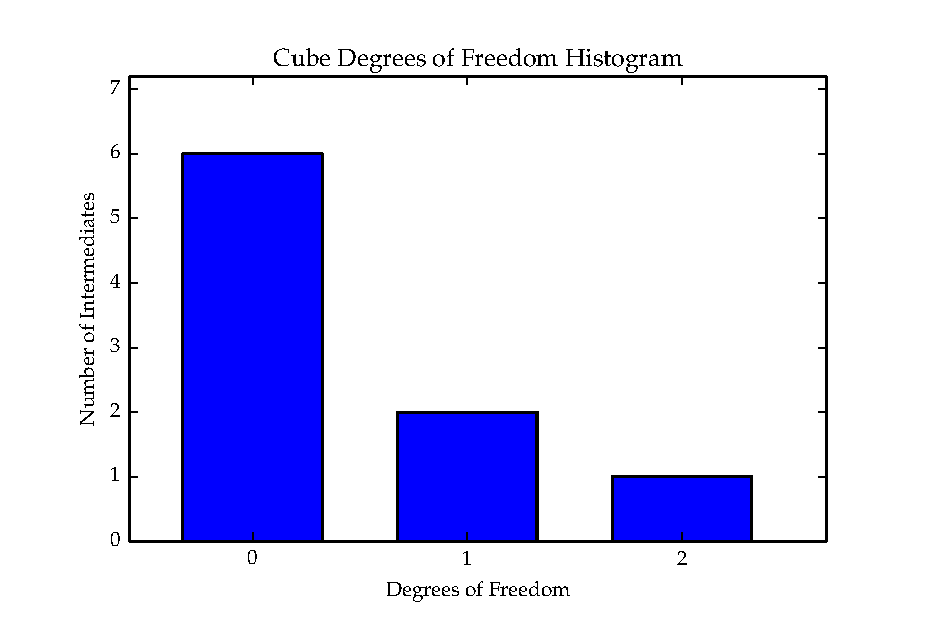
\includegraphics[scale=1.0, angle=0]{cube_dof_hist.eps}
\caption{Distribution of internal degrees of freedom amongst Cube intermediates.}
\label{fig:CubeDoFHist}
\end{figure}

\begin{figure}[ht]
\centering
  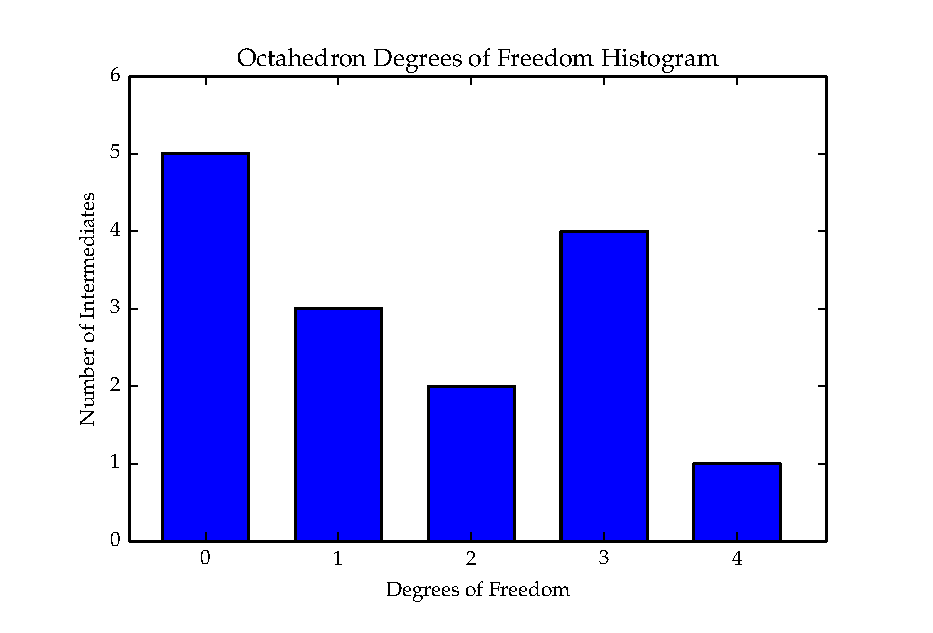
\includegraphics[scale=1.0, angle=0]{octahedron_dof_hist.eps}
\caption{Distribution of internal degrees of freedom amongst Octahedron intermediates.}
\label{fig:OctaDoFHist}
\end{figure}

\begin{figure}[ht]
\centering
  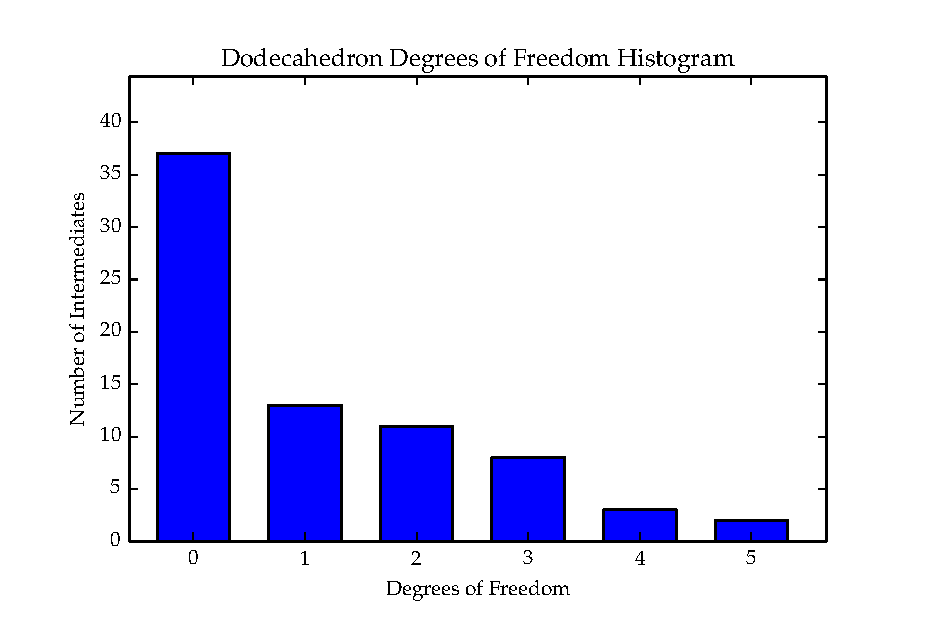
\includegraphics[scale=1.0, angle=0]{dodecahedron_dof_hist.eps}
\caption{Distribution of internal degrees of freedom amongst Dodecahedron intermediates.}
\label{fig:DodecDoFHist}
\end{figure}

\begin{figure}[ht]
\centering
  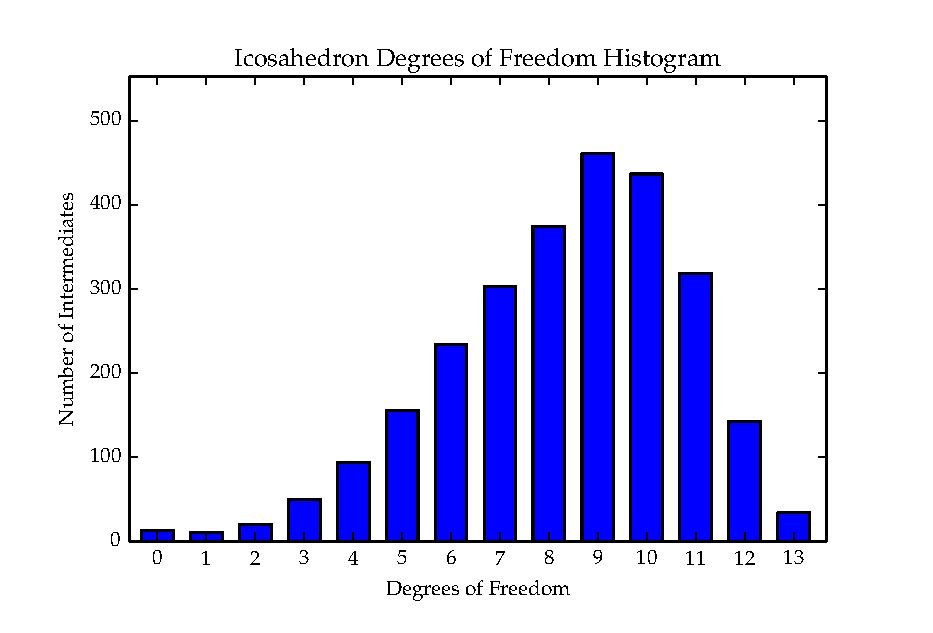
\includegraphics[scale=1.0, angle=0]{icosahedron_dof_hist.eps}
\caption{Distribution of internal degrees of freedom amongst Icosahedron intermediates.}
\label{fig:IcosaDoFHist}
\end{figure}

Using the Jacobian method for computing internal degrees of freedom, we have computed the number of degrees of freedom for all intermediates of the Platonic solids. Figures~\ref{fig:CubeDoFHist},~\ref{fig:OctaDoFHist},~\ref{fig:DodecDoFHist}, and~\ref{fig:IcosaDoFHist} are histograms of the number of internal degrees of freedom for the intermediates of each of the Platonic solids. We do not include the Tetrahedron, since it only has four intermediates and only the one composed of two triangles is not rigid. Interestingly, the cube and dodecahedron have a large number of rigid intermediates due  to the fact that their vertices are the rigid meeting of only three faces. The octahedron, with four faces meeting at each vertex has a more varied distribution of internal degrees of freedom. The icosahedron, however, has a very small number of rigid intermediates with some intermediates having as many as $13$ internal degrees of freedom. 

\begin{figure}[ht]
\centering
  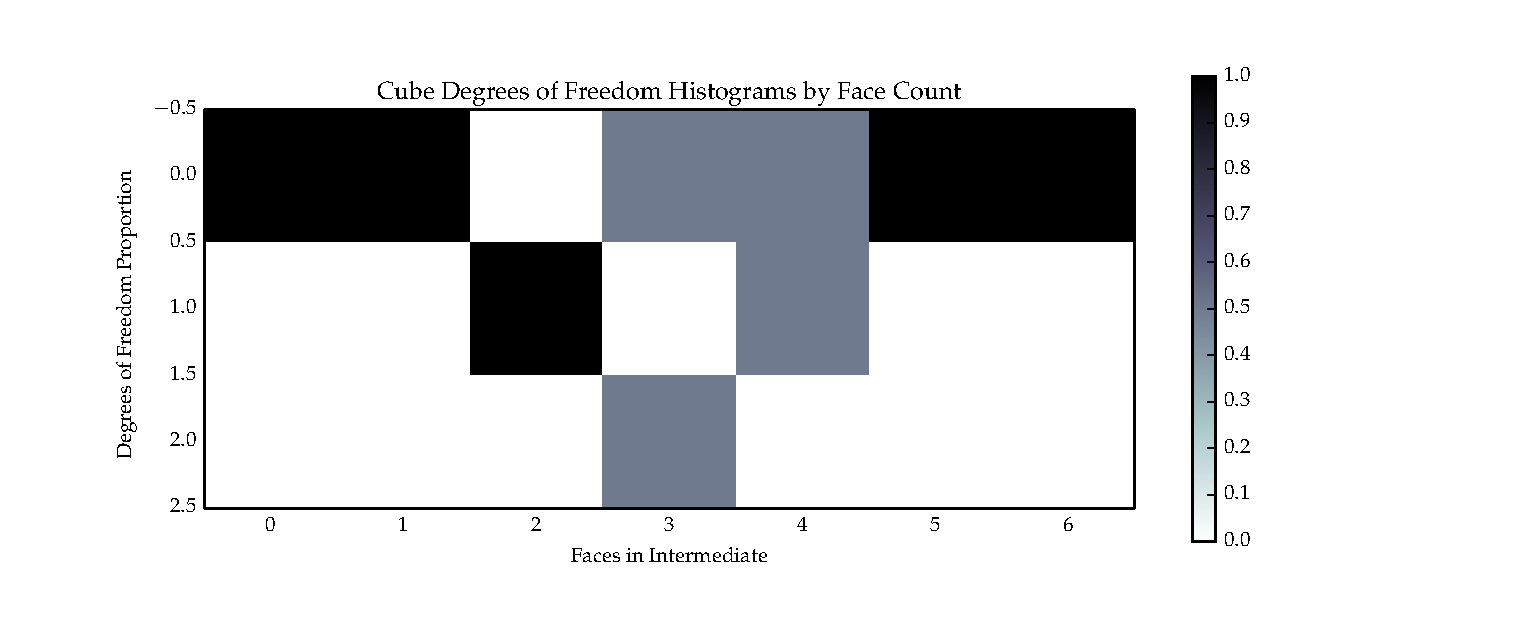
\includegraphics[scale=0.7, angle=0]{cube_dof_hist_facecount.eps}
\caption{Each vertical column gives a histogram of the number of internal degrees of freedom $k$-faced intermediates of the cube have.}
\label{fig:CubeDoFHistFC}
\end{figure}

\begin{figure}[ht]
\centering
  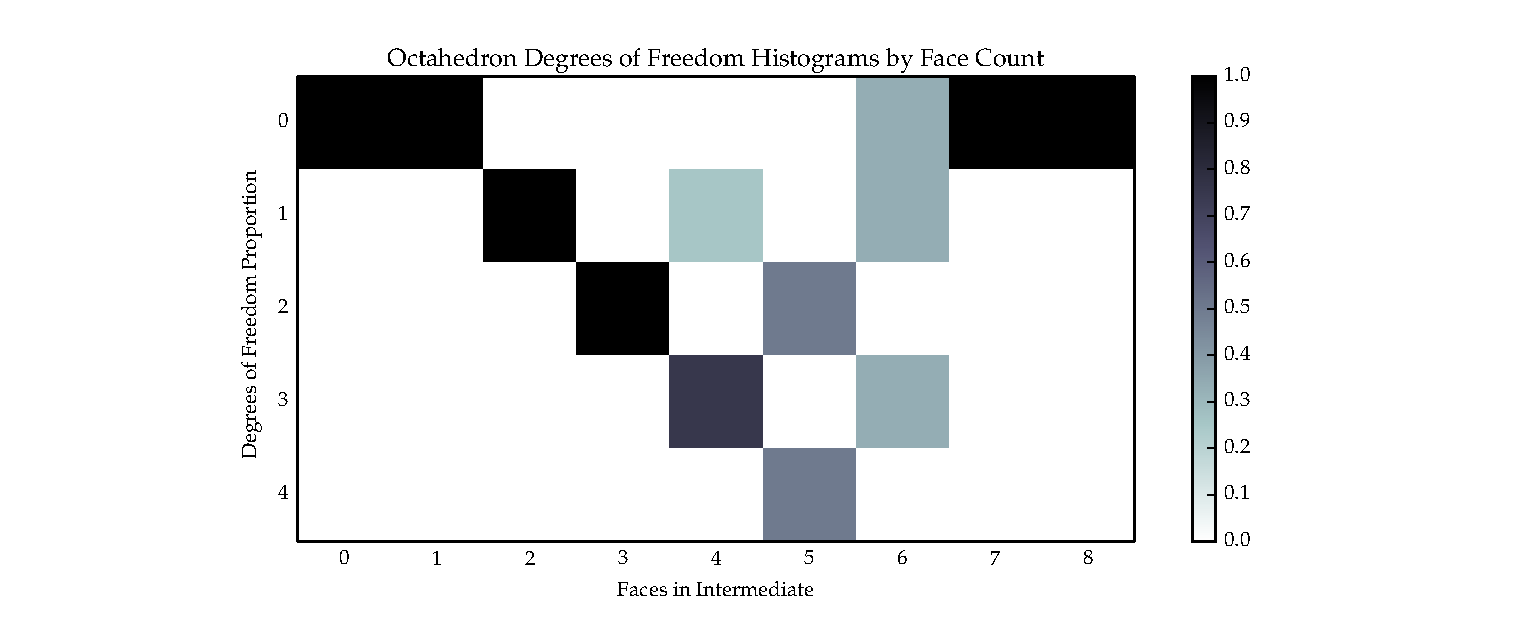
\includegraphics[scale=0.7, angle=0]{octahedron_dof_hist_facecount.eps}
\caption{Each vertical column gives a histogram of the number of internal degrees of freedom $k$-faced intermediates of Octahedron have.}
\label{fig:OctaDoFHistFC}
\end{figure}

\begin{figure}[ht]
\centering
  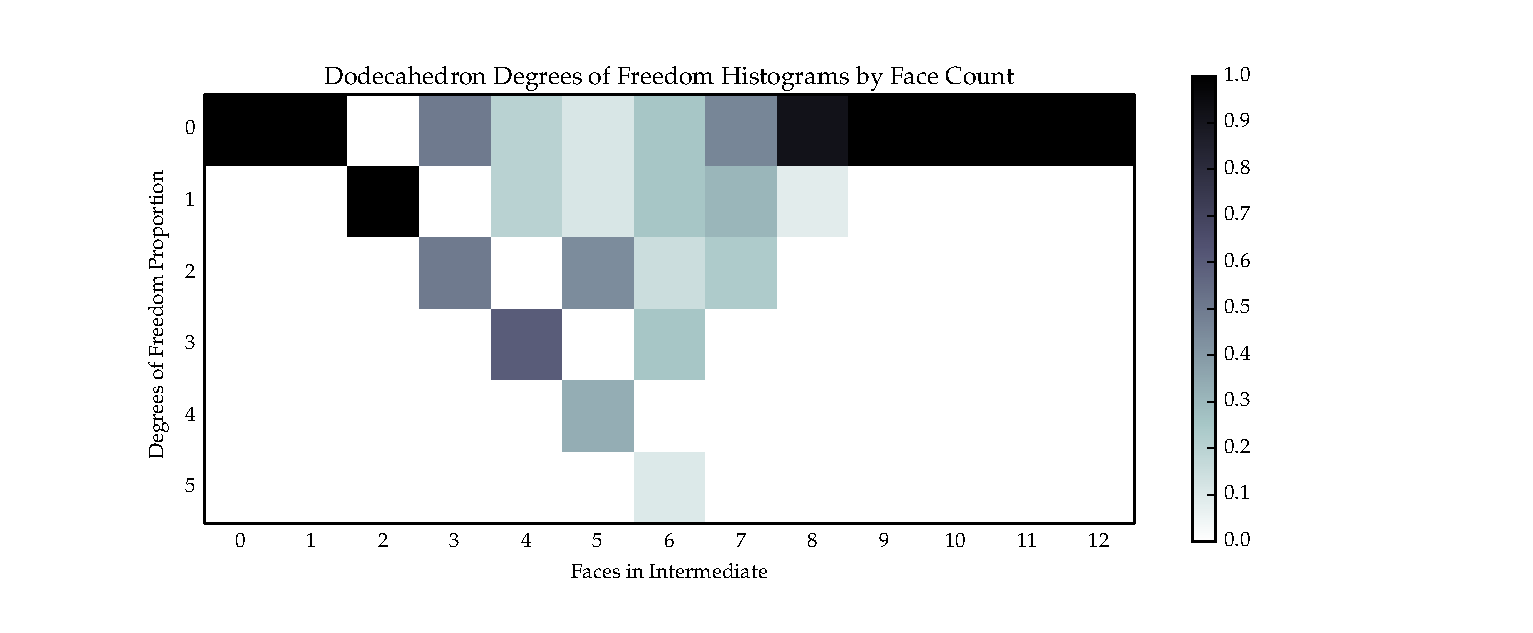
\includegraphics[scale=0.65, angle=0]{dodecahedron_dof_hist_facecount.eps}
\caption{Each vertical column gives a histogram of the number of internal degrees of freedom $k$-faced intermediates of the Dodecahedron have.}
\label{fig:DodecDoFHistFC}
\end{figure}

\begin{figure}[ht]
\centering
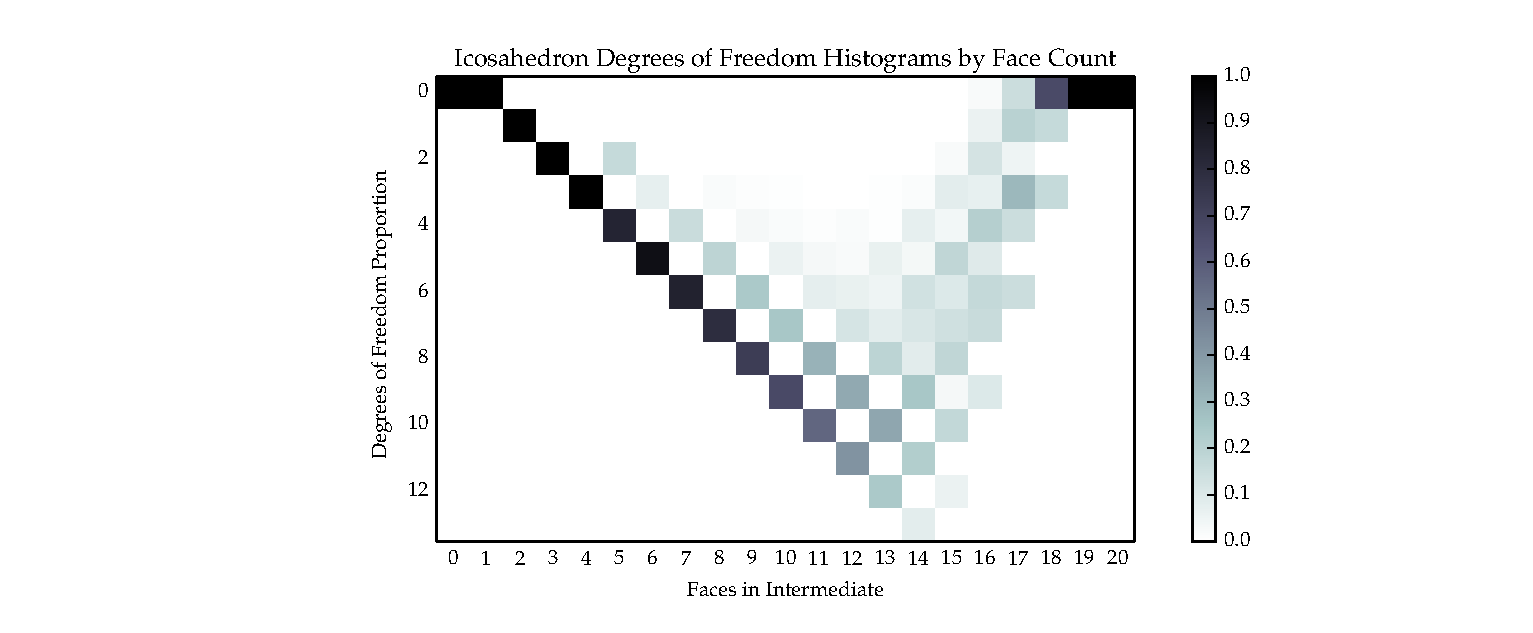
\includegraphics[scale=0.7, angle=0]{icosahedron_dof_hist_facecount.eps}
\caption{Each vertical column gives a histogram of the number of internal degrees of freedom $k$-faced intermediates of the icosahedron have.}
\label{fig:IcosaDoFHistFC}
\end{figure}

To provide a more detailed look at the distribution of internal degrees of freedom, figures~\ref{fig:CubeDoFHistFC},~\ref{fig:OctaDoFHistFC},~\ref{fig:DodecDoFHistFC}, and~\ref{fig:IcosaDoFHistFC} break down the previous histograms by the number of faces in the intermediate. Each column of the plots is a histogram for the number of internal degrees of freedom for the intermediates with that specific number of faces. The general theme seems to be that intermediates with almost all or almost none of their faces are most rigid and the intermediates with around half of the total possible faces have the most internal degrees of freedom. The most interesting case remains the icosahedron with a wide variation in internal degrees of freedom for most face counts.

\subsection{Explicit Removal of Trivial Degrees of Freedom}
\label{ssc:RemTrivDoF}
Since we are often solely interested the internal degrees of freedom, there are a few was to augment the constraint equations to mod out the translation or rotations causing the trivial degrees of freedom. One possible choice is to pick a face and constrain its vertex locations to match a fixed template. The corresponding constraint equations for fixing the $j$th face would be
\begin{align}
c_{fix}^{j,k,d}\left(z\right) &= v^{j,k}_d - \hat{v}^{j,k}_d \\
	\frac{\partial c_{fix}^{j,k,d}}{\partial z_i} &=
  	\begin{cases}
        	1 	& \text{if } z_i = v^{j,k}_d \\
   		0       & \text{else} 
  	\end{cases} 
\end{align}
for each dimension $d$ of each vertex $k$ of face $j$. For reasons we will explain in the next chapter, this may not always be an ideal choice if there is information other than the degrees of freedom we which to derive from the constraint equations.


An alternative that prevents translation, but does allow rotation is to fix the configuration's center of mass. 
\begin{align}
c_{com}^{d}\left(z\right) &= \sum_{j = 1}^{|F_x|}\sum_{k=1}^{s_{f_j}}v^{j,k}_d \\
	\frac{\partial c_{com}^{d}}{\partial z_i} &=
  	\begin{cases}
        	1 	& \text{if } z_i = v^{j,k}_d \\
   		0       & \text{else} 
  	\end{cases} 
\end{align}
This amounts to the sum over the $d$th entry of each vertex in the configuration.

%We consider the linkage of rigid 2-dimensional polygons in $\mathbb{R}^3$ by means of ideal hinges located at the edges of the polygons. In this way, by treating intermediates of our various models as such a linkage, we can compute the non-trivial degrees of freedom (DoF) each intermediate has. 

%Every linkage of this type has 6 trivial degrees of freedom: 3 corresponding to translational movement and 3 corresponding to rotational freedom. While these freedoms do change the orientation of the intermediate, they do not cause the faces to move relative to each other. For this reason, we label them as trivial degrees of freedom and focus on the calculation the remaining, non-trivial degrees of freedom. 

%For our purposes, we define the \textbf{degrees of freedom} of a configuration to be the difference between the number of parameters needed to specify a configuration in an ambient parameter space $\Omega$ and the number of independent constraints imposed upon the configuration as a function of these parameters. Consequently, the non-trivial degrees of freedom is the number of degrees of freedom minus the six trivial degrees of freedom. If the ambiant parameter space is $\mathbb{R}^N$ and there are $M$ constraint equations given by $\varphi : \mathbb{R}^N \to \mathbb{R}^M$, we find the degrees of freedom to be $N - \operatorname{rank}(\varphi)$ and the non-trivial degrees of freedom to be $N - \operatorname{rank}(\varphi) - 6$. Here we need $\varphi$ to be a smooth map so that the rank is well defined. Furthermore, we define the \textbf{configuration space} to be the subset of parameter space $\{\omega \in \Omega : \varphi(\omega) = 0\}$ upon which the contraints are satisfied.


%In our case, the location and orientation of each polygon in the linkage can be represented by a total of 6 parameters: 3 for location and 3 for roational orientation. Thus, the entire configuration of an intermediate $x$ can be represented in the parameter space $\mathbb{R}^{F_x\times6}$. With constraints corresponding to hinged connections we construct a function $\varphi$ which is zero if and only if the constraints are satisfied. Thus the configuration space is $\{z \in \mathbb{R}^{F_x\times6} : \varphi(z) =0\}$. As we will show below, the constraint equation $\varphi$ can be constructed as a polynomial which means that the configuration space (as the zero set of this polynomial) is an algebraic variety. 

% PARAGRAPH ON DIFFERENT DOF VALS AT DIFFERENT CONFIGS OF SAME INTERMEDIATE We refer to the embedded configuration of $x$ such that $x$ is a subset of the original polyhedron as the \textbf{canonical configuration}.


%The base constaints are put in place to fix one of the intermediate's faces in space to remove the 6 trivial degrees of freedom from the calculation. If $f_b$ is the face we wish to designate as the base we have the following $3\times s_b$ constraint equations
%\begin{align}
%\psi_{base}^{k,x}\left(\mathbf{v}\right)& = v^{b,k}_x - c^{b,k}_x \\
%\psi_{base}^{k,y}\left(\mathbf{v}\right)& = v^{b,k}_y - c^{b,k}_y \\
%\psi_{base}^{k,z}\left(\mathbf{v}\right)& = v^{b,k}_z - c^{b,k}_z
%\end{align}  
%for $k = 1,\dots,s_b$ and with $c^{b,k}_\bullet$ a known constant. The corresponding Jacobian calculation for each constraint equations is:
%\[
%\frac{\partial\psi_{base}^{k,\bullet}}{\partial v} =
%  \begin{cases}
%   1 & \text{if } v = v^{b,k}_\bullet \\
%   0       & \text{else} 
%  \end{cases}
%\]

%Edge length constraints enforce that the lengths of the edges of each face in an intermediate cannot change. Since there are $s_j$ edges for each face $f_j$ of intermediate $x$, there are $N_x$ corresponsing edge constraints. 
%\begin{align}
%\psi_{edge}^{j,k}\left(\mathbf{v}\right)& = \left|v^{j,k} - v^{j,k-1}\right|^2 - \ell_{j,k}^2 \\
%& = \left(v_x^{j,k} - v_x^{j,k-1}\right)^2 +\left(v_y^{j,k} - v_y^{j,k-1}\right)^2 +\left(v_z^{j,k} - v_z^{j,k-1}\right)^2 - \ell_{j,k}^2 
%\end{align}  
%for all $j: f_j \subset x$ and with the convention that $v^{j,0} \doteq v^{j,s_j}$ and $\ell_{j,k}$ is a known constant. The resulting partial derivatives are
%\[
%	\frac{\partial\psi_{edge}^{j,k}}{\partial v} =
%  	\begin{cases}
%        	2\left(v^{j,k}_\bullet-v^{j,k-1}_\bullet\right) 	& \text{if } v = v^{j,k}_\bullet \\
%   		-2\left(v^{j,k}_\bullet-v^{j,k-1}_\bullet\right) 	& \text{if } v = v^{j,k-1}_\bullet \\
%   		0       & \text{else} 
%  	\end{cases}
%\]
%--definiteion of 'base configuration'
%--representation of config space definition as system of constraint equations
%--solution of the constraint equations is a manifold except perhaps at some 'sp0ecial' configurations
%--define DoF as 6N - rank of the jacobian of the CEqs evaluated at the base config

%--go through computation of jacobian  




%\section{Cyclohexane Application}
%??Include??
%\subsection{Sachse Model}
%
%Around the turn of the century, it was thought that cyclohexane's carbon atoms must lie in a plane. A young German assistant, Hermann Sachse, had the idea that allowing the carbons to lie outside the plan could alleviate the angle strain. Inspired by polyhedral geometry, he templates and outlined methods for creating 3D models of the chair and boat configurations his new theory conceptualized. Figure~\ref{fig:sachse} shows a construction of these two models. Despite his best efforts, Sachse's ideas were not accepted by that chemistry community until after his death. 
%
%
%
%\begin{figure}
%        %\centering
%        %\begin{subfigure}[b]{0.24\textwidth}
%        %        \includegraphics[width=\textwidth]{chair_model_2.png}
%        %        \caption{Chair (top)}
%        %        \label{fig:CM1}
%        %\end{subfigure}%
%        %~ %add desired spacing between images, e. g. ~, \quad, \qquad etc.
%        %  %(or a blank line to force the subfigure onto a new line)
%        %\begin{subfigure}[b]{0.24\textwidth}
%        %        \includegraphics[width=\textwidth]{chair_model_1.png}
%        %        \caption{Chair (side)}
%        %        \label{fig:CM2}
%        %\end{subfigure}%
%        %~ %add desired spacing between images, e. g. ~, \quad, \qquad etc.
%        %  %(or a blank line to force the subfigure onto a new line)
%        %\begin{subfigure}[b]{0.24\textwidth}
%        %        \includegraphics[width=\textwidth]{boat_model_1.png}
%        %        \caption{Boat (top)}
%        %        \label{fig:BM1}
%        %\end{subfigure}%
%        %~ %add desired spacing between images, e. g. ~, \quad, \qquad etc.
%        %  %(or a blank line to force the subfigure onto a new line)
%        %\begin{subfigure}[b]{0.24\textwidth}
%        %        \includegraphics[width=\textwidth]{boat_model_2.png}
%        %        \caption{Boat (side)}
%        %        \label{fig:BM2}
%        %\end{subfigure}%
%        %\caption{Sachse Models}\label{fig:sachse}
%\end{figure}
%
% 
%\subsection{Idealized Constraint Model}\label{building_game}
%
%Withe the eclipsing and angle strains in mind, we heuristically define an idealized model of cyclohexane by imposing geometric constraints. Each configuration is represented by the 3-dimensional locations of the center of its carbon atoms and we explicitly parameterize these locations as $v_1, v_2, \dots, v_6$ where $v_k \in \mathbb{R}^3$. For ease of exposition, $v_0 \doteq v_6$ and $v_{-1} \doteq v_5$ are notationally identified. 
%
%First, we require that any two atoms sharing a bond have a known and fixed distance $\ell$ from each other. Since we can re-scale our coordinate system, we assume $\ell \doteq 1$. Additionally, we assume that the connectivity of the cyclohexane molecule is such that $v_k$ is bonded to $v_{k-1}$ for $k = 1,\dots,6$. This gives our first six constraint equations.
%$$0 = \varphi_{len}^k\left(v_{k-1},v_{k}\right) = \|v_k-v_{k-1}\| - 1 $$
%for $k = 1,\dots,6$. 
%
%Additionally, we impose constraints representing the angle strain. Since the carbon atoms have the lowest energy when their bonds are at tetrahedral angles, we fix the angle of each set of three adjacent carbons to be at the tetrahedral angle. This is equivalent to the six angle constraint equations 
%$$0 = \phi_{ang}^k\left(v_{k-2},v_{k-1},v_{k}\right) = \left(v_k-v_{k-1}\right)\cdot \left(v_{k-2}-v_{k-1}\right) + \frac{1}{3}$$
%for $k = 1,\dots,6$.
%
%\subsection{Degrees of Freedom in Ideal Model}
%
%The first step in answering these questions is determining whether there is any degrees of freedom to each configuration or whether they are rigid. This can be determined by using established theory on rigidity of linkages and degrees of freedom. By computing the Jacobian matrix $J(v)$ of the system of constraint equations, we have the following equation for the degrees of freedom for a constraint satisfying set of coordinates $v$.
%$$DoF(v) = 18 - rank(J(v))$$
%When the Jacobian is of full rank 18, none of the constraints are dependent on each other and thus there is no freedom in the linkage. When testing the chair, we found there to be $0$ degrees of freedom, meaning that it is impossible to make a transition from the chair to another configuration without breaking one or more of the constraint equations. For the boat, however, one degree of freedom was found. This result shows that it is possible to deform the boat continuously while satisfying the constraints, but it is not informative as to which configurations it can deform to. In particular, we are interested in finding a path to he twist boat or another boat configuration. 
%

%\section{Folding Configuration Space}
%???include??
%
%The number of degrees of freedom measures the rigidity of an intermediate, but some intermediates with the same number of degrees of freedom may have varying degrees of mobility. We seek to quantify an intermediate's mobility by the relative amount of movement the intermediate has for a small movement in its configuration space. Intermediates with the most mobility will move less than the less mobile intermediates for the same amount of movement in configuration space.  
%
%\subsection{Methods}
%% What is the configuration space?
%Each octahedron intermediate is composed of 8 equilateral triangles connected to each other along edges. We make the assumption that these triangles are rigid and cannot be deformed. Furthermore, when two triangles meet at an edge, they move relative to each other as if connected by an ideal hinge. Every configuration has 6 trivial degrees of freedom corresponding to the 3 translation degrees of freedom and the 3 rotational degrees of freedom. Since we are interested in the motion of an intermediate's faces relative to each other, we remove these trivial degrees of freedom by picking a single face to fix in space. Depending on the connectivity of the triangle's edges, an intermediate 
%may still have degrees of freedom. The Octahedron intermediate (83), being a convex polyhedron, is rigid and has no non-trivial degrees of freedom as given by Cauchy's Theorem. However, this is not the case for most of the intermediates.
%
%We formalize the concept of the configuration space, by defining it to be the subset of an ambient parameter space that satisfies constraint equations that correspond to our assumptions. Since the are 8 faces in each intermediate and each face has 3 vertices each with 3 spacial coordinates (x,y,z), we use $\mathbb{R}^{8\times 3 \times 3} = \mathbb{R}^{72}$ as our ambient space. We then have 3 types of constraint equations: base face constraints, rigid face constraints, and hinge constraints. Every admissible configuration of an intermediate will be a point in $\mathbb{R}^{72}$ that satisfies the constraint equations and any admissible movement of a configuration (if possible) is a continuous movement in the subset of $\mathbb{R}^{72}$ where these constraints are satisfied. 
%
%Since our constraint equations can all be expressed as polynomials, the configuration space which is the corresponding solution set is an Algebraic variety. The number of degrees of freedom of a configuration is the local dimension of this algebraic variety as a subset of $\mathbb{R}^{72}$. In the case of octahedron intermediates, the number of degrees of freedom is not an informative way of classifying which intermediates are dominant as intermediates $1-11$ have $7$ degrees of freedom, $12-33$ have $5$, $34-65$ have $3$, $66-82$ have $1$ and the Octahedron (83) and Boat (84) have $0$ degrees of freedom. Thus, a different measure the mobility of a configuration is required to differentiate intermediates. It is important to note that degrees of freedom of in intermediate can theoretically change based on the region of configuration space. However, in practice we have not observed an intermediate's degrees of freedom change in this way. 
%
%We define the \textit{canonical configuration} of an intermediate, to be that in which each hinge forms a $180^\circ$ angle when the hinge does not have a vertex connection at either end and in the case of a closed vertex, the hinge's angle corresponds to the Octahedral angle. In cases where the intermediate cannot form an octahedron, we can use the Boat configuration's angles instead.
%
%% How do we move in the configuration space?
%Given a particular configuration $X$, if we wish to make a small move in configuration space, we first find the null space of the Jacobian matrix of the constraint equations. Since this null space corresponds to the directions in which the constraint equations are not changing, the constraints will remain satisfied. The null space can be represented by an orthonormal basis $N \in \mathbb{R}^{72\times d}$, where $d$ is the number of degrees of freedom of the configuration. Then, by taking a small step of size $\epsilon$ in each of the $d$ directions we get the configurations $X + \epsilon N_{\cdot,k}$. 
%% How do we measure the magnitude of a movement in configuration space?
%
%We define the \textit{mobility} of a configuration to be the $L^2$ norm of the gradient of the configuration space. To approximate this, we measure the mean squared distance between each point of $X$ and $X \pm \epsilon N_{\cdot,k}$ in each of the $d$ directions of $N$, take the norm, and divide by $\epsilon$. This is given by Equation~\ref{eq:r1} where $\triangle_f$ refers to the $f$th face of the intermediate and $r\left(X\right)$ is the point we are integrating over and $r\left(X+\sigma \epsilon N_{\cdot,k}\right)$ is the corresponding point in the altered configuration. 
%
%
%To explicitly define the rotation and translation of each face by the movement in configuration space, we use the algorithm given by Arun et al~\cite{Arunetal1987}. Given two sets of points $P,P' \in \mathbb{R}^{3\times n}$ in 3D space, the algorithm finds the rotation matrix $R$ and translation vector $b$ minimizing the least squares error of $P' \approx R P + b$. By using the three vertices of face $f$ as $P$ and their perturbed values as $P'$, we use this algorithm to find the rotation matrix $R_f$ and translation vector $b_f$ to describe the rigid movement of face $f$ in the configuration space. This leads to the formulation in Equation~\ref{eq:r3}.  
%\begin{figure}[h]
%  %\centering
%  %\includegraphics[width=0.61\textwidth]{triangle_fig.png}
%  %\caption{Coordinates of rotated triangle for integration.}
%  \label{fig:tri}
%\end{figure}
%
%To make this integral easier to solve, we introduce a change of variables that enables us to integrate in the $x-y$ plane. If the the original triangle $f$ has vertices of $a', b',$ and $c'$, we consider the triangle with vertices at the coordinates $a = (0,0,0), b = (|a-b|,0,0),$ and $c = (\alpha,\beta,0)$ as seen in Figure~\ref{fig:tri}. Here, the choices $\alpha = \frac{|a-b|^2 + |a-c|^2 - |b-c|^2 }{2|a-b|}$ and $\beta = \sqrt{|a-c|^2-\alpha^2}$ yield a triangle congruent to the original. Using the Arun et al~\cite{Arunetal1987} algorithm again, we find the rotation matrix $S_f$ and translation vector $c_f$ that gives $[a',b',c'] = S_f[a,b,c] + c_f$. Using this we perform a change of variables and integrate over $s$ and $t$. This results in an simple double integral over a quadratic function of $s$ and $t$ with constants $u,v,w \in \mathbb{R}^3$ as seen in Equation~\ref{eq:r5}.
%{\tiny
%\begin{align}
%\mathcal{R}\left(x\right) &= \frac{1}{\epsilon}\left(\sum_{k=1}^d \sum_{f=1}^8 \int_{\triangle_f}\left|\frac{r\left(x+\epsilon N_{\cdot,k}\right) - r\left(x\right)}{2\sqrt{3}}\right|^2\right)^{\frac{1}{2}} \label{eq:r1}  \\
%&= \frac{1}{2\sqrt{3}\epsilon}\left( \sum_{k=1}^d \sum_{f=1}^8 \int_{\triangle_f}\left|R_fr+b_f - r\right|^2\right)^{\frac{1}{2}} \label{eq:r2} \\
%&= \frac{1}{2\sqrt{3}\epsilon}\left( \sum_{k=1}^d \sum_{f=1}^8 \int_{\triangle_f}\left|\left(R_f-I\right)r+b_f\right|^2\right)^{\frac{1}{2}} \label{eq:r3} \\
%&= \frac{1}{2\sqrt{3}\epsilon}\left( \sum_{k=1}^d \sum_{f=1}^8 \int_{0}^{\beta}\int_{\frac{\alpha}{\beta}t}^{|a-b| + \frac{\alpha- |a-b|}{\beta}t}\left|\left(R_f-I\right)\left(S_f\begin{bmatrix} s \\[0.3em] t \\[0.3em] 0 \end{bmatrix} + c_f\right)+b_f\right|^2ds dt\right)^{\frac{1}{2}} \label{eq:r4} \\
%&= \frac{1}{2\sqrt{3}\epsilon}\left( \sum_{k=1}^d \sum_{f=1}^8 \int_{0}^{\beta}\int_{\frac{\alpha}{\beta}t}^{|a-b| + \frac{\alpha- |a-b|}{\beta}t}\left|u + sv + tw\right|^2ds dt\right)^{\frac{1}{2}} \label{eq:r5} 
%\end{align} 
%}    
%% Why does the choice of the base constraint matter and how do we deal with it?
%
%Unfortunately, the particular choice of base face affects the mobility. To rectify this bias, we compute the mobility with each of the eight faces as the base and take the average. This gives the final mobility in Equation~\ref{eq:r6}. 
%{\tiny
%\begin{align}
%\mathcal{R} &= \frac{1}{8}\sum_{g=1}^8\mathcal{R}_g \\
%&= \frac{1}{16\sqrt{3}\epsilon}\sum_{g=1}^8\left( \sum_{k=1}^d \sum_{f=1}^8 \int_{0}^{\beta}\int_{\frac{\alpha}{\beta}t}^{|a-b| + \frac{\alpha- |a-b|}{\beta}t}\left|u + sv + tw\right|^2ds dt\right)^{\frac{1}{2}} \label{eq:r6} 
%\end{align}     
%}
%
%\section{Results}
%
%Mobility was computed for all octahedral intermediates in their canonical configuration. The perturbation parameter $\epsilon = 10^{-6}$ was selected, but the mobility showed to be robust to both smaller and larger values. Figure~\ref{fig:t1} outlines the results. From these calculations, it is clear that while mobility is highly correlated to degrees of freedom, mobility gives additional information about an intermediate's configuration space. Interestingly, all nets had the same mobility. Similarly, the symmetric pairs (14,16), (15,18), (19,20), (34,38), and (36,39) have matching mobility values. Of the intermediates with 5 degrees of freedom, 19 and 20 had the lowest mobility and 17 had the highest. As for intermediates with 3 degrees of freedom, 35 was the least mobile and 37 was the most mobile.        
%
%\begin{figure}[h!]
%\label{fig:t1}
%%\centering
%\scalebox{.9}{
%\begin{tabular}{ l | c }
%  Intermediate & Mobility  \\
%  \hline\hline
%1 &  0.20518 \\
%2 &  0.20518 \\
%3 &  0.20518 \\
%4 &  0.20518 \\
%5 &  0.20518 \\
%6 &  0.20518 \\
%7 &  0.20518 \\
%8 &  0.20518 \\
%9 &  0.20518 \\
%10 & 0.20518 \\
%11 & 0.20518 \\\hline
%12 & 0.18376 \\
%13 & 0.18313 \\
%14 & 0.18249 \\
%15 & 0.18171 \\
%16 & 0.18249 \\
%17 & 0.18634 \\
%18 & 0.18171 \\
%19 & 0.18102 \\
%20 & 0.18102 \\
%21 & 0.18255 \\
%22 & 0.18485 \\\hline
%34 & 0.14487 \\
%35 & 0.14350 \\
%36 & 0.14530 \\
%37 & 0.14973 \\
%38 & 0.14487 \\
%39 & 0.14530 \\\hline
%66 & 0.07954 \\\hline
%83 & 0.00000 \\
%\end{tabular}
%}
%%\caption{A table with the mobility of octahedral intermediates.}
%\end{figure}

\clearpage{\pagestyle{empty}\cleardoublepage}

\chapter{Processes in Constraint Spaces}
\section{Constrained Dynamics}

Sometimes we are interested in more than simply the number of degrees of freedom a particular configuration has. To explore the configuration space, find similarities between different configurations, analyze the geometric configuration space's topology, or compute other relevant statistics, it can be useful to compute dynamic processes on the geometric configuration space. There are clear computational challenges to computing such dynamics due to computational handling of constraints, the lack of an explicit parameterizations, and the fact that geometric configuration space is often of much smaller dimension than the ambient space it sits in.

%Constraint algorithms have been widely studied for use in molecular dynamic simulations. Many  methods use a two stage scheme in which the unconstrained dynamics are first used to evolve the system to an intermediary configuration $\hat{z}_{n+1}$ based on the previous configuration $z_n$. In the second stage, Lagrange multipliers are used to correct $\hat{z}_{n+1}$ to a new configuration $z_{n+1}$ which satisfies the constraints. Previously, we used the SHAKE algorithm--which employs this two stage philosophy--to examine a constraint space used to model the configurations of cyclohexane~\cite{Pandey2014}. 

%Constraint algorithms can be used to compute various statistics of the configuration space. For example, the relative volume of different regions of configuration space can be empirically estimated. Additionally, if we have soft constraints, such as preferred angles between faces, we can institute cost functions on the configuration space with configurations having more favorable angles having a lower cost. Whether physically or artificially motivated, such cost functions can be treated as potential energy functions which can imply specific dynamics. Under this set of dynamics, quantities such as the average or minimum energies may be of interest. 

%We may also be interested in the behavior of a small part of the configuration as it undergoes constrained dynamics. For instance, suppose we are interested in the tendency for two edges on distinct faces to come together and form a new connection. By looking at the distance between these edges, we can measure how frequently this event happens and the probability that it will occur before another event of interest. This is similar to the exit time problem for diffusion and may provide a physically motivated evaluation tool for the appropriateness of our transition rules we adopt in our models. 


%\subsection{Cyclohexane Application}

%??include??

%\label{introduction}
%Cyclohexane is a molecule composed of six carbon atoms and twelve hydrogen atoms. The carbon atoms are connected in a ring with two hydrogen atoms attaching to each carbon. Since each carbon has four bonds, the energetically preferred bond spacing is at tetrahedral angles. While this preference dictates much of the cyclohexane structure, there are several structurally distinct conformations the molecule can take. 
%
%Of the many forces acting on the cyclohexane molecule, we focus on three. \textbf{Eclipsing strain} refers to the force between the carbon atoms that prevents them from getting too close to each other. This imposes a preferred distance between each pair of bonded atoms. Second, \textbf{angle strain} corresponds to the carbon atom's four bonds trying to spread apart from each other. As mentioned before, tetrahedral angles are preferred. Finally, \textbf{steric crowding} is similar to eclipsing strain, but the eclipsing in this case is between the hydrogen atoms bonded to the carbons.
%
%\subsubsection{Configurations}
%
%Due to the aforementioned forces, there are a variety of frequently observed configurations with geometries that alleviate these strains to varying amounts. 
%
%The lowest energy configuration is the \textbf{chair}. With the absence of both angle and eclipsing strain, the chair only has a small amount of steric strain. 
%
%Another well studied configuration is the \textbf{boat}. With two sets of parallel carbons arranged in a planar rectangular structure, the remaining two carbon atoms sit at opposite ends slightly above the plain. The structure resembles the bow and stern of a boat. Despite having little angle strain, it does have some steric crowding between the hydrogen atoms at the ends of the boat as well as some eclipsing stain.
%
%
%
%\begin{figure}
%        %\centering
%%        \begin{subfigure}[b]{0.24\textwidth}
%%                \includegraphics[width=\textwidth]{pv_chair_1.png}
%%                %\caption{Chair}
%%                %\label{fig:Chair}
%%        \end{subfigure}%
%%        ~ %add desired spacing between images, e. g. ~, \quad, \qquad etc.
%%          %(or a blank line to force the subfigure onto a new line)
%%        \begin{subfigure}[b]{0.24\textwidth}
%%                \includegraphics[width=\textwidth]{pv_boat_1.png}
%%                %\caption{Boat}
%%                %\label{fig:Boat}
%%        \end{subfigure}%
%%        ~ %add desired spacing between images, e. g. ~, \quad, \qquad etc.
%%          %(or a blank line to force the subfigure onto a new line)
%%        \begin{subfigure}[b]{0.24\textwidth}
%%                \includegraphics[width=\textwidth]{pv_twist_boat_2.png}
%%                %\caption{Twist Boat}
%%                %\label{fig:TwistBoat}
%%        \end{subfigure}%
%%        ~ %add desired spacing between images, e. g. ~, \quad, \qquad etc.
%%          %(or a blank line to force the subfigure onto a new line)
%%        \begin{subfigure}[b]{0.24\textwidth}
%%                \includegraphics[width=\textwidth]{pv_twist_chair_2.png}
%%                %\caption{Twist Chair}
%%                %\label{fig:TwistChair}
%%        \end{subfigure}%
%%
%%        \begin{subfigure}[b]{0.24\textwidth}
%%                \includegraphics[width=\textwidth]{pv_chair_2.png}
%%                %\caption{Chair}
%%                %\label{fig:Chair}
%%        \end{subfigure}%
%%        ~ %add desired spacing between images, e. g. ~, \quad, \qquad etc.
%%          %(or a blank line to force the subfigure onto a new line)
%%        \begin{subfigure}[b]{0.24\textwidth}
%%                \includegraphics[width=\textwidth]{pv_boat_2.png}
%%                %\caption{Boat}
%%                %\label{fig:Boat}
%%        \end{subfigure}%
%%        ~ %add desired spacing between images, e. g. ~, \quad, \qquad etc.
%%          %(or a blank line to force the subfigure onto a new line)
%%        \begin{subfigure}[b]{0.24\textwidth}
%%                \includegraphics[width=\textwidth]{pv_twist_boat_1.png}
%%                %\caption{Twist Boat}
%%                %\label{fig:TwistBoat}
%%        \end{subfigure}%
%%        ~ %add desired spacing between images, e. g. ~, \quad, \qquad etc.
%%          %(or a blank line to force the subfigure onto a new line)
%%        \begin{subfigure}[b]{0.24\textwidth}
%%                \includegraphics[width=\textwidth]{pv_twist_chair_1.png}
%%                %\caption{Twist Chair}
%%                %\label{fig:TwistChair}
%%        \end{subfigure}%
%%
%%        \begin{subfigure}[b]{0.24\textwidth}
%%                \includegraphics[width=\textwidth]{pv_chair_3.png}
%%                \caption{Chair}
%%                \label{fig:Chair}
%%        \end{subfigure}%
%%        ~ %add desired spacing between images, e. g. ~, \quad, \qquad etc.
%%          %(or a blank line to force the subfigure onto a new line)
%%        \begin{subfigure}[b]{0.24\textwidth}
%%                \includegraphics[width=\textwidth]{pv_boat_3.png}
%%                \caption{Boat}
%%                \label{fig:Boat}
%%        \end{subfigure}%
%%        ~ %add desired spacing between images, e. g. ~, \quad, \qquad etc.
%%          %(or a blank line to force the subfigure onto a new line)
%%        \begin{subfigure}[b]{0.24\textwidth}
%%                \includegraphics[width=\textwidth]{pv_twist_boat_3.png}
%%                \caption{Twist Boat}
%%                \label{fig:TwistBoat}
%%        \end{subfigure}%
%%        ~ %add desired spacing between images, e. g. ~, \quad, \qquad etc.
%%          %(or a blank line to force the subfigure onto a new line)
%%        \begin{subfigure}[b]{0.24\textwidth}
%%                \includegraphics[width=\textwidth]{pv_twist_chair_3.png}
%%                \caption{Twist Chair}
%%                \label{fig:TwistChair}
%%        \end{subfigure}%
%%
%%
%%        \caption{Cyclohexane Configurations}\label{fig:animals}
%\end{figure}
%
%
%Besides the chair and boat, there are a few intermediate configurations that cyclohexane assumes as when it transitions between the chair and boat. The aptly named \textbf{twist boat} is similar to the boat, but some of the carbons are rotated from the rest of the molecule. Due to this twisting, the twist boat actually has a lower energy than the boat as the hydrogen atoms at the bow and stern are no longer aligned. Interestingly, the boat can transition via the twist boat to a second boat configuration in which the bow and stern atoms are different, but with an otherwise indistinguishable geometry. As part of the boat's transition to the chair, the \textbf{twist chair} is another distinguished configuration. Having large angle and eclipsing strains, the twist boat represents somewhat of an energy barrier between the chair and boat.  
%
%
%\subsubsection{Finding Intermediate Coordinates}
%
%Since any configuration has an infinitude of equivalent configurations given by rotations and translations, we fix the first three atoms $v_1, v_2,v_3$, at positions $c_1, c_2, c_3$ that satisfy the length and angle constraints. These account for nine of the twenty-one total constraint equations. 
%
%We wish to examine each of the four cyclohexane configurations to verify if they satisfy these constraints, but to do so, an explicit representation of the coordinates of each configuration is required. Since we know from Sachse's model that the boat and chair have a special polyhedral representation, geometry enables us to find such coordinates. We pick the $c_1 = \left(-\sqrt{\frac{2}{3}},0,\sqrt{\frac{1}{3}}\right)$, $c_2 = \left(0,0,0\right)$, $c_3  = \left(\sqrt{\frac{2}{3}},0,\sqrt{\frac{1}{3}}\right)$, and solve for the following coordinates.
%
%\begin{align*}
%v_1^{(chair)} &= \left(-\sqrt{\frac{2}{3}},0,\sqrt{\frac{1}{3}}\right) &= v_1^{(boat)} &= \left(-\sqrt{\frac{2}{3}},0,\sqrt{\frac{1}{3}}\right) \\
%v_2^{(chair)}  &= \left(0,0,0\right) &= v_2^{(boat)}  &= \left(0,0,0\right) \\
%v_3^{(chair)}  &= \left(\sqrt{\frac{2}{3}},0,\sqrt{\frac{1}{3}}\right) &= v_3^{(boat)}  &= \left(\sqrt{\frac{2}{3}},0,\sqrt{\frac{1}{3}}\right) \\
%v_4^{(chair)}  &= \left(\sqrt{\frac{2}{3}},\sqrt{\frac{2}{3}},2\sqrt{\frac{1}{3}}\right) &= v_4^{(boat)}  &= \left(\sqrt{\frac{2}{3}},\sqrt{\frac{2}{3}},2\sqrt{\frac{1}{3}}\right) \\
%v_5^{(chair)}  &= \left(0,\sqrt{\frac{2}{3}},\sqrt{3}\right) & v_5^{(boat)}  &= \left(0,\frac{5}{3}\sqrt{\frac{2}{3}},\frac{5}{3}\sqrt{3}\right) \\
%v_6^{(chair)}  &= \left(-\sqrt{\frac{2}{3}},0,\sqrt{\frac{1}{3}}\right) &= v_6^{(boat)}  &= \left(-\sqrt{\frac{2}{3}},0,\sqrt{\frac{1}{3}}\right)
%\end{align*}
%%\begin{align*}
%%v_1^{(chair)} &= \left(-\sqrt{\frac{2}{3}},0,\sqrt{\frac{1}{3}}\right) & v_4^{(chair)}  &= \left(\sqrt{\frac{2}{3}},\sqrt{\frac{2}{3}},2\sqrt{\frac{1}{3}}\right) \\
%%v_2^{(chair)}  &= \left(0,0,0\right) & v_5^{(chair)}  &= \left(0,\sqrt{\frac{2}{3}},\sqrt{3}\right) \\
%%v_3^{(chair)}  &= \left(\sqrt{\frac{2}{3}},0,\sqrt{\frac{1}{3}}\right) & v_6^{(chair)}  &= \left(-\sqrt{\frac{2}{3}},0,\sqrt{\frac{1}{3}}\right) \\
%%v_1^{(boat)} &= \left(-\sqrt{\frac{2}{3}},0,\sqrt{\frac{1}{3}}\right) & v_4^{(boat)}  &= \left(\sqrt{\frac{2}{3}},\sqrt{\frac{2}{3}},2\sqrt{\frac{1}{3}}\right) \\
%%v_2^{(boat)}  &= \left(0,0,0\right) & v_5^{(boat)}  &= \left(0,\sqrt{\frac{2}{3}},\sqrt{3}\right) \\
%%v_3^{(boat)}  &= \left(\sqrt{\frac{2}{3}},0,\sqrt{\frac{1}{3}}\right) & v_6^{(boat)}  &= \left(-\sqrt{\frac{2}{3}},0,\sqrt{\frac{1}{3}}\right)
%%\end{align*}
%
%It is easily verified that both the boat and chair coordinates satisfy all of the constraint equations exactly. As for the twist boat and twist chair, we do not have a precise definition of their coordinates other than they exist somewhere in transition between the boat and chair.  
%
%\subsubsection{Dynamics}
%
%As we are interested in transitions between the four configurations, we can use our constraint model to examine such movements. Is it possible to start with the chair coordinates and continuously deform them to the boat coordinates without ever breaking any of the constraints? Is there a similar deformation between different boat configurations that satisfies the constraints? If so, how hard is it to find such a path?
% 
%
%\subsubsection{Transitioning Between Boat Configurations}
%
%Under the conjecture that it is indeed possible to transition between two boat configurations, some numerical and visual experimentation was used to find coordinates to a second boat configuration, $\textbf{boat2}$. Even though it was easily verified that boat2 satisfies all of the constraints and was equivalent to the first boat by translation and rotation up to a permutation of the carbon atoms, it was not clear how to find a path between the two boats. Common in molecular dynamics simulations, a constrained dynamics SHAKE-type scheme was used to explore the admissible paths away from the boat configuration.
%
%The method is a two stage scheme in which we first step to a new configuration in the direction of boat2 and second enforce the constraints with Lagrange multipliers to get the updated configuration. For mathematical simplicity, we represent the coordinates $v_1,\dots,v_6$ as a single point $x \in \mathbbm{R}^{18}$ where $\left(v_j\right)_k = x_{3j+k}$. 
%
%It is very important to make the estimate $\hat{x}^{n+1}$ of the next configuration satisfy the constraints reasonably well, as it will make the correction step easier. Rather than just defining the naive update of
%$$\hat{x}^{n+1} = x^n + \frac{1}{2}\left(\Delta t\right)^2\left(x^{boat2}-x^n\right),$$
%we seek a smarter method for making the estimate $\hat{x}^{n+1}$. Since we know the that the boat has one degree of freedom, its null space has one dimension. If we step in the direction of null-space $\nu^n \in \mathbbm{R}^{18}$, the constraints should still be close to being satisfied. Thus, we use the following estimate. 
%$$\hat{x}^{n+1} = x^n + \frac{1}{2}\left(\Delta t\right)^2\left[\nu^n\cdot\left(x^{boat2}-x^n\right)\frac{\nu^n}{\|\nu^n\|}\right]$$
%To enforce our constraints on this prediction, we use Lagrange multipliers. We define the update to be
%$$x^{n+1} = \hat{x}^{n+1} + \left(\Delta t\right)^2\sum^{21}_{k=1}\lambda_k^{n+1}\nabla\varphi_k\left(x^n\right)$$ 
%and find $\lambda^{n+1}$ such that $x^{n+1}$ satisfies the constraint equations. To do this, we plug $x^{n+1}$ into the constraint equations $\varphi$ and use Newton iteration to find $\lambda^{n+1}$.
%
%
%\begin{figure}
%	%\includegraphics[width=\textwidth]{coords_v3.png}
%	\caption{Boat to Boat2 Coordinate Transition}
%	\label{fig:Coords}
%\end{figure}
%
%Using this scheme, we were able to simulate the transition between the boat and boat2 configurations. While maintaining the constraints up to arbitrary precision, the carbon coordinates $x$ were updated along a path that lead from the boat to boat2. This serves as confirmation that it is possible to maintain the constraints given by our model and transition between boat and twist boat configurations. The continuous change in carbon coordinates during this transition can be seen in figure~\ref{fig:Coords}.
%
%This algorithm also enabled us to approximate coordinates for the twist boat as they were taken to be midway between the boat and boat2. Also, by relaxing the constraints to only enforce fixed lengths between carbons and allowing some angle strain, a path from the Chair to the twist boat was found. Similarly, this path allowed for the approximation of the twist chair coordinates.
%
%\subsubsection{Analogy to Folding Model}
%Transition between the different configurations of cyclohexane can be compared to the transitioning within the folding model configuration space. Just as each folding intermediate is represented by a node in a graph, the Cyclohexane intermediates can similarly be organized. In both graphs an edge would mean that the intermediates at either end could transition into each other. As seen in figure~\ref{fig:cyclofold}, to transition between the chair and the boat, the molecule must first become a twist-chair and then a twist boat before it can finally become a boat. Similarly, to transition between the boat and boat2, the twist boat intermediate must first be visited. This relationship is mirrored by the boat and octahedron folding intermediates.
%
%\begin{figure}[h]
%	%\includegraphics[width=\textwidth]{cyclohexane_folding.png}
%	\caption{Configuration Graphs for Cyclohexane and Folding}
%	\label{fig:cyclofold}
%\end{figure}
\section{Manifold Brownian Motion}

To explore various properties of the Building Game geometric configuration spaces, we simulate a Brownian motion on the corresponding constraint space. Assuming that the constraint space has no singularities, it is a manifold. Using a two step scheme similar to those described above, we use a random walk to approximate the Brownian motion. To compute each new random walk step, we first take a step in the tangent space and then project this point back to the manifold. 

\subsection{Computational Scheme}

Suppose we have a $m$ dimensional manifold $\mathcal{M} \subset \mathbbm{R}^n$ defined implicitly by $\mathcal{M} \doteq \left\{z \in \mathbbm{R}^n : c\left(z\right) = 0\right\}$ for some function $c: \mathbbm{R}^n \to \mathbbm{R}^{n-m}$ with $c_1,\dots,c_{n-m}$ independent constraint functions. We seek to approximate a Brownian motion on $\mathcal{M}$ by constructing a random walk. As mentioned before, this is done in two stages; starting at a point $z \in \mathcal{M}$ we take a step of size $\sqrt{\Delta t}$ in a tangent direction $w$ and then we project the point $z +\sqrt{\Delta t} w$ back onto $\mathcal{M}$. 

\subsubsection{Sampling in Tangent Space}  

At each point $z \in \mathcal{M}$ the tangent space is $\mathcal{T}_z\mathcal{M} \doteq \left\{w \in \mathbbm{R}^n : C\left(z\right)w = 0\right\}$ where $C: \mathbbm{R}^n \to \mathbbm{R}^{(n-m)\times n}$ is the Jacobian of $c$. Thus, sampling from the tangent space reduces to sampling from the null space of $C(z)$. 

First we must construct a basis for $\mathcal{T}_z\mathcal{M}$. Let $A = [C^T(z) B]$ be the concatenation of $C^T(z)$ and a randomly drawn matrix $B \in \mathbbm{R}^{n\times m}$. We assume each entry of $B$ is independent with $B_{jk} \sim  \text{unif}(0,1)$. 
\begin{mylem}
The matrix $A$ is of full rank with probability 1. 
\end{mylem}
\begin{proof}
Since the constraints of $c$ are independent, $C$ is of full rank. Additionally, since $B$ is drawn randomly, each column of $B$ will be independent of the columns of $C^T$  and also the other columns of $B$ almost surely. Thus, the columns of $A$ are independent and $A$ is of full rank. 
\end{proof}

Now, we compute the QR decomposition 
\begin{align}
        A = \left[C^T B\right] = QR = \left[Q^{(1)} Q^{(2)}\right] R
\end{align}
where $Q^{(1)} \in \mathbbm{R}^{(n-m)\times n}$ and $ Q^{(2)} \in \mathbbm{R}^{m\times n}$.
\begin{mythm}
\label{thm:Qbases}
The columns of $Q^{(2)}$ are an orthonormal basis for $\mathcal{T}_z\mathcal{M} = N(C)$ and the columns of $Q^{(1)}$ are an orthonormal basis for $(\mathcal{T}_z\mathcal{M})^\perp = (N(C))^\perp$.
\end{mythm}
\begin{proof}
The second claim is true by simple linear algebra arguments and the properties of the QR decomposition.
\begin{align}
        \text{col} (Q^{(1)}) &= \text{col}(C^T)\\
        &= ((\text{col}(C^T))^\perp)^\perp\\
        &= (N((C^T)^T)^\perp \\ 
        &= (N(C))^\perp
\end{align}
Here we use the vector space identities $X = (X^\perp)^\perp$ and $(\text{col} X)^\perp = N(X^T)$. This shows that columns of $Q^{(1)}$ are an orthonormal basis for $(\mathcal{T}_z\mathcal{M})^\perp$. Now, since 
\begin{align}
        \text{col} (Q^{(1)}) \oplus \text{col} (Q^{(2)}) &= \text{col}(A) \\
        &= \mathbbm{R}^n \\
        & = (N(C)) \oplus (N(C))^\perp \\
        & = (N(C)) \oplus \text{col} (Q^{(1)})
\end{align}
 we must have that $\text{col}(Q^{(2)}) = N(C)$ and that the columns of $Q^{(2)}$ provide an orthonormal basis for $\mathcal{T}_z\mathcal{M}$.
\end{proof}
Now, with our orthonormal basis for $\mathcal{T}_z\mathcal{M}$, we can define any $w \in \mathcal{T}_z\mathcal{M}$ by a vector $\alpha \in\mathbbm{R}^m$ as follows.
$$w = \sum_{i=1}^m \alpha_iQ^{(2)}_i = Q^{(2)}\alpha$$
So, for any two $w,\tilde{w} \in \mathcal{T}_z\mathcal{M}$ we can define the manifold metric $g$ as
\begin{align}
        g(w,\tilde{w}) &= g\left(\sum_{i=1}^m \alpha_iQ^{(2)}_i, \sum_{j=1}^m \tilde{\alpha}_jQ^{(2)}_j\right) \\
        &= \sum_{i=1}^m\sum_{j=1}^m  \alpha_i \tilde{\alpha}_j g\left(Q^{(2)}_i, Q^{(2)}_j\right) \\
        &= \sum_{i=1}^m\sum_{j=1}^m  \alpha_i \tilde{\alpha}_j G_{ij} \\
        &= \alpha^T  G\tilde{\alpha}
\end{align}
Then, our goal is to sample uniformly from $\Omega_G = \left\{w = Q^{(2)}\alpha : \alpha^T G\alpha = 1\right\}$. Since this set corresponds to a level set of the Multivariate normal distribution with mean zero and covariance matrix $G^{-1}$, our sampling problem reduces to sampling $u \sim \mathcal{N}(0,G^{-1})$. Given $u$, $w \doteq \frac{u}{|u|}$ is sampled from $\Omega_G$ as desired. We generally choose $G = I$, but this is not required. 

\subsubsection{Projection onto $\mathcal{M}$}
After making a step away from $z$ of size $\sqrt{\Delta t}$ in the direction $w \in N(C)$, our new point $z + \sqrt{\Delta t}w$ is not likely to be in $\mathcal{M}$. To return our point to $\mathcal{M}$, we make a projection step $w^\perp \in (N(C))^\perp$. Since $Q^{(1)}$ provides a basis for $(N(C))^\perp$, we can write any such step as 
$$w^\perp = \sum_{i=1}^{n-m} \gamma_iQ^{(1)}_i = Q^{(1)}\gamma.$$
with $\gamma \in \mathbbm{R}^{n-m}$. Thus, we want to identify a $\gamma$ such that $c(z + \sqrt{\Delta t} w + Q^{(1)}\gamma) = 0$. Since $c$ is nonlinear, we use Newton-Raphson iteration to solve for $\gamma$. By defining an objective function $F$ and its Jacobian $\mathcal{J}$ as
\begin{align}
        F(\gamma) &= c(z + \sqrt{\Delta t} w + Q^{(1)}\gamma) \\
        \mathcal{J}_{jk}(\gamma) &= \frac{\partial F_j}{\partial \gamma_k}(\gamma) \\
        &= \sum_{i=1}^{n-m} \frac{\partial c_j}{\partial z_i}(z + \sqrt{\Delta t} w + Q^{(1)}\gamma)Q^{(1)}_{ik} \\
        \mathcal{J}(\gamma) &= C(z + \sqrt{\Delta t} w + Q^{(1)}\gamma)Q^{(1)}
\end{align}
we arrive at the iteration routine below, which typically commences with the initial guess $\gamma_0 = 0$.
\begin{align}
        C(z + \sqrt{\Delta t} w + Q^{(1)}\gamma)Q^{(1)}\left(\gamma_{k+1} - \gamma_{k}\right) &= \mathcal{J}(\gamma_k)\left(\gamma_{k+1} - \gamma_{k}\right)\\
         &= -F(\gamma_k) \\
         &= -c(z + \sqrt{\Delta t} w + Q^{(1)}\gamma)
\end{align}

\subsubsection{Sampling Algorithm}

\begin{figure}[ht]
\centering
\begin{algorithmic}
\For{$k=1,\dots,N$}
        \State $B \gets \text{unif}(0,1)^{n\times m}$       
        \State $A \gets \left[C^T B\right]$
        \State $[Q^{(1)}, Q^{(2)}], R \gets$QRdecomposition$(A)$
        \State $\alpha \gets \mathcal{N}(0,G^{-1})$
        \State $w \gets \frac{Q^{(2)}\alpha}{|Q^{(2)}\alpha|}$
        \State $\gamma \gets 0^{n-m}$
        \While{$|c(z + \sqrt{\Delta t}w + Q^{(1)}\gamma)| > \epsilon$}
                     \State $\Delta\gamma \gets (C(z + \sqrt{\Delta t} w + Q^{(1)}\gamma)Q^{(1)})^{-1}(-c(z + \sqrt{\Delta t} w + Q^{(1)}\gamma))$
                     \State $\gamma \gets \gamma + \Delta\gamma$
        \EndWhile   
        \State $z \gets z + \sqrt{\Delta t}w + Q^{(1)}\gamma$
\EndFor
\end{algorithmic}
\caption{Random Walk on $\mathcal{M}$}
\label{alg:MBMRW}
\end{figure}


%\begin{figure}[ht]
%\centering
%\begin{algorithmic}
%\end{algorithmic}
%\caption{Algorithm for generating new configuration sample.}
%\label{alg:MBM}
%\end{figure}

\subsection{Validation and Test Cases}

An interesting test of our sampling scheme is unitary matrices. Since unitary matrices are, complex matrices that satisfy $U^*U = UU^* = I$, we can use constraints to frame the space of unitary $N \times N$ matrices as an algebraic variety sitting in a $n = 2N^2$ dimensional ambient space. If we use the coordinates $U = A + iB$ for real, $N \times N$ matrices $A$ and $B$. We use the constraints given by the following. 
\begin{align}
I &= U^*U \\
&= (A^T - iB^T)(A + iB) \\
&= (A^TA + B^TB) + i(A^TB + B^TA) \\
\mathbbm{1}_{j=k} &= A_j\cdot A_k + B_j\cdot B_k \\
0 &= A_j\cdot B_k + A_k \cdot B_j 
\end{align}
Considering each $1 \leq j \leq N$ gives us $2*(N + \frac{1}{2}N(N-1)) = N + N^2$ independent polynomial constraint equations. 


Using our random walk scheme to simulate a Brownian motion of the constraint space. Considering first the case of $N = 3$, the ambient space is $\mathbbm{R}^{18}$. The resulting constraint manifold has dimension $6$ with the co-dimension $12$ corresponding to the $12 = 3 + 3^2$ independent constraints imposed.  

\begin{figure}[ht]
\centering
  \includegraphics[scale=0.6, angle=0]{images/unitary_3_hist.eps}
\caption{Empirical distribution of $3\times 3$ Unitary matrices is uniform.}
\label{fig:Uny3}
\end{figure}
Mezzadri outlines properties of random unitary matrices~\cite{Mezzadri2007}. In particular, a uniform distribution according to the Haar measure corresponds to a uniform sampling of of the arguments $\theta$ of the matrices eigenvalues. Using our scheme, $3,000,000$ samples were drawn for both $N = 3$ and $N = 10$. Figures~\ref{fig:Uny3} and~\ref{fig:Uny10} show the eigenvalue distribution of our sampled matrices to be uniform.  
\begin{figure}[ht]
\centering
  \includegraphics[scale=0.6, angle=0]{images/unitary_10_hist.eps}
\caption{Empirical distribution of $10\times 10$ Unitary matrices is uniform.}
\label{fig:Uny10}
\end{figure}

%--ellipsoid examples.?
 
\subsection{MBM on Geometric Configuration Spaces}
\label{ssc:MBMGCS}
As an initial test case of our Manifold Brownian Motion scheme on Building Game geometric configuration spaces, we first consider two simple triangle linkages. The first has two triangles linked together along a hinged edge. As seen in figure~\ref{fig:T2_diagram}, the linkage can be specified by the $3$-dimensional locations of four vertices, giving an ambient space of $\mathbbm{R}^3$. In addition to the six trivial degrees of freedom, this configuration also carries an internal degree of freedom corresponding to the dihedral angle formed at the hinged edge. 
\begin{figure}[ht]
\centering
  \includegraphics[scale=0.1]{images/T2_diagram.eps}
\caption{Two triangle linkage.}
\label{fig:T2_diagram}
\end{figure}
Figure~\ref{fig:T2_1} shows a histogram of this dihedral angle as sampled using out random walk scheme. Interestingly, the distribution is not uniform and appears to be of the form $\alpha_0 + \alpha_1\cos(\theta) + \alpha_2\cos(2\theta)$. 
\begin{figure}[ht]
\centering
  \includegraphics[scale=0.6]{images/T2_1.eps}
\caption{Histogram of the dihedral angle in sampled configurations of a two triangle linkage.}
\label{fig:T2_1}
\end{figure}

A second test case we consider is a linkage with three triangles. As depicted in figure~\ref{fig:T3_diagram}, the configuration is composed of an interior triangle connected along two of its edges to an additional two triangles and is parameterized by five vertices. 
\begin{figure}[ht]
\centering
  \includegraphics[scale=0.1]{images/T3_diagram.eps}
\caption{Three triangle linkage.}
\label{fig:T3_diagram}
\end{figure}
This configuration has two internal degrees of freedom, which are represented my the two dihedral angles. Figure~\ref{fig:T3_1} is a $2$-dimensional histogram of the dihedral angles sampled by our scheme. 
%As expected, the two dihedral angles are independent in the sense that individually their distributions look like that of the two triangle linkage.
\begin{figure}[ht]
\centering
  \includegraphics[scale=0.6]{images/T3_1_2D.eps}
\caption{Histogram of the dihedral angle in sampled configurations of a three triangle linkage.}
\label{fig:T3_1}
\end{figure}


\subsubsection{Fixing Trivial Degrees of Freedom}
From the two and three triangle linkage examples, we see that the sampling scheme does not sample the dihedral angles of the configuration uniformly. This was unexpected, but possible explained by the choice to not explicitly mod out the trivial rotational and translational degrees of freedom. 

The first apparent way of fixing the trivial degrees of freedom is to fix an individual face at a specific location. Without letting this face translate or rotate, we are also preventing these trivial degrees of freedom from entering the entire configuration. As seen in figure~\ref{fig:T2_3}, fixing of one of the faces in a two triangle linkage will give the dihedral angle a uniform distribution as hoped. 
\begin{figure}[ht]
\centering
  \includegraphics[scale=0.6]{images/T2_3.eps}
\caption{Two triangle linkage with one face fixed.}
\label{fig:T2_3}
\end{figure}
However, when we consider the three triangle linkage, there are two choices we have; we can either fix on of the outside triangles or we can fix the interior face. As seen in figure~\ref{fig:T3_3}, if we fix the interior triangle, the distribution we observe will be uniform. However, if we choose to fix an exterior triangle, the dihedral angle between the fixed triangle and the interior triangle  will be uniformly sampled, but the other dihedral will not have a uniform distribution. Seen in figure~\ref{fig:T3_4}, the distribution of this second dihedral angle appears to be the sum of trigonometric functions.
\begin{figure}[ht]
\centering
  \includegraphics[scale=0.6]{images/T3_3_2D.eps}
\caption{Three triangle linkage with interior triangle fixed.}
\label{fig:T3_3}
  \includegraphics[scale=0.6]{images/T3_4_2D.eps}
\caption{Three triangle linkage with exterior triangle fixed.}
\label{fig:T3_4}
\end{figure}
This poses a bit of a problem. If the choice of face to fix affects the resulting distribution, then we must have justification for selecting one face over another. Since a clear reasoning for this choice is not apparent--especially in the case of an arbitrary linkage--we look to other methods for fixing the trivial degrees of freedom that the system has. 

As mentioned in section~\ref{ssc:RemTrivDoF}, one way of fixing the translational degrees of freedom is to fix the center of mass of the configuration. This method does not have the issue of the fixed face approach, but it also does not address the rotational degrees of freedom. From figure~\ref{fig:T2_4}, however, we see that fixing the center of mass does not result in a uniform sampling of the dihedral angle in a two triangle linkage. Thus, we account for the rotational degrees of freedom separately.  
\begin{figure}[ht]
\centering
  \includegraphics[scale=0.6]{images/T2_4.eps}
\caption{Sampling of two triangle linkage with fixed center of mass.}
\label{fig:T2_4}
\end{figure}

\begin{figure}[ht]
\centering
  \includegraphics[scale=0.6]{images/T3_5_2D.eps}
\caption{Sampling of three triangle linkage with fixed center of mass.}
\label{fig:T3_5}
\end{figure}

Now, to address rotations, we seek to find the three dimensional subspace of the tangent space and restrict our random walk to the space orthogonal to these rotational directions. Since such a step in the tangent space is then projected to the manifold, some rotation may occur in the projection step. To account for this, we must add a correction step that rotates the configuration back to its original frame of reference. 

We treat our constraint space as the product of the special orthogonal group (rotations) and an algebraic variety corresponding to the remaining degrees of freedom $\mathcal{M} = SO(3) \times \tilde{\mathcal{M}}$. For every non-singular $z \in \mathcal{M}$ we notice that there is a local diffeomorphism from $\mathcal{M}$ to $SO(3) \times \tilde{\mathcal{M}}$. Using this knowledge, we aim to find local coordinates $Q \in SO(3)$ and $\tilde{z} \in \tilde{\mathcal{M}}$ such that the tangent space $\mathcal{T}_z\mathcal{M} = \mathcal{T}_QSO(3) \times \mathcal{T}_{\tilde{z}}\tilde{\mathcal{M}}$. Since we already have a method for deriving $\mathcal{T}_z\mathcal{M}$, the goal now is to decompose this tangent space into the two orthogonal subspaces corresponding to the rotational and internal degrees of freedom.

Since $z = (v^1, v^2, \dots, v^N)$ for $v^i \in \mathbbm{R}^3$, the rotation by a $Q \in SO(3)$ is really the vertex-wise rotation $\bar{Q}z = (Qv^1, Qv^2, \dots, Qv^N)$. In the case of $Q = I$ the tangent directions are generated by the skew-symmetric matrices. A basis for the skew-symmetric matrices is given by 
\begin{align}
\textswab{e}_1 &= \begin{pmatrix} 0 & 1 & 0 \\ -1 & 0 & 0 \\ 0 & 0 & 0  \end{pmatrix} \\
\textswab{e}_2 &= \begin{pmatrix} 0 & 0 & 1 \\ 0 & 0 & 0 \\ -1 & 0 & 0  \end{pmatrix} \\
\textswab{e}_3 &= \begin{pmatrix} 0 & 0 & 0 \\ 0 & 0 & 1 \\ 0 & -1 & 0  \end{pmatrix}.
\end{align}
Thus, in the case of $Q=I$ we can represent the rotational directions of the tangent space as $\mathcal{T}_ISO(3) = \text{span}(w_1, w_2, w_3)$ where the bases $w_1, w_2, w_3$ are defined by 
\begin{align}
w_1 &= (\textswab{e}_1v^1, \textswab{e}_1v^2, \dots, \textswab{e}_1v^N) \\
w_2 &= (\textswab{e}_2v^1, \textswab{e}_2v^2, \dots, \textswab{e}_2v^N) \\
w_3 &= (\textswab{e}_3v^1, \textswab{e}_3v^2, \dots, \textswab{e}_3v^N).
\end{align}

With this formulation, we can alter our method for finding the bases of the tangent space from theorem~\ref{thm:Qbases} to get the decomposition we desire. Specifically, setting 
$$\tilde{A} = \left[C^T(z) (w_1, w_2, w_3) \tilde{B} \right]$$
where $B \in \mathbbm{R}^{n\times (m-3)}$ is again random and taking the QR decomposition will give us 
$$\tilde{A} = \left[Q^{(1)} Q^{(2)}_{rot} Q^{(2)}_{int}\right]R.$$
As before, $Q^{(2)} = \left[Q^{(2)}_{rot} Q^{(2)}_{int} \right]$ is a basis for $\mathcal{T}_z\mathcal{M}$, but we will also have $Q^{(2)}_{rot}$ as a basis for the rotational directions $\mathcal{T}_ISO(3)$ and $Q^{(2)}_{int}$ as a basis for the remaining internal tangent directions $\mathcal{T}_{\tilde{z}}\tilde{\mathcal{M}}$. Thus by modifying our 
random walk routine to sample from the directions of $Q_{int}^{(2)}$, we will fix the rotation of the proposed step in the tangent space.

Two issues must still be addressed. First, we have assumed that that the local rotation coordinate $Q$ is the identity. Additionally, even though our step in tangent space does not contain any of the rotational directions, when it is projected back to the constraint space, some rotation may occur. We address these two issues simultaneously in the form of a correction step after the projection has been made. To do this, the configuration is simply rotated back to its original frame of reference using the Kabsch algorithm which finds the optimal rotation by which to match two sets of points in three dimensions~\cite{Kabsch}. The implicit assumption here is that if we have bad a sufficiently small random walk step, the resulting configuration will be close to the one at the previous step. Moreover, if $Q=I$ at the previous step, this rotation will bring the configuration back to the same frame of reference. 

Figure~\ref{fig:T2_5} shows the results for a sampling of configurations for the two triangle linkage. The distribution of dihedral angle is still not uniform, but takes the form of a simpler cosine function. 
\begin{figure}[ht]
\centering
  \includegraphics[scale=0.6]{images/T2_5.eps}
\caption{Sampling of two triangle linkage with fixed center of mass and rotations.}
\label{fig:T2_5}
\end{figure}
Similarly, the three triangle linkage also does not produce a uniform sampling of dihedral angles. As seen in figure~\ref{fig:T3_6}, the distribution is not the simple product of one-dimensional distributions. There are local maxima at $(0,0), (\frac{\pi}{3}, \frac{5\pi}{3})$, and $(\frac{5\pi}{3}, \frac{\pi}{3})$ With a local minima at $(\pi,\pi)$. 
\begin{figure}[ht]
\centering
  \includegraphics[scale=0.6]{images/T3_6_2D.eps}
\caption{Sampling of three triangle linkage with fixed center of mass and rotations.}
\label{fig:T3_6}
\end{figure}

\section{Manifold Reflected Brownian Motion}
In our sampling of Building Game geometric configurations, we see that many of the sampled configurations or Brownian motion paths do not make physical sense. For example, we do not prevent the triangles of the configuration from intersecting each other. Additionally, two faces attached by a hinge may pass through each other as the dihedral angle passes through zero. We introduce implicit boundaries to turn the manifold Brownian motion into a manifold reflected Brownian motion. With these added boundaries, the process will be prevented from entering nonphysical configurations, and represents a better sampling on configurations that coincide with the actual self-assembly processes we are attempting to model.

\subsection{Computational Scheme}

To sample from a reflected Brownian motion on the manifold, we use a rejection scheme that first generates a proposal configuration according to the previous random walk scheme. Using our implicit boundary function that simply returns true if a proposed configuration is valid (not self-intersecting), and false otherwise, we accept or reject the proposed configuration. This process repeats until a proposal is accepted. 

%\begin{figure}[ht]
%\centering
%\begin{algorithmic}
%\Do 
%\State $\hat{z} \gets$ proposal configuration using algorithm~\ref{alg:MBMRW}.
%\doWhile{$\hat{z}$ is self-intersecting}
%\State $z \gets \hat{z}$
%\end{algorithmic}
%\caption{Reflected Random Walk on $\mathcal{M}$}
%\end{figure}

\subsubsection{Self-Intersection Testing}

In order to compute our implicit self-intersection function at each step, we must ensure that no two triangles intersect. Thus, for an intermediate $[x]$, each function call requires that $\frac{1}{2}|x|(|x| - 1)$ pairs of triangle be tested for intersection. For the scheme to remain computationally feasible, it is imperative that these comparisons are carried out as efficiently as possible. We use an algorithm presented by M\"oller, which has been shown to be effective ~\cite{Möller97afast}.

%\begin{figure}[ht]
%\centering
%\begin{algorithmic}
%\State HI
%\end{algorithmic}
%\caption{Self Intersection Boundary}
%\end{figure} 

\subsection{Validation and Test Cases}

One way to test whether our rejection scheme has the properties that coincide with a reflected Brownian motion is to look at its distribution after a finite amount of time rather than only looking at long time statistics. In figure~\ref{fig:HCFin} we consider the case of a $d$-dimensional hyper-cube for $d = 2, 3, 4, 5$  and compare the distribution after a finite simulation time with the exact solution. 
\begin{figure}[ht]
\centering
  \includegraphics[scale=0.4, angle=0]{images/rejection_finite.eps}
\caption{Finite time distribution of first dimension of rejection sampled points in hyper-cubes of increasing dimension across different choices of timestep.}
\label{fig:HCFin}
\end{figure}
The results match almost perfectly with the biggest errors occurring at the boundaries. This is to be expected since the rejection method is biases the sampling slightly to points away from the boundary. 

\subsection{MRBM on Geometric Configuration Spaces}
Now, we again consider the two and three triangle linkage examples from section~\ref{ssc:MBMGCS}. Figure~\ref{fig:T2_2} depicts the same conditions (no fixed trivial degrees of freedom) as figure~\ref{fig:T2_1} previously, but with the addition of boundaries that prevent the two triangles from rotating through each other. The agreement in the two histograms is strong with the greatest differences being at the boundary as expected. 
\begin{figure}[ht]
\centering
  \includegraphics[scale=0.6]{images/T2_2.eps}
\caption{Sampling of two triangle linkage with boundaries.}
\label{fig:T2_2}
\end{figure}

Similarly, we consider the three triangle linkage with no fixed degrees of freedom and impose boundaries. This test is less trivial than the two triangle linkage since the exterior triangles of the linkage may interact more easily. Comparing the original in figure~\ref{fig:T3_1}, there is nice agreement except in the regions in the lower-right and upper-left corners of the plot which correspond to the aforementioned triangle intersection. Also, a noticeable layer of lower probability is seen around the periphery of the plot which reflects the boundary preventing the triangles from rotating through each other.
\begin{figure}[ht]
\centering
  \includegraphics[scale=0.6]{images/T3_2_2D.eps}
\caption{Sampling of three triangle linkage with boundaries.}
\label{fig:T3_2}
\end{figure}


\begin{figure}[ht]
\centering
  \includegraphics[scale=0.6]{images/T2_6.eps}
\caption{Sampling of two triangle linkage with boundaries and fixed center of mass and rotations.}
\label{fig:T2_6}
\end{figure}

\begin{figure}[ht]
\centering
  \includegraphics[scale=0.6]{images/T3_7_2D.eps}
\caption{Sampling of three triangle linkage with boundaries and fixed center of mass and rotations.}
\label{fig:T3_7}
\end{figure}


Now we compare the analogous cases in which we fixed all of the trivial degrees of freedom with and without a boundary. Figure~\ref{fig:T2_6} is the boundaried version of figure~\ref{fig:T2_5} and figure~\ref{fig:T3_7} is the boundaried version of figure~\ref{fig:T3_6}. Both cases exhibit a close comparison to their counterparts with the regions near the boundary possessing the largest deviations. 

\section{Computational Implementation}

As with our enumeration work, simulations were carried out on a desktop computer running 64-bit Ubuntu 14.04 LTS with 15.6 GiB memory and a quad-core 3.20GHz Intel processor. The module for simulating the manifold Brownian motion was implemented in Python and was able to sample at a rate on the order of $3,000,000$ samples per hour. This rate varies with use of a boundary and the dimension of the manifold and ambient spaces as well. 

\clearpage{\pagestyle{empty}\cleardoublepage}

\chapter{Results}
%\lipsum[1-20]
\section{Deriving Rates}

Chapter~\ref{chp:bgm} has provided a framework for modeling the self-assembly of a polyhedron using a Markov process. When using a transition rate matrix of the form 
\begin{align}
  \label{eq:Qdef_rep}
  Q_{jk} =
  \begin{cases}
   S_{jk}e^{-\beta\left(E_{jk} - E_{j}\right)} & \text{if } [x^j] \leftrightarrow [x^k]  \\
   -z_j       & \text{if } j = k \\
   0 & \text{else}
  \end{cases}
\end{align}
the intermediate energies $E_j$ and transition barrier energies $E_{jk}$ must be specified. Using minus the number of closed edges in an intermediate has a nice, physically motivated interpretation. The choice of barrier heights, however, has not yet been addressed. Using information of an intermediate's geometric configuration space that can be gathered using our reflected manifold Brownian motion scheme, we derive energy barrier heights and thus the rate matrix $Q$. This combination of combinatorial and geometric structure provides a unique insight to the various themes iof self-assembly.

--heuristic of rates for adding faces 

--$\beta_0$ units of $\beta$
 
\begin{align}
\hat{Q}_{jk} &= Q^0_{jk} \\
	&= S_{jk}e^{\beta_0(E_{jk} - E_j)} \\
E_{jk} &= E_j-\frac{1}{\beta_0}\log\left(\hat{Q}_{jk}/S_{jk}\right)
\end{align}

\section{Self-Assembly Statistics}



\begin{figure}[ht]
\label{fig:OctaCCS}
\centering
  \includegraphics[scale=0.6]{images/octahedron_ccs.eps}
\caption{Combinatorial Configuration space for the Octahedron.}
\end{figure}

\begin{figure}[ht]
\label{fig:OctaPi}
\centering
  \includegraphics[scale=0.6]{images/octahedron_pi.eps}
\caption{Octahedron stationary distributions as a function of $\beta$.}
\end{figure}

\begin{figure}[ht]
\label{fig:OctaLogPi}
\centering
  \includegraphics[scale=0.6]{images/octahedron_log_pi.eps}
\caption{Natural log of the octahedron stationary distributions as a function of $\beta$.}
\end{figure}

\begin{figure}[ht]
\label{fig:OctaFinDist}
\centering
  \includegraphics[scale=0.6]{images/octahedron_finite_dist.eps}
\caption{Occupation probabilities for Octahedron intermediates as a function of time.}
\end{figure}

\begin{figure}[ht]
\label{fig:OctaPiGrid}
\centering
  \includegraphics[scale=0.22]{images/octahedron_pi_Q_grid.eps}
\caption{The Affect of $\beta$ and $\epsilon$ on the transitions rates and stationary distribution of the Octahedron combinatorial configuration space.}
\end{figure}

\begin{figure}[ht]
\label{fig:OctaTau}
\centering
  \includegraphics[scale=0.6]{images/octahedron_tau.eps}
\caption{Expected formation times for the octahedron as a function of $\epsilon$ and $\beta$.}
\end{figure}


\clearpage{\pagestyle{empty}\cleardoublepage}

%------------------------ APPENDIX ------------------------%
%\appendix
%\chapter{Stuff Too Complicated To Talk About}
%%\lipsum[51-70]

%\clearpage{\pagestyle{empty}\cleardoublepage}
%
%\chapter{Stuff Too Boring to Talk About}
%%\lipsum[111-130]

%\clearpage{\pagestyle{empty}\cleardoublepage}

%---------------------- BIBLIOGRAPHY ----------------------%

\bibliographystyle{plain}
\begin{spacing}{0.9}
  \bibliography{content/Master}
\end{spacing}

\end{document}
